\documentclass[12pt, a4paper]{report}
\usepackage{graphicx}
\usepackage{titlesec}
\usepackage{tocloft}
\usepackage{acro}
\usepackage{float}
\usepackage{listings}
\usepackage{xcolor}
\usepackage{amsmath}
\usepackage{amssymb}
\usepackage{tabularx}
\usepackage{booktabs}
\usepackage{enumitem}
\usepackage{tikz}
\usetikzlibrary{shapes.geometric, arrows, positioning, calc, fit}
\usepackage{pgfplots}
\usepgfplotslibrary{polar}
\pgfplotsset{compat=1.18}
%% ____Bibliography____%%
\usepackage[numbers,sort&compress]{natbib}
\usepackage{chapterbib}
\usepackage[breaklinks]{hyperref}
\hypersetup{colorlinks=true,citecolor=blue,linkcolor=black,urlcolor=blue}
% Page margins
\usepackage[left=1.5in, right=1in, top=1in, bottom=1in]{geometry}

\usepackage{array}
\usepackage{lscape}
\usepackage{adjustbox}
\usepackage{longtable}
\usepackage{multirow}
\usepackage{caption}
\usepackage{subcaption}

% Code listing style
\lstdefinestyle{solidity}{
  language=Java,
  basicstyle=\ttfamily\footnotesize,
  keywordstyle=\color{blue}\bfseries,
  stringstyle=\color{red},
  commentstyle=\color{gray}\itshape,
  numbers=left,
  numberstyle=\tiny\color{gray},
  stepnumber=1,
  numbersep=5pt,
  backgroundcolor=\color{gray!5},
  frame=single,
  breaklines=true,
  captionpos=b,
  morekeywords={contract, function, mapping, uint256, address, bool, string, bytes, bytes32, memory, calldata, public, private, external, internal, view, returns, emit, event, error, revert, require, modifier, constructor, import, pragma, solidity, using, for, struct, if, else}
}

\lstdefinestyle{typescript}{
  language=Java,
  basicstyle=\ttfamily\footnotesize,
  keywordstyle=\color{blue}\bfseries,
  stringstyle=\color{red},
  commentstyle=\color{gray}\itshape,
  numbers=left,
  numberstyle=\tiny\color{gray},
  stepnumber=1,
  numbersep=5pt,
  backgroundcolor=\color{gray!5},
  frame=single,
  breaklines=true,
  captionpos=b,
  morekeywords={const, let, async, await, import, from, export, interface, type, return, function, new, try, catch, throw, if, else, for}
}

\lstdefinestyle{noir}{
  basicstyle=\ttfamily\footnotesize,
  keywordstyle=\color{blue}\bfseries,
  stringstyle=\color{red},
  commentstyle=\color{gray}\itshape,
  numbers=left,
  numberstyle=\tiny\color{gray},
  stepnumber=1,
  numbersep=5pt,
  backgroundcolor=\color{gray!5},
  frame=single,
  breaklines=true,
  captionpos=b,
  morekeywords={fn, main, pub, Field, u32, u1, let, mut, for, if, assert, use}
}

\lstdefinestyle{golang}{
  basicstyle=\ttfamily\footnotesize,
  keywordstyle=\color{blue}\bfseries,
  stringstyle=\color{red},
  commentstyle=\color{gray}\itshape,
  numbers=left,
  numberstyle=\tiny\color{gray},
  stepnumber=1,
  numbersep=5pt,
  backgroundcolor=\color{gray!5},
  frame=single,
  breaklines=true,
  captionpos=b,
  morekeywords={func, package, import, type, struct, interface, return, if, else, for, range, var, const, map, go, chan, defer, make, nil}
}

% Remove page number from the first page
\thispagestyle{empty}

% Customize table of contents
\renewcommand{\cfttoctitlefont}{\hfill\Large\bfseries}
\renewcommand{\cftaftertoctitle}{\hfill}
\renewcommand{\cftloftitlefont}{\hfill\Large\bfseries}
\renewcommand{\cftafterloftitle}{\hfill}
\renewcommand{\cftlottitlefont}{\hfill\Large\bfseries}
\renewcommand{\cftafterlottitle}{\hfill}


\begin{document}


\thispagestyle{empty}

\begin{center}

\begin{center}
 
\includegraphics[width=2cm,keepaspectratio=true]{uor_logo.jpg}
 % uor_logo.jpg: 236x331 pixel, 72dpi, 8.33x11.68 cm, bb=0 0 236 331
\end{center}

\vspace{1.5cm}
\begin{huge}
%%%%%%%%%%%%%%%%%%%%%%%%%%%%%%%%%%%%%%%%%%%%%%%%%%%%
% Project title
%%%%%%%%%%%%%%%%%%%%%%%%%%%%%%%%%%%%%%%%%%%%%%%%%%%%
Privacy-Preserving End-to-End Verifiable 
Blockchain-Based Electronic Voting System with 
Anonymous Credential Management
%%%%%%%%%%%%%%%%%%%%%%%%%%%%%%%%%%%%%%%%%%%%%%%%%%%%
\end{huge} \\
\vspace{1cm}

\begin{normalsize}
An undergraduate project progress report submitted to the
\end{normalsize}\\
\vspace{1cm}

\begin{large}
Department of Electrical and Information Engineering\\
Faculty of Engineering\\
University of Ruhuna\\
Sri Lanka
\end{large}\\

\vspace{1cm}

\begin{normalsize}in partial fulfillment of the requirements for the \end{normalsize}\\
\vspace{1cm}

\begin{large}\textbf{Degree of the Bachelor of the Science of Engineering Honours}\end{large}\\

\vspace{1cm}
\begin{normalsize}by  \end{normalsize}
\vspace{1cm}

\begin{tabular}[h]{lll}
 %%%%%%%%%%%%%%%%%%%%%%%%%%%%%%%%%%%%%%%%%%%%%%%%%%%%%%%%%%
 % Names and Registration Numbers
 %%%%%%%%%%%%%%%%%%%%%%%%%%%%%%%%%%%%%%%%%%%%%%%%%%%%%%%%%%
 Kumarasinghe K.K.R.	& - & 	EG/2021/4632\\
 Madhusankha R.M.D.	& - & 	EG/2021/4655\\
 Pradeepani R.M.T.	& - & 	EG/2021/4725\\
 Ranasinghe K.K.M.P 	& - &	EG/2021/4735
 %%%%%%%%%%%%%%%%%%%%%%%%%%%%%%%%%%%%%%%%%%%%%%%%%%%%%%%%%%
\end{tabular}\\
\vspace{1cm}

%\date{June, 2009}
\vspace{1cm}

%%%%%%%%%%%%%%%%%%%%%%%%%%%%%%%%%%%%%%%%%%%%%%%%%%%%%%
% if one supervisor
%%%%%%%%%%%%%%%%%%%%%%%%%%%%%%%%%%%%%%%%%%%%%%%%%%%%%%%
 .............................................. \\
Dr. Subodha Gunawardena\\
(Supervisor)


%%%%%%%%%%%%%%%%%%%%%%%%%%%%%%%%%%%%%%%%%%%%%%%%%%%%
% If two supervisors
%%%%%%%%%%%%%%%%%%%%%%%%%%%%%%%%%%%%%%%%%%%%%%%%%%%%
% \begin{tabular}[h]{lll}

% 	\begin{tabular}{c}
% 	.............................................. \\
% 	Prof. A.B.C. Dee\\
% 	(Supervisor)
% 	\end{tabular}
% &
% 	\begin{tabular}{c}
% 	.............................................. \\
% 	Prof. A.B.C. Dee\\
% 	(Co-Supervisor)
% 	\end{tabular}

% \end{tabular}\\
% End of "If two supervisors


\end{center}

%%%%%%%%%%%%%%%%%%%%%%%%%%%%%%%%%%%%%%%%%%%%%%%%%%%%%%%%%%%%%%%%%%%%%%%%%%%%%%%%%%%%%%%%%%%%%%%%%%
% END OF FILE
%%%%%%%%%%%%%%%%%%%%%%%%%%%%%%%%%%%%%%%%%%%%%%%%%%%%%%%%%%%%%%%%%%%%%%%%%%%%%%%%%%%%%%%%%%%%%%%%%%


\renewcommand{\thepage}{\roman{page}}

\chapter*{Abstract}

This report presents the design, implementation, and evaluation of a privacy-preserving end-to-end verifiable blockchain-based electronic voting system with anonymous credential management. The system addresses fundamental challenges in electronic voting-namely voter privacy, vote integrity, resistance to double-voting, and public verifiability of results-through a novel combination of zero-knowledge proofs, Merkle tree-based membership verification, and a purpose-built blockchain infrastructure.

The core innovation lies in the application of the UltraHonk zero-knowledge proving scheme (implemented via the Noir domain-specific language and Barretenberg proving backend) to enable voters to prove their eligibility and cast votes without revealing their identity. The cryptographic architecture combines a Poseidon hash-based commitment scheme for voter registration, a Lean Incremental Merkle Tree for on-chain commitment storage, and a nullifier-based double-vote prevention mechanism-all verified through a single zero-knowledge proof generated entirely in the voter's browser using WebAssembly.

The system architecture consists of two major parallel development tracks: (1) a ZK voting application layer with smart contracts, browser-based proof generation, and a React frontend; and (2) a custom purpose-built blockchain in Go, designed specifically for election administration without the overhead of general-purpose platforms like Ethereum.

The functional prototype demonstrates that zero-knowledge proofs can be generated entirely client-side and verified on-chain in a single transaction, achieving voter anonymity and public auditability simultaneously. The system prevents double-voting through deterministic nullifier tracking while maintaining complete voter privacy-a property that is mathematically guaranteed rather than dependent on trusted third parties.

\newpage

\chapter*{Acknowledgments}

We would like to express our sincere gratitude to our project supervisor, Dr. Subodha Gunawardena, for the continuous guidance, valuable suggestions, and encouragement provided throughout this project. His expertise in distributed systems and cryptographic protocols has been invaluable in shaping both the theoretical foundations and practical implementation of this research.

We also extend our thanks to the academic staff of the Department of Electrical and Information Engineering, Faculty of Engineering, University of Ruhuna, for providing the knowledge, resources, and academic environment necessary for the completion of this project.

Our heartfelt appreciation goes to our colleagues and friends for their support, discussions, and constructive feedback during the development of this work.

Finally, we express our deepest gratitude to our families for their endless encouragement, patience, and unwavering support throughout our academic journey.

\newpage

% Table of Contents
\tableofcontents
\newpage

% List of Figures
\listoffigures
\newpage

% List of Tables
\listoftables
\newpage

% List of Acronyms
\chapter*{List of Acronyms}
\addcontentsline{toc}{chapter}{List of Acronyms}
\begin{tabular}{ll}
\textbf{ZK} & Zero-Knowledge \\
\textbf{ZKP} & Zero-Knowledge Proof \\
\textbf{IMT} & Incremental Merkle Tree \\
\textbf{EVM} & Ethereum Virtual Machine \\
\textbf{ABI} & Application Binary Interface \\
\textbf{ACIR} & Abstract Circuit Intermediate Representation \\
\textbf{E2E} & End-to-End \\
\textbf{DApp} & Decentralized Application \\
\textbf{SNARK} & Succinct Non-interactive Argument of Knowledge \\
\textbf{VK} & Verification Key \\
\textbf{UI} & User Interface \\
\textbf{TX} & Transaction \\
\textbf{ETH} & Ether (Ethereum native currency) \\
\textbf{PoA} & Proof of Authority \\
\textbf{API} & Application Programming Interface \\
\textbf{REST} & Representational State Transfer \\
\textbf{WASM} & WebAssembly \\
\textbf{BN254} & Barreto--Naehrig curve with 254-bit prime \\
\end{tabular}
\newpage


\renewcommand{\thepage}{\arabic{page}}
\setcounter{page}{1}

%%%%%%%%%%%%%%%%%%%%%%%%%%%%%%%%%%%%%
% CHAPTER 1: INTRODUCTION
%%%%%%%%%%%%%%%%%%%%%%%%%%%%%%%%%%%%%
\chapter{Introduction}

\section{Background}
Electronic voting systems have emerged as a viable alternative to modernize democratic processes by offering efficiency, accessibility, and cost reduction over traditional paper-based methods. However, the adoption of e-voting systems has been hindered by legitimate concerns regarding security, privacy, transparency, and public trust \cite{hajian2024blockchain}. In a typical e-voting scenario, three major stakeholders interact: the electoral committee overseeing the election, the e-voting system infrastructure processing votes, and the voters casting their ballots electronically.

Technology involvement in the voting process should aim to accelerate vote casting, ensure privacy and security, improve usability, and enhance voter engagement. Conventional e-voting systems typically rely on centralized architectures, creating single points of failure vulnerable to manipulation, hacking, and insider attacks \cite{kho2022review}.

\subsection{Formal Requirements for Secure Electronic Voting}

A secure electronic voting system must satisfy a set of formal requirements that have been established through decades of research in cryptographic voting theory \cite{benaloh1987verifiable, chaum1981untraceable, adida2008helios}. These requirements are often in tension with each other, making their simultaneous satisfaction one of the fundamental challenges in the field:

\begin{enumerate}
    \item \textbf{Eligibility:} Only authorized voters may cast votes. Formally, $\forall v_i \in \text{Voters}: \text{canVote}(v_i) \iff v_i \in \mathcal{R}$ where $\mathcal{R}$ is the set of registered voters.
    
    \item \textbf{Uniqueness (One-Person-One-Vote):} Each eligible voter can cast at most one vote. $\forall v_i \in \mathcal{R}: |\text{votes}(v_i)| \leq 1$.
    
    \item \textbf{Privacy (Ballot Secrecy):} No entity can determine which voter cast which vote. Formally, the joint distribution of (voter identity, vote value) is computationally indistinguishable from uniform for any polynomial-time adversary.
    
    \item \textbf{Individual Verifiability:} Each voter can verify that their vote was recorded as cast.
    
    \item \textbf{Universal Verifiability:} Any observer can verify that the published result correctly reflects the set of valid votes cast.
    
    \item \textbf{Coercion Resistance:} A voter cannot prove to a coercer how they voted (absence of a receipt that links voter identity to vote choice).
    
    \item \textbf{Robustness:} The system produces correct results even if some participants (voters, servers, or observers) deviate from the protocol.
    
    \item \textbf{Fairness:} No partial results are available before the election closes.
\end{enumerate}

Traditionally, satisfying privacy and verifiability simultaneously has been considered the central paradox of e-voting: if votes are verifiable, how can they be secret? This project demonstrates that zero-knowledge proofs resolve this paradox by enabling proofs of correctness without revealing the underlying data.

\subsection{Blockchain as an Election Infrastructure}

Blockchain technology, originally introduced by Nakamoto (2008) \cite{nakamoto2008bitcoin} as the foundation for Bitcoin, provides a distributed, append-only ledger maintained through consensus among untrusted peers. Buterin (2014) \cite{buterin2014ethereum} extended this concept with Ethereum, introducing smart contracts-self-executing programs that enforce deterministic state transitions without trusted intermediaries \cite{szabo1997smart}. Wood (2014) \cite{wood2014ethereum} formalized the Ethereum Virtual Machine specification, enabling verifiable computation on a decentralized network.

Blockchain provides a verifiable, transparent, and decentralized ledger capable of addressing numerous inherent weaknesses of centralized e-voting systems. When combined with advanced cryptographic techniques-particularly zero-knowledge proofs-blockchain enables the construction of voting systems that simultaneously achieve security, verifiability, and voter anonymity \cite{mdpi2024evoting, cluster2024blockchain}.

The core blockchain properties relevant to e-voting include:
\begin{itemize}
    \item \textbf{Immutability:} Once a vote is recorded, it cannot be altered or deleted. Each block references the cryptographic hash of its predecessor, creating a tamper-evident chain.
    \item \textbf{Transparency:} All participants can verify the integrity of the process. The ledger is publicly readable, enabling independent auditing.
    \item \textbf{Decentralization:} No single entity controls the election outcome. Consensus mechanisms distribute trust across multiple nodes.
    \item \textbf{Traceability:} End-to-end verifiability of the election process while preserving voter anonymity through cryptographic mechanisms.
    \item \textbf{Deterministic Execution:} Smart contracts guarantee that the same inputs always produce the same outputs, eliminating human discretion in vote counting.
\end{itemize}

However, deploying on general-purpose blockchains (e.g., Ethereum) introduces unnecessary overhead: gas fees require voters to hold cryptocurrency, wallet management adds complexity, and Turing-complete execution environments are over-engineered for the relatively simple logic of vote counting. This observation motivates our dual-track approach: a ZK voting application for correctness verification alongside a purpose-built blockchain for efficient election administration.

Smart contracts (or equivalent deterministic state machines) enable automation of essential election functions-voter registration, vote casting, and tallying-minimizing human intervention and the possibility of manipulation.

\subsection{Zero-Knowledge Proofs: The Key Enabler}

Zero-knowledge proofs (ZKPs) represent a class of cryptographic protocols where a \textit{prover} can convince a \textit{verifier} that a statement is true without revealing any information beyond the validity of the statement itself. This seemingly paradoxical concept was first introduced by Goldwasser, Micali, and Rackoff in 1985 and has since become one of the most powerful tools in modern cryptography.

\subsubsection{Intuitive Example: The Color-Blind Friend}

To understand zero-knowledge proofs intuitively, consider the following classic example:

\textit{Alice has two balls-one red and one green-but her friend Bob is color-blind. Alice wants to prove to Bob that the balls are different colors without telling him which is red and which is green.}

\textbf{Protocol:}
\begin{enumerate}
    \item Bob holds one ball in each hand and shows them to Alice
    \item Bob puts his hands behind his back and either switches the balls or keeps them in place (randomly)
    \item Bob shows his hands again and asks: ``Did I switch them?''
    \item Alice, who can see the colors, always answers correctly
\end{enumerate}

If the balls were the same color, Alice would have to guess (50\% chance of being correct). After $n$ rounds, the probability that Alice is lying drops to $(1/2)^n$. After 20 rounds, the probability is less than $10^{-6}$-Bob is convinced the balls are different colors, but he still doesn't know which is red and which is green.

This captures the three essential properties of a zero-knowledge proof:
\begin{enumerate}
    \item \textbf{Completeness:} If the statement is true, an honest prover can convince the verifier
    \item \textbf{Soundness:} If the statement is false, no cheating prover can convince the verifier (except with negligible probability)
    \item \textbf{Zero-Knowledge:} The verifier learns nothing beyond the truth of the statement
\end{enumerate}

\subsubsection{Formal Definition}

Let $L$ be a language in NP. A zero-knowledge proof system for $L$ is an interactive protocol between a prover $P$ and a verifier $V$ such that:

\begin{equation}
\forall x \in L: \Pr[\langle P, V \rangle(x) = \text{accept}] = 1 \quad \text{(Completeness)}
\label{eq:completeness}
\end{equation}

\begin{equation}
\forall x \notin L, \forall P^*: \Pr[\langle P^*, V \rangle(x) = \text{accept}] \leq \text{negl}(\lambda) \quad \text{(Soundness)}
\label{eq:soundness}
\end{equation}

\begin{equation}
\forall x \in L, \exists S: \text{View}_V[\langle P, V \rangle(x)] \approx S(x) \quad \text{(Zero-Knowledge)}
\label{eq:zk}
\end{equation}

Where $\text{negl}(\lambda)$ is a negligible function in the security parameter $\lambda$, and $S$ is a polynomial-time simulator.

\subsubsection{ZKPs in E-Voting Context}

In electronic voting, ZKPs enable a voter to prove:
\begin{enumerate}
    \item They are a registered, eligible voter (membership proof)
    \item They have not voted before (nullifier uniqueness)
    \item Their vote is valid (vote binding)
\end{enumerate}

All without revealing \textit{which} registered voter they are. This property is fundamentally different from traditional encryption-based approaches where a trusted party must eventually decrypt votes. With ZKPs, voter privacy is guaranteed mathematically-no trusted party is needed, and even the system operator cannot determine who voted for what.

\subsubsection{A Concrete ZK Example: Proving Knowledge of a Hash Preimage}

Consider the simplest possible ZK statement relevant to our system. A voter wants to prove they know a secret value $s$ such that $H(s) = h$, where $h$ is publicly known and $H$ is a hash function:

\begin{equation}
\text{Statement: } \exists \, s \text{ such that } H(s) = h
\label{eq:hash_preimage}
\end{equation}

\textbf{Without ZK:} The voter reveals $s$; anyone can compute $H(s)$ and check if it equals $h$. But now everyone knows $s$.

\textbf{With ZK:} The voter generates a proof $\pi$ such that:
\begin{itemize}
    \item Anyone can verify $\pi$ against $h$ and confirm the voter knows $s$
    \item Nobody can extract $s$ from $\pi$ (computationally infeasible)
    \item The proof is \textit{succinct}: $|\pi| \ll |s|$ (much smaller than the witness)
\end{itemize}

In our voting system, this concept extends to proving knowledge of a \textit{Merkle path}-the voter proves their commitment exists in the voter registry tree without revealing which leaf is theirs.

\newpage
\section{Problem Statement}
Conventional e-voting systems face major challenges that undermine the trust, security, and transparency of electoral processes:

\begin{enumerate}
    \item \textbf{Identity Management and Authentication:} Ensuring each voter is uniquely identified and authenticated without allowing duplicate registration or impersonation, while maintaining voter privacy \cite{jetir2025secureblockchain}\cite{sharp2024blockchain_evoting}.
    
    \item \textbf{Privacy and Anonymity:} Protecting voter identity and vote secrecy is critical. The tension between transparency and anonymity makes it difficult to simultaneously prevent vote buying, coercion, and tampering \cite{hajian2024blockchain}\cite{kho2022review}.
    
    \item \textbf{Trust and Centralization:} Conventional election systems depend on centralized authorities vulnerable to insider attacks, corruption, or manipulation \cite{hajian2024blockchain}. Reliance on trusted third parties creates single points of failure.
    
    \item \textbf{Vote Selling and Coercion:} Voters may be pressured or incentivized to surrender voting credentials, enabling vote selling or coercion \cite{hajian2024blockchain}\cite{wang2024multiparty}.
    
    \item \textbf{Scalability and Performance:} Large-scale elections with millions of concurrent voters can cause network overload, slow vote submission, and degraded system performance \cite{prajapat2020investigating}\cite{mdpi2022scalability}\cite{abuidris2021secure}.
    
    \item \textbf{Individual and Universal Verifiability:} Ensuring that voters can verify their own votes are correctly counted, while enabling public verification of overall election integrity, without compromising privacy \cite{hajian2024blockchain}\cite{wang2024multiparty}.
    
    \item \textbf{Transparency and Auditability:} Making the election process auditable and transparent while maintaining voter anonymity represents a fundamental design challenge \cite{hajian2024blockchain}.
    
    \item \textbf{Usability and Accessibility:} Voters possess varying technical skills. Complex cryptographic systems may restrict access for non-technical users or those with accessibility requirements \cite{hajian2024blockchain}\cite{vladucu2023evoting}.
    
    \item \textbf{Security Vulnerabilities:} Election systems face threats including network attacks, key management vulnerabilities, and smart contract exploits that could compromise the entire election \cite{hajian2024blockchain}\cite{vladucu2023evoting}.

    \item \textbf{Client-Side Security:} User devices may be compromised by malware that manipulates or intercepts votes before transmission \cite{jetir2025secureblockchain}\cite{ivoting-ccs2014}\cite{halderman2015ivote}.
    
    \item \textbf{Denial of Service:} Attacks may overwhelm the network or servers, making the voting process slow or completely incapacitated \cite{jetir2025secureblockchain}\cite{prajapat2020investigating}.
\end{enumerate}

These challenges highlight the need for alternative approaches. Our research addresses this gap by combining zero-knowledge proofs (for mathematical privacy guarantees) with a purpose-built blockchain (for transparent, tamper-proof record keeping) to create a system where privacy and verifiability coexist without contradiction.

\newpage
\section{Objectives and Scope}

\subsection{Objectives and Expected Outcomes}
\begin{enumerate}
    \item Design and implement a purpose-built blockchain infrastructure optimized for election administration, providing immutable and transparent vote recording without the overhead of general-purpose blockchain platforms.
    
    \textbf{Expected Outcome:} A custom blockchain node (in Go) with election-specific transaction types, authority-based consensus, and deterministic state management.

    \item Develop a voter registration and authentication system that enforces one-person-one-vote through cryptographic commitment schemes.
    
    \textbf{Expected Outcome:} A secure registration process with unique identification of every voter using Poseidon hash commitments stored in an Incremental Merkle Tree, preventing duplicate registrations while preserving privacy.

    \item Implement a zero-knowledge proof-based voting mechanism that guarantees privacy, vote secrecy, and integrity.

    \textbf{Expected Outcome:} Votes cast with mathematical privacy guarantees-no entity can determine which voter cast which vote, achieved through the UltraHonk proving scheme with browser-based proof generation.

    \item Achieve end-to-end verifiability enabling voters to confirm their votes are correctly counted and facilitating public verification of election results.

    \textbf{Expected Outcome:} Individual verifiability (voters can confirm their vote) and universal verifiability (anyone can audit the tally) without compromising voter privacy.

    \item Create user-friendly interfaces for voters and administrators, and develop comprehensive testing covering functionality, security, and reliability.

    \textbf{Expected Outcome:} A fully functional, accessible, and reliable e-voting prototype demonstrating the viability of ZK-based anonymous voting on a custom blockchain.
\end{enumerate}

\subsection{Scope of the Project}

\textbf{Included in Scope:}
\begin{enumerate}
    \item Design and implementation of ZK circuits using Noir language for voter eligibility proofs
    \item Development of a custom blockchain in Go with election-specific transaction types and state machine
    \item Smart contract-based voting logic (Solidity on EVM for development/testing; replicated in Go for production)
    \item Implementation of browser-based ZK proof generation using WebAssembly
    \item Development of a web-based voter and administration interface using Next.js/React
    \item Implementation of anonymous vote casting through cryptographic identity separation
    \item Unit testing and integration testing of the complete system
    \item Demonstration of end-to-end verifiability
\end{enumerate}

\textbf{Limitations and Exclusions:}
\begin{enumerate}
    \item The current prototype uses a local Hardhat (Ethereum) blockchain for rapid development; migration to the custom Go blockchain is in progress
    \item Voter authentication relies on address-based allowlisting (not integrated with government ID systems in this phase)
    \item The system targets web browsers with WebAssembly support
    \item Multi-candidate elections are planned but not yet implemented (current version supports Yes/No referendums)
\end{enumerate}


%%%%%%%%%%%%%%%%%%%%%%%%%%%%%%%%%%%%%
% CHAPTER 2: LITERATURE REVIEW
%%%%%%%%%%%%%%%%%%%%%%%%%%%%%%%%%%%%%
\chapter{Literature Review}

\section{Theoretical Foundations}

\subsection{Cryptographic Hash Functions}

A cryptographic hash function $H: \{0,1\}^* \rightarrow \{0,1\}^n$ maps arbitrary-length inputs to fixed-length outputs. Hash functions are foundational primitives in both blockchain systems and zero-knowledge proof constructions, serving as commitment mechanisms, integrity checks, and building blocks for more complex protocols \cite{merkle1988digital}. A secure hash function must satisfy the following properties:

\begin{enumerate}
    \item \textbf{Preimage Resistance:} Given $h$, it is computationally infeasible to find $m$ such that $H(m) = h$. Formally, for all probabilistic polynomial-time (PPT) adversaries $\mathcal{A}$:
    \begin{equation}
    \Pr[H(\mathcal{A}(h)) = h] \leq \text{negl}(\lambda)
    \end{equation}
    
    \item \textbf{Second Preimage Resistance:} Given $m_1$, it is infeasible to find $m_2 \neq m_1$ such that $H(m_1) = H(m_2)$
    
    \item \textbf{Collision Resistance:} It is infeasible to find any pair $(m_1, m_2)$ where $m_1 \neq m_2$ and $H(m_1) = H(m_2)$. By the birthday paradox, a hash function with $n$-bit output provides at most $2^{n/2}$ collision resistance.
\end{enumerate}

The choice of hash function has profound implications for zero-knowledge proof systems. Traditional hash functions optimized for hardware (SHA-256, Keccak) rely on bitwise operations that are natural in binary circuits but extremely costly when expressed as arithmetic constraints over prime fields-the native representation used by modern ZK proof systems.

\subsubsection{Poseidon Hash Function}

The Poseidon hash function, introduced by Grassi et al. (2021) \cite{grassi2021poseidon}, represents a paradigm shift in hash function design: rather than optimizing for hardware or software execution speed, Poseidon is designed specifically for efficient evaluation inside arithmetic circuits over prime fields. This design philosophy-termed ``arithmetization-oriented''-yields dramatic constraint count reductions compared to traditional hash functions.

Poseidon operates natively on field elements rather than bits:

\begin{equation}
\text{Poseidon}: \mathbb{F}_p^t \rightarrow \mathbb{F}_p
\label{eq:poseidon_def}
\end{equation}

Where $\mathbb{F}_p$ is a prime field (in our case, the BN254 scalar field with $p \approx 2^{254}$). The function uses a sponge construction with:
\begin{itemize}
    \item \textbf{Round function:} Alternating $R_F$ full rounds and $R_P$ partial rounds. Full rounds apply the S-box to every state element; partial rounds apply it to only one element, reducing the total constraint count.
    \item \textbf{S-box:} $x \mapsto x^\alpha$ where $\alpha = 5$ for BN254. The choice of $\alpha$ ensures $\gcd(\alpha, p-1) = 1$ (the S-box is a permutation over $\mathbb{F}_p$) while minimizing the number of multiplication constraints: $x^5 = x \cdot x \cdot x \cdot x \cdot x$ requires only 3 multiplications ($x^2, x^4, x^5$).
    \item \textbf{Linear layer:} MDS (Maximum Distance Separable) matrix multiplication ensures optimal diffusion-every output element depends on every input element after a single round. The MDS property guarantees that the minimum number of active S-boxes across any differential trail is maximized.
    \item \textbf{Round constants:} Pre-computed constants added before each round to break symmetry and prevent algebraic attacks.
\end{itemize}

The total number of rounds is determined by the security analysis:
\begin{equation}
R_F = 8, \quad R_P = \begin{cases} 56 & \text{for } t = 2 \text{ (our commitment scheme)} \\ 57 & \text{for } t = 3 \text{ (Merkle tree hashing)} \end{cases}
\end{equation}

\textbf{Security analysis:} Poseidon's security is analyzed against three classes of attacks: (1) algebraic attacks exploiting the low-degree S-box, (2) differential and linear cryptanalysis leveraging the MDS matrix properties, and (3) interpolation attacks attempting to find low-degree polynomial representations. The round numbers above provide a security margin of at least $2\times$ above the minimum required for 128-bit security \cite{grassi2021poseidon}.

\textbf{Efficiency comparison inside ZK circuits:}

\begin{table}[H]
\centering
\caption{Constraint count comparison of hash functions inside ZK circuits}
\label{tab:hash_comparison}
\begin{tabular}{|l|r|r|l|}
\hline
\textbf{Hash Function} & \textbf{Constraints} & \textbf{Relative Cost} & \textbf{Designed For} \\ \hline
SHA-256 & $\sim$25,000 & 40x & Hardware/Software \\ \hline
Keccak-256 & $\sim$150,000 & 240x & Hardware/Software \\ \hline
MiMC & $\sim$1,200 & 2x & ZK circuits \\ \hline
\textbf{Poseidon (BN254)} & $\sim$\textbf{625} & \textbf{1x} & \textbf{ZK circuits} \\ \hline
\end{tabular}
\end{table}

This 40x reduction in constraint count directly translates to faster proof generation and smaller proofs, making Poseidon the optimal choice for our Merkle tree hashing and commitment scheme.

\subsection{Merkle Trees}

A Merkle tree \cite{merkle1988digital} is a fundamental data structure in cryptographic protocol design, providing efficient membership proofs with logarithmic complexity. It is a binary tree where each leaf node contains a hash of a data block, and each internal node contains the hash of its two children:

\begin{equation}
\text{node}_{i,j} = H(\text{node}_{i-1, 2j} \| \text{node}_{i-1, 2j+1})
\label{eq:merkle_node}
\end{equation}

Where $i$ is the level (0 = leaves) and $j$ is the position at that level. The root (topmost node) serves as a compact commitment to all data in the tree.

\textbf{Computational Complexity:}
\begin{itemize}
    \item \textbf{Tree construction:} $O(n)$ hash computations for $n$ leaves
    \item \textbf{Membership proof generation:} $O(\log n)$-only $d$ sibling hashes needed, where $d = \lceil \log_2 n \rceil$
    \item \textbf{Proof verification:} $O(\log n)$-$d$ hash computations to reconstruct the root
    \item \textbf{Proof size:} $O(\log n)$-constant per level, logarithmic in total leaves
\end{itemize}

This logarithmic scaling is critical for ZK voting: regardless of whether the election has 100 or 100,000 registered voters, the ZK circuit performs only $d$ Poseidon hash computations to verify membership. With $d = 16$, our system supports up to $2^{16} = 65{,}536$ voters while maintaining constant proof size and verification time.

\subsubsection{Merkle Proof of Membership}

To prove that a leaf $\ell$ exists at position $j$ in a tree with root $R$, the prover provides the \textit{authentication path}-the sibling nodes along the path from $\ell$ to $R$:

\begin{equation}
\text{path} = [s_0, s_1, \ldots, s_{d-1}] \quad \text{where } d = \text{depth of tree}
\label{eq:merkle_path}
\end{equation}

The verifier reconstructs the root by iteratively hashing:

\begin{equation}
h_0 = \ell, \quad h_{i+1} = \begin{cases} H(h_i, s_i) & \text{if bit } i \text{ of } j = 0 \\ H(s_i, h_i) & \text{if bit } i \text{ of } j = 1 \end{cases}
\label{eq:merkle_verify}
\end{equation}

If $h_d = R$, the leaf is proven to be in the tree. The proof size is $O(\log n)$ for a tree with $n$ leaves-only 16 hashes are needed for a tree with 65,536 leaves.

\begin{figure}[H]
\centering
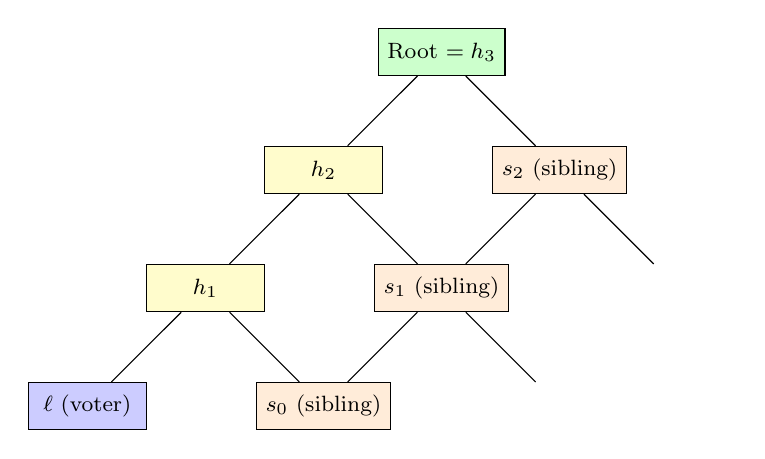
\begin{tikzpicture}[
    level distance=1.5cm,
    sibling distance=3cm,
    every node/.style={rectangle, draw, minimum width=1.5cm, minimum height=0.6cm, font=\footnotesize},
    edge from parent/.style={draw, -}
]
\node[fill=green!20] {Root $= h_3$}
    child {node[fill=yellow!20] {$h_2$}
        child {node[fill=yellow!20] {$h_1$}
            child {node[fill=blue!20] {$\ell$ (voter)}}
            child {node[fill=orange!15] {$s_0$ (sibling)}}
        }
        child {node[fill=orange!15] {$s_1$ (sibling)}
            child[draw=none] {node[draw=none] {}}
            child[draw=none] {node[draw=none] {}}
        }
    }
    child {node[fill=orange!15] {$s_2$ (sibling)}
        child[draw=none] {node[draw=none] {}}
        child[draw=none] {node[draw=none] {}}
    };
\end{tikzpicture}
\caption{Merkle proof structure: the voter (blue) provides siblings (orange) to reconstruct the root (green). Only the path from leaf to root is needed-the rest of the tree remains hidden.}
\label{fig:merkle_proof}
\end{figure}

\subsubsection{Lean Incremental Merkle Tree}

Traditional Merkle trees require pre-allocation of all leaves. The \textit{Lean Incremental Merkle Tree} (LeanIMT) optimizes storage by only maintaining the ``frontier''-the rightmost node at each level-and computing internal nodes on-demand. This reduces on-chain storage from $O(n)$ to $O(\log n)$.

\subsection{Non-Interactive Zero-Knowledge Proofs (NIZKs)}

While interactive ZK proofs \cite{goldwasser1985knowledge} require back-and-forth communication, blockchain applications require \textit{non-interactive} proofs-a single message from prover to verifier. The transformation from interactive to non-interactive was first achieved by Blum, Feldman, and Micali (1988) \cite{blum1988noninteractive} using a common reference string (CRS), and later by Fiat and Shamir \cite{fiat1986prove} using a random oracle (hash function) to simulate the verifier's challenges.

A NIZK proof system consists of three algorithms:

\begin{equation}
\pi \leftarrow \text{Prove}(pk, x, w) \quad ; \quad b \leftarrow \text{Verify}(vk, x, \pi)
\label{eq:nizk}
\end{equation}

Where:
\begin{itemize}
    \item $pk$ - proving key (public parameters for proof generation)
    \item $vk$ - verification key (public parameters for proof checking)
    \item $x$ - public inputs (statement to be verified)
    \item $w$ - witness (private inputs known only to the prover)
    \item $\pi$ - proof (succinct, constant-size)
    \item $b$ - boolean verdict (accept/reject)
\end{itemize}

\textbf{Succinctness} is a critical property: the proof size $|\pi|$ and verification time must be much smaller than the computation being proven. Formally, for a relation $\mathcal{R}$ with witness of size $n$, we require $|\pi| = O(\text{polylog}(n))$ and $T_{\text{verify}} = O(\text{polylog}(n))$. This property enables practical blockchain deployment-the on-chain verifier performs constant-time work regardless of the circuit complexity.

\subsubsection{Arithmetization: From Computation to Constraints}

Before a ZK proof can be generated, the computation must be expressed as an arithmetic circuit over a finite field-a process called \textit{arithmetization}. Modern proving systems use different arithmetization schemes:

\begin{itemize}
    \item \textbf{R1CS (Rank-1 Constraint System):} Used by Groth16 and Circom. Represents constraints as $\vec{a} \cdot \vec{s} \times \vec{b} \cdot \vec{s} = \vec{c} \cdot \vec{s}$ where $\vec{s}$ is the witness vector. Each constraint captures one multiplication gate.
    
    \item \textbf{PLONKish Arithmetization:} Used by PLONK \cite{gabizon2019plonk} and UltraHonk \cite{aztec2024ultrahonk}. Represents constraints as entries in a \textit{trace table} with custom gates. Each row encodes a gate: $q_L \cdot w_L + q_R \cdot w_R + q_O \cdot w_O + q_M \cdot w_L \cdot w_R + q_C = 0$, where $q_*$ are selector polynomials and $w_*$ are wire values. This is more flexible than R1CS because:
    \begin{itemize}
        \item Custom gates can encode complex operations (e.g., range checks, lookups) in fewer rows
        \item Lookup tables enable efficient implementation of non-arithmetic operations
        \item The universal reference string (URS) is circuit-independent
    \end{itemize}
\end{itemize}

Our system uses UltraHonk's PLONKish arithmetization via the Noir compiler \cite{noir2024docs}, which automatically translates high-level Noir code into an optimized constraint system. The compiled circuit contains 19,278 gates-substantially fewer than an equivalent Circom circuit due to UltraHonk's custom gates for Poseidon and range checks.

\subsubsection{ZK-SNARKs vs.\ ZK-STARKs}

The two dominant families of succinct zero-knowledge proof systems differ fundamentally in their cryptographic assumptions and performance characteristics:

\textbf{ZK-SNARKs} (Zero-Knowledge Succinct Non-interactive Arguments of Knowledge) \cite{groth2016size} rely on bilinear pairings over elliptic curves (e.g., BN254, BLS12-381). They achieve the smallest proof sizes (128 bytes for Groth16) but historically required a \textit{trusted setup}-a ceremony that generates structured reference strings (SRS). If the ceremony is compromised, an adversary can forge proofs that pass verification, completely undermining the system. Recent pairing-based systems (PLONK, UltraHonk) eliminate per-circuit trusted setups by using a universal or transparent reference string \cite{gabizon2019plonk}.

\textbf{ZK-STARKs} (Zero-Knowledge Scalable Transparent Arguments of Knowledge) rely only on hash functions, making them \textit{transparent} (no trusted setup) and potentially post-quantum secure. However, they produce significantly larger proofs ($\sim$100 KB vs. $\sim$128 bytes for Groth16) and have slower verification.

\textbf{UltraHonk} (our choice) represents a middle ground: it is a pairing-based system that achieves \textit{no trusted setup} through a transparent commitment scheme (IPA or KZG with powers-of-tau), produces moderately-sized proofs ($\sim$14 KB), and provides fast verification suitable for on-chain deployment. The key insight is that UltraHonk's transparent setup means no party must be trusted during system initialization-a critical property for election integrity \\cite{aztec2024ultrahonk}.

\begin{table}[H]
\centering
\caption{Comparison of ZK proof systems}
\label{tab:zk_systems}
\begin{tabular}{|l|c|c|c|c|}
\hline
\textbf{Property} & \textbf{Groth16} & \textbf{PLONK} & \textbf{UltraHonk} & \textbf{STARKs} \\ \hline
Trusted setup & Per-circuit & Universal & \textbf{None} & None \\ \hline
Proof size & 128 bytes & 400 bytes & \textbf{$\sim$14 KB} & $\sim$100 KB \\ \hline
Verification time & Fast & Fast & \textbf{Fast} & Slower \\ \hline
Prover time & Moderate & Moderate & \textbf{Fast} & Fast \\ \hline
Post-quantum secure & No & No & No & Yes \\ \hline
\end{tabular}
\end{table}

Our system uses \textbf{UltraHonk} (from Aztec's Barretenberg library) which requires \textbf{no trusted setup}-eliminating a significant security concern where a compromised setup ceremony could allow forged proofs. The Zerocash protocol \cite{sasson2014zerocash}, which pioneered the use of ZK-SNARKs for anonymous transactions, demonstrated both the power and the practical difficulty of trusted setup ceremonies. Similar privacy-preserving constructions have been applied in systems like Hawk \cite{kosba2016hawk} and Zcash \cite{zcash2016protocol}. The Semaphore protocol \cite{semaphore2020} provides a closely related ZK-based anonymous signaling primitive on Ethereum. Our adoption of UltraHonk avoids the trusted setup challenge entirely while maintaining efficient on-chain verification.

\subsection{Privacy Models in E-Voting}

Understanding the different privacy models is essential for evaluating e-voting systems. We distinguish three levels of privacy guarantees:

\begin{enumerate}
    \item \textbf{Computational Privacy (Encryption-based):} Privacy holds as long as the adversary cannot break the underlying encryption scheme. A sufficiently powerful adversary (e.g., one with access to decryption keys or quantum computers) can violate privacy. Examples: Estonia (RSA encryption), homomorphic tallying systems.
    
    \item \textbf{Information-Theoretic Privacy (Secret Sharing):} Privacy holds unconditionally, regardless of computational power, provided a threshold of servers remains honest. Example: Threshold decryption schemes where $k$-of-$n$ servers must collude.
    
    \item \textbf{Zero-Knowledge Privacy (Our Approach):} The proof reveals \textit{mathematically nothing} beyond the truth of the statement. No decryption key exists. Even a computationally unbounded adversary learns nothing about the voter's identity from the proof. The privacy guarantee relies on the zero-knowledge property of the proof system (which is information-theoretic in the random oracle model).
\end{enumerate}

This distinction is critical: in encryption-based systems (models 1 and 2), some party or threshold of parties \textit{could} in principle decrypt votes. In our ZK-based system, no such capability exists-the voter's identity is never encrypted; it is simply never revealed.

\newpage
\section{Previous Work}

Electronic voting systems built on blockchain have been extensively studied due to the limitations of traditional systems in security, transparency, verifiability, and decentralization. The immutable ledger and decentralized consensus mechanisms provided by blockchain enable tamper-resistant vote recording and unbiased verification of election outcomes \cite{mdpi2024evoting, hajian2024blockchain, cluster2024blockchain}. Various blockchain architectures have been proposed-permissioned, permissionless, and hybrid-each with trade-offs in security, transparency, and performance \cite{kho2022review}.

Research has examined scalable blockchain-based voting models that balance security, decentralization, and performance for large-scale elections \cite{mdpi2022scalability, abuidris2021secure}. Most employ sharding and hybrid consensus mechanisms to enhance transaction throughput while maintaining system integrity.

Emerging research also addresses post-quantum security concerns, proposing quantum-resistant cryptographic techniques for blockchain-enabled e-voting systems \cite{arxiv2024quantum, mandal2024hybrid, alshahrani2021endtoend}.

\subsection{Centralized E-Voting Systems}

\subsubsection{Estonia's Internet Voting System}
The world's first e-voting system was implemented in Estonia in 2005 and remains operational \cite{madise2005evoting}. Authentication uses a national ID card with PIN. Votes are transmitted from the Vote Forwarding Server (VFS) to the Vote Storage Server (VSS), where encrypted votes are stored until the election period ends. Transaction logs are recorded in the Log Server \cite{ivoting-ccs2014}. After voting closes, votes in VSS are stripped of identifying information and transferred to the air-gapped Vote Counting Server (VCS) via DVD for decryption and tallying \cite{ivxv_protocols2022}.

\begin{figure}[H]
    \centering
    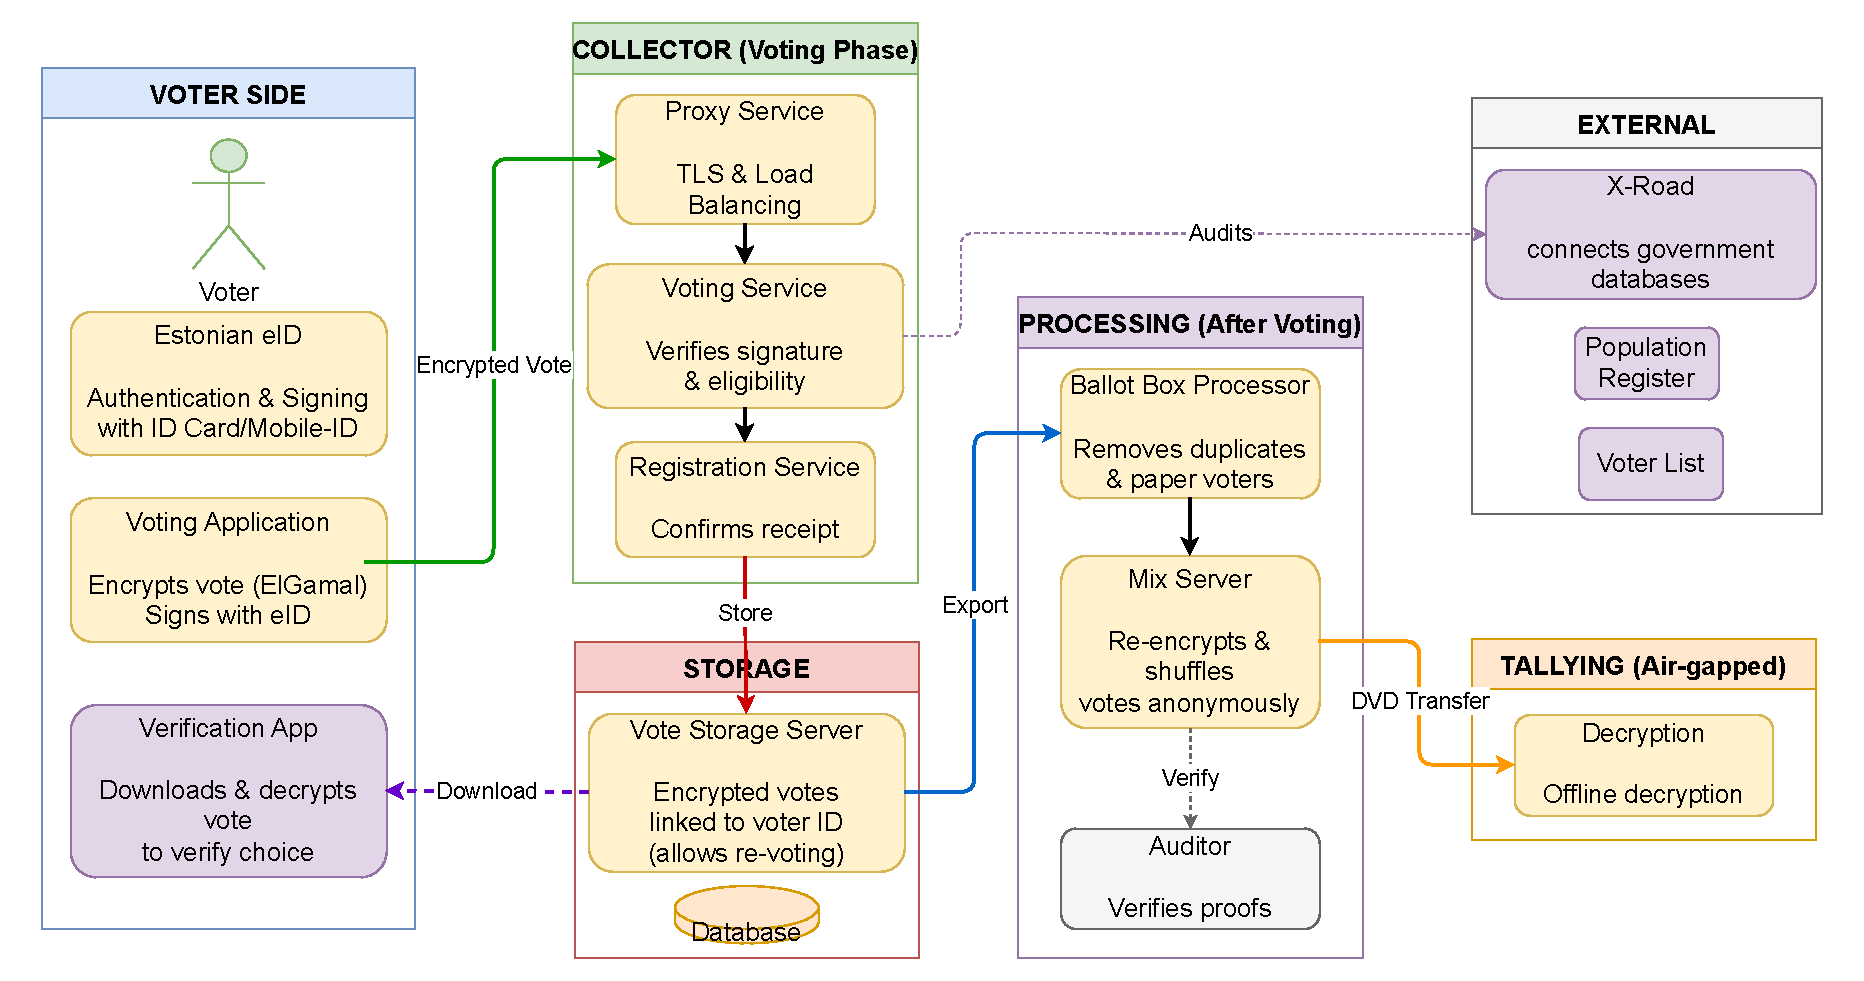
\includegraphics[width=1\textwidth]{estonia_architecture.pdf}
    \caption{High-level architecture of Estonia's e-voting system}
    \label{fig:estonia_architecture}
\end{figure}

The system allows re-voting (only the last vote counts) to mitigate coercion \cite{ivoting-ccs2014, sutopo2024identifying}. Key limitations include:
\begin{enumerate}
  \item Centralized architecture creating a single point of failure
  \item Insufficient transparency and over-reliance on institutional trust
  \item No mathematical privacy guarantee-administrators with access to decryption keys can theoretically link votes to voters
\end{enumerate}

\subsubsection{Australia's iVote System}
The iVote system, used in the 2015 NSW state election in Australia, represents the world's largest deployment of online voting with 280,000 ballots issued \cite{halderman2015ivote}.

\begin{figure}[H]
    \centering
    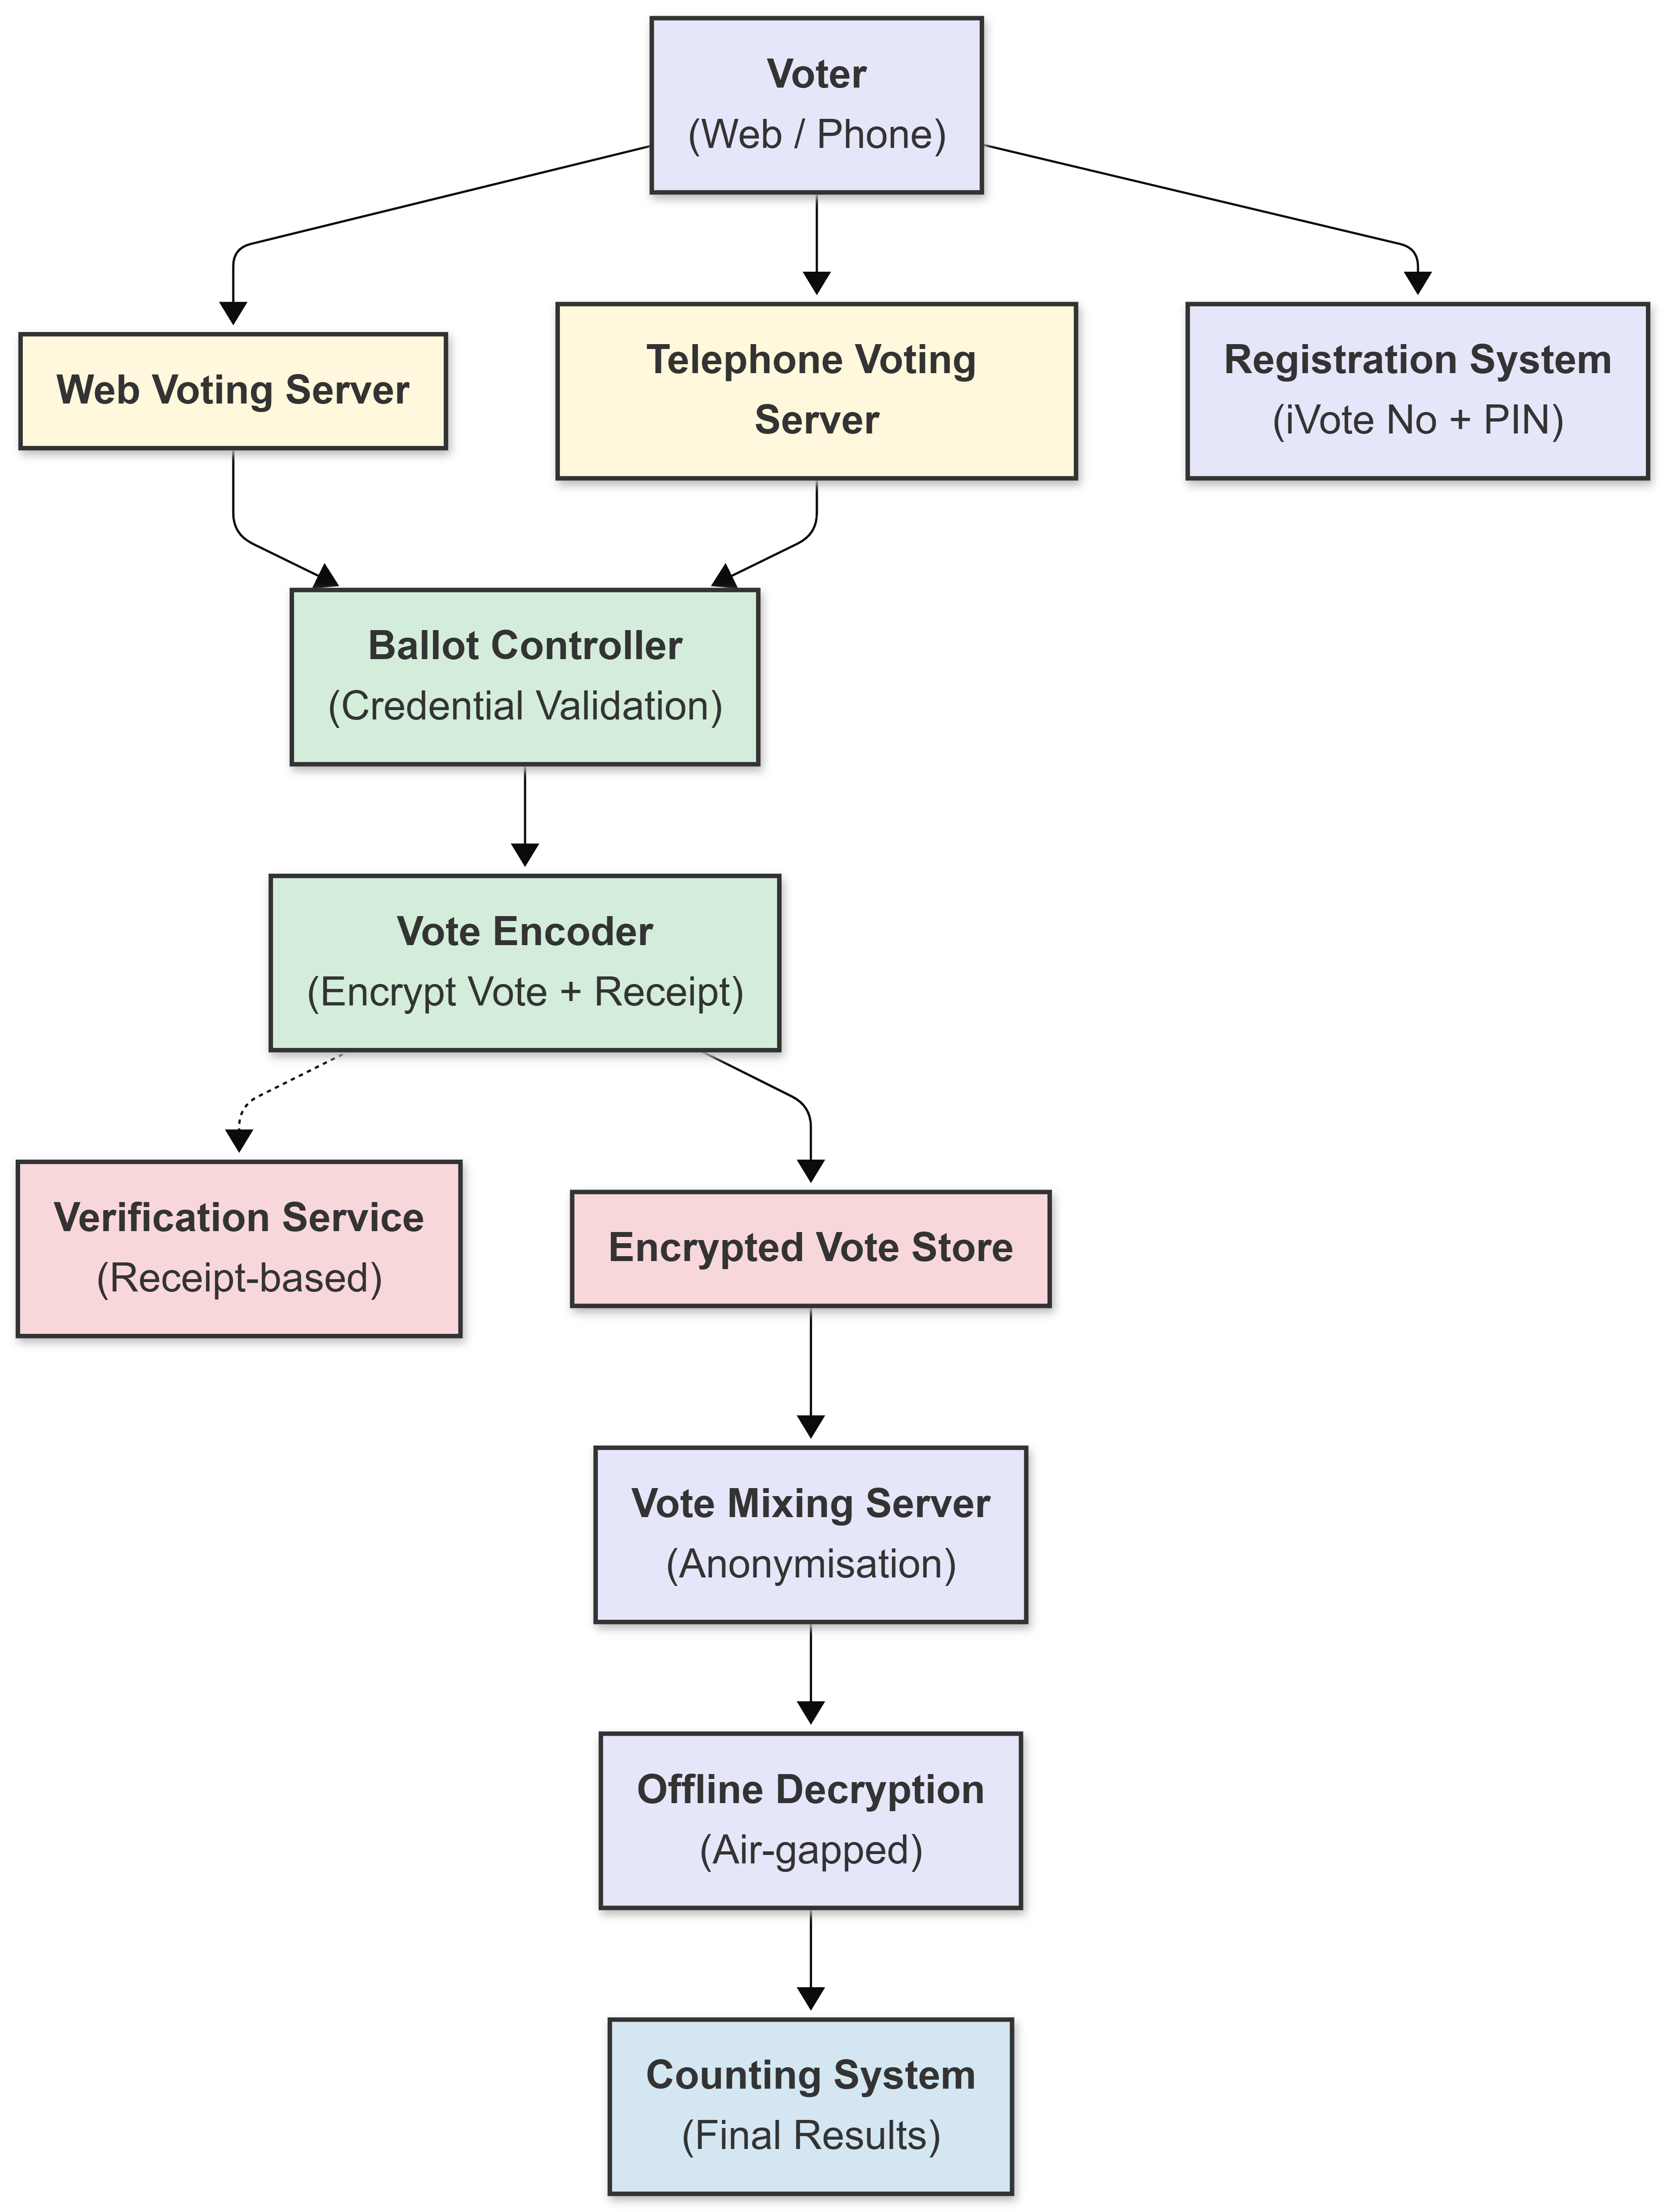
\includegraphics[width=0.9\textwidth]{ivote_architecture.png}
    \caption{High-level architecture of Australia's iVote system (2015 NSW State Election)}
    \label{fig:ivote-architecture}
\end{figure}

Security analysis during the election identified critical vulnerabilities. The use of insecure third-party JavaScript from \texttt{ivote.piwikpro.com} made the system susceptible to FREAK and Logjam attacks, enabling malicious code injection capable of altering vote content \cite{halderman2015ivote, nswec_2015_ivote_security}. Identified vulnerabilities include:
\begin{enumerate}
    \item Insecure external dependency loading (third-party JavaScript)
    \item Weak verification mechanism (4-digit receipt code)
    \item Lack of transparency and independent auditing capability
\end{enumerate}

\newpage
\subsection{Blockchain-Based E-Voting Systems}

\subsubsection{Sierra Leone's Blockchain Voting (2018)}
The first national election utilizing blockchain took place during Sierra Leone's 2018 presidential election \cite{acm2024_blockchain_voting_analysis}. Voters cast paper ballots; final counts from polling stations were later entered into a blockchain to create an immutable record \cite{chohan2018sierra_leone}. Limitations:
\begin{enumerate}
    \item Manual vote recording introduces human error and trust assumptions
    \item Permissioned server for vote verification maintains centralized control
    \item Blockchain used only for auditing, not for vote casting itself
\end{enumerate}

\subsubsection{Switzerland's Verifiable E-Voting Pilots (2023)}
Switzerland implemented the most architecturally advanced online voting system using client-side encryption, 4 Control Components for Mixing (CCMs) and 4 Control Components for Return Codes (CCRs) \cite{swisspost_gitlab_evoting}. Three CCMs are operated online by Swiss Post; one CCM is offline, operated by the Canton \cite{federalchancellery_evoting}.

\begin{figure}[H]
    \centering
    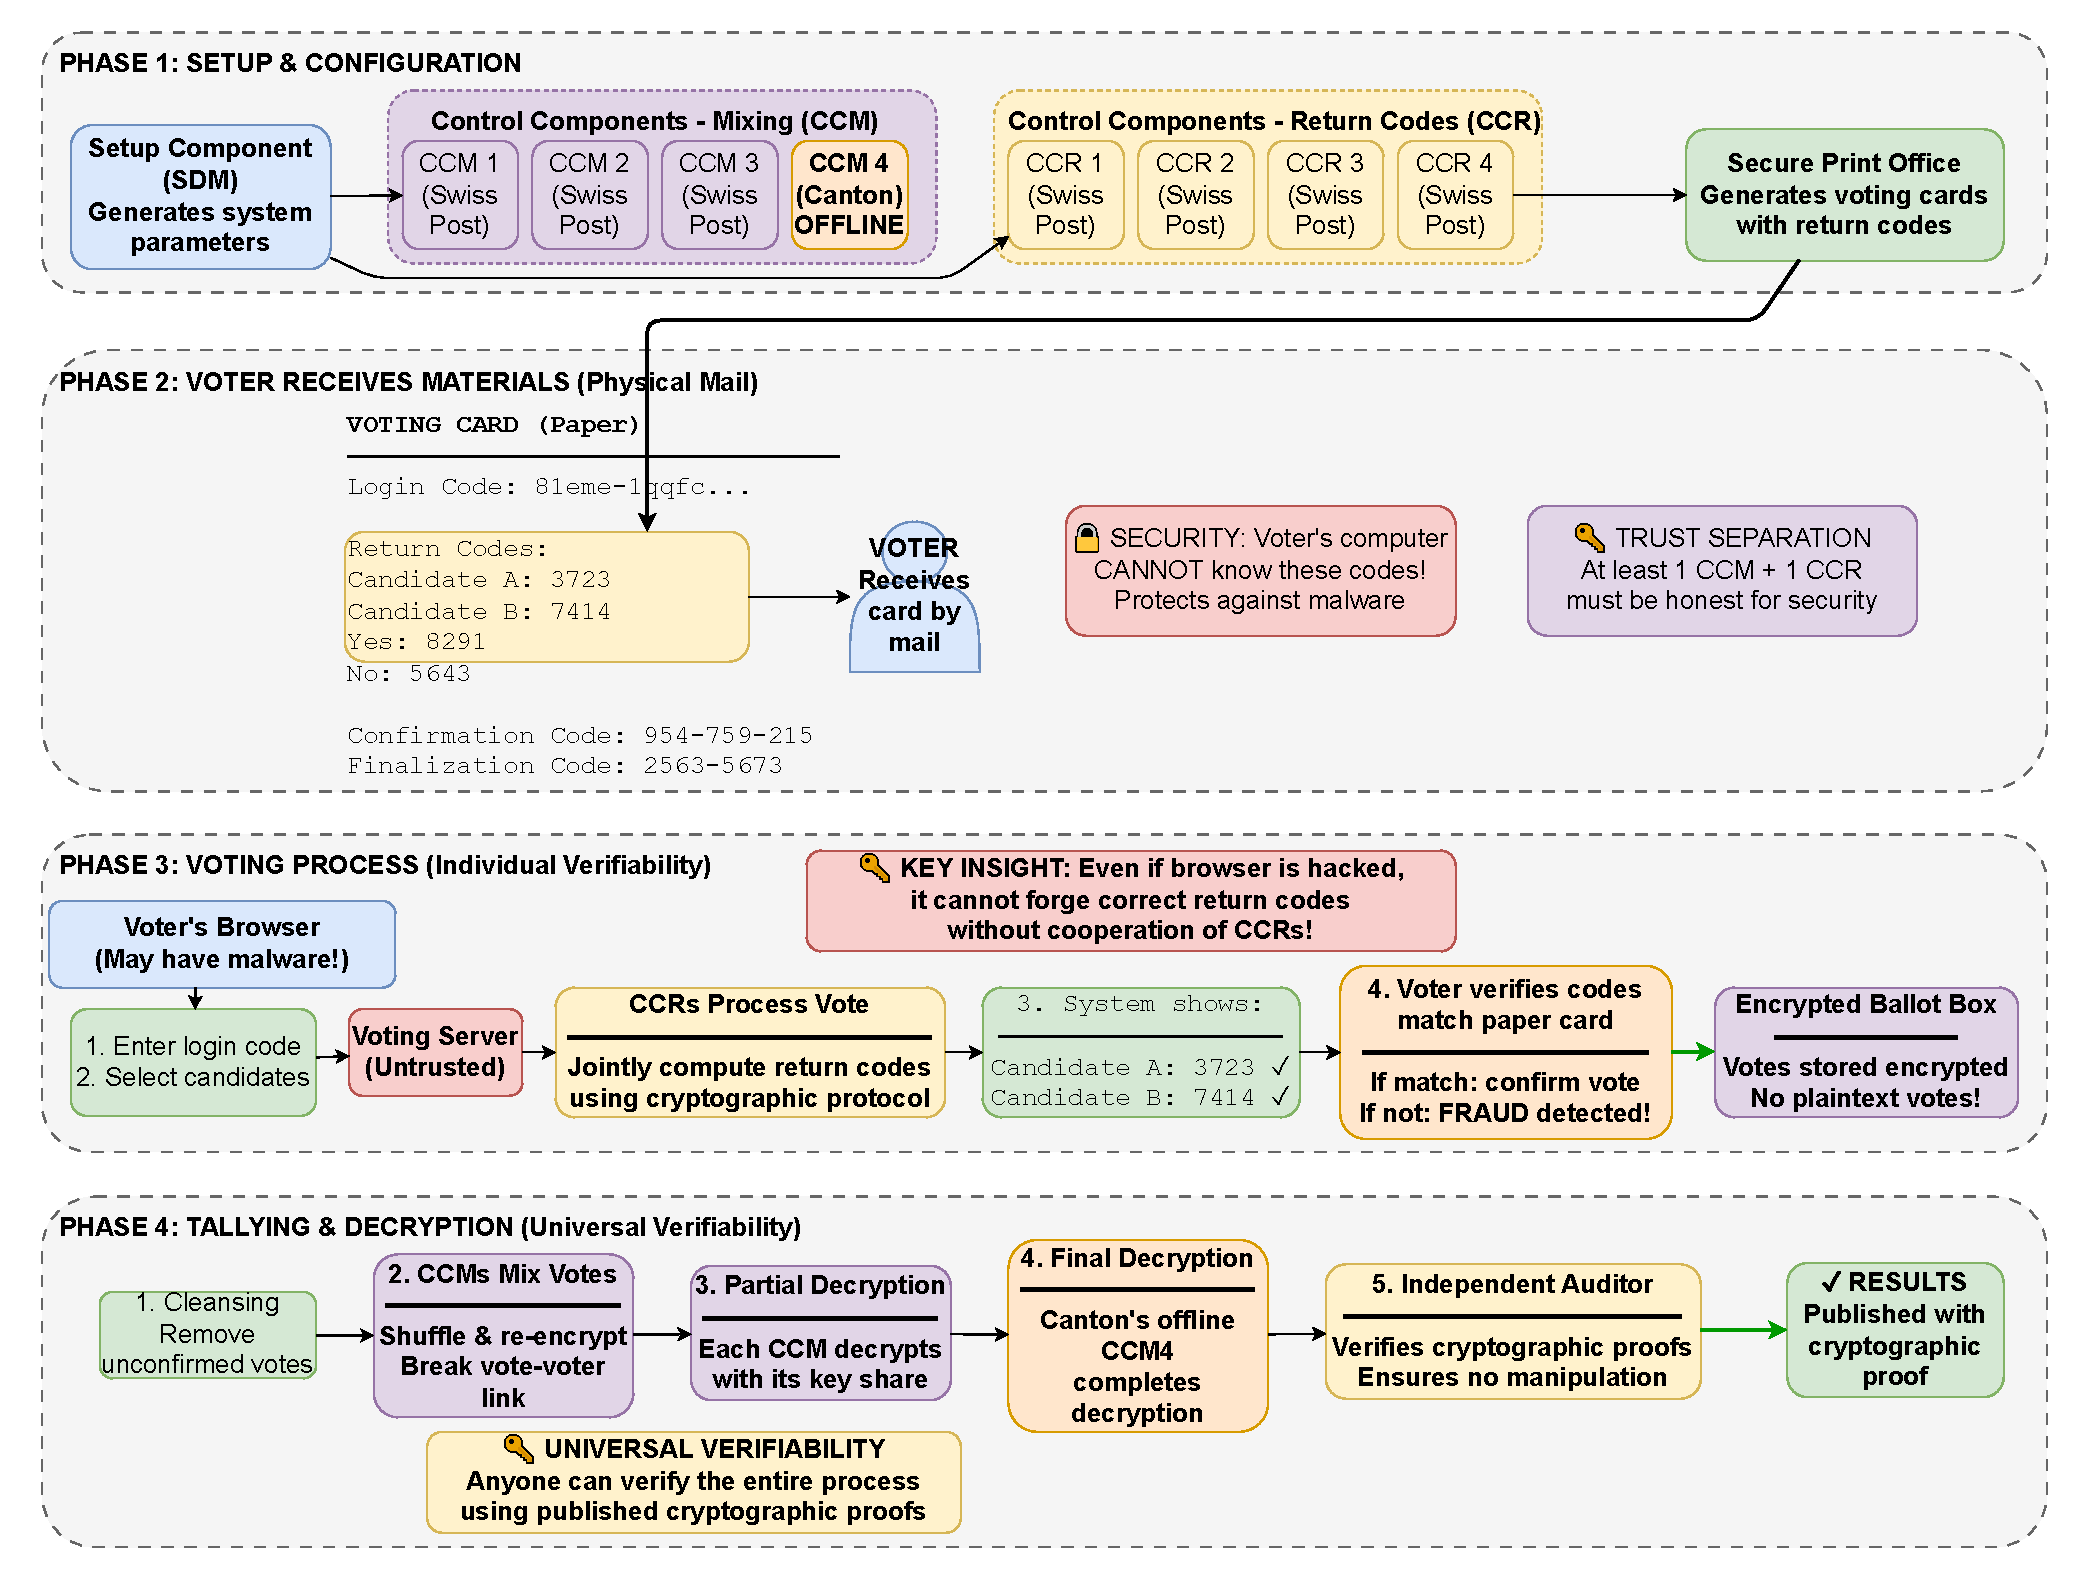
\includegraphics[width=1.1\textwidth,height=0.55\textheight]{swiss_evoting_pilot.pdf}
    \caption{Swiss Post Verifiable E-Voting System Architecture}
    \label{fig:swiss_evoting_pilot}
\end{figure}

This system achieves both individual verifiability (voters verify via paper return codes) and universal verifiability (cryptographic audit proofs published) \cite{ford2022_audit_swisspost}. However, it requires significant infrastructure and operational cost, and privacy still depends on the threshold assumption (at least one control component must be honest).

\subsection{Advanced Blockchain E-Voting Proposals}

\subsubsection{Quantum-Secure Mobile Voting System}
A team from BITS Pilani proposed a system using mobile biometric authentication with EtherJS smart contracts, achieving verifiability, fault tolerance, and quantum resilience \cite{poudel2025quantum_blockchain_evoting}. Limitations include accessibility issues from anti-spoofing biometric authentication and high Ethereum gas costs.

\subsubsection{FASTEN Protocol}
The FASTEN system uses Ethereum smart contracts for fair, secure, anonymous elections at approximately \$0.04 per vote-significantly cheaper than traditional elections (\$5.54 per vote)-but throughput is limited to approximately 20,000 votes per hour \cite{damle2021fasten}.

\subsection{Comparative Analysis}

Table~\ref{tab:comparison} compares existing systems and our implemented system across key evaluation criteria.

\begin{landscape}
\begin{table}[p]
\centering
\caption{Comparison of Existing E-Voting Systems with Our Implemented System}
\label{tab:comparison}
\begin{adjustbox}{max width=\linewidth}
\begin{tabular}{|c|m{3.5cm}|c|c|c|c|c|m{4.5cm}|}
\hline
\textbf{Ref.} & \textbf{System} & \textbf{Privacy} & \textbf{E2E Verifiable} & \textbf{Decentralized} & \textbf{Scalable} & \textbf{Cost Efficient} & \textbf{Key Limitations} \\ \hline

\cite{madise2005evoting} & Estonian Internet Voting & Partial & No & No & Yes & Yes & Centralized, no E2E verifiability \\ \hline

\cite{halderman2015ivote} & iVote (Australia) & Partial & Weak & No & Yes & Yes & Client-side attacks, third-party scripts \\ \hline

\cite{chohan2018sierra_leone} & Sierra Leone Blockchain & No & No & Partial & Yes & Yes & Manual entry, centralized verification \\ \hline

\cite{federalchancellery_evoting} & Swiss Post E-Voting & Yes & Yes & Partial & Yes & No & High cost, complex infrastructure \\ \hline

\cite{abuidris2021secure} & Hybrid Consensus & Yes & Partial & Yes & Partial & No & High complexity, performance overhead \\ \hline

\cite{damle2021fasten} & FASTEN Protocol & Yes & Yes & Yes & No & Yes & Limited throughput (\textasciitilde20k/hour) \\ \hline

\cite{poudel2025quantum_blockchain_evoting} & Quantum-Secure Mobile & Yes & Yes & Yes & Partial & No & High gas costs, accessibility issues \\ \hline

-- & \textbf{Our System} & \textbf{Yes} & \textbf{Yes} & \textbf{Yes} & \textbf{Prototype} & \textbf{Optimized} & \textbf{Local testnet deployment} \\ \hline

\end{tabular}
\end{adjustbox}
\end{table}
\end{landscape}

Our system achieves full privacy through ZK proofs (no trusted decryptor needed), end-to-end verifiability through on-chain proof verification, and decentralization through smart contract-based logic with no central authority controlling the tally. The primary limitation is that the current implementation operates on a local testnet rather than a production blockchain.

\newpage
\section{Gaps in Literature}
\begin{enumerate}
    \item \textbf{Client-Side Proof Generation:} Most proposed ZK-voting systems assume server-side proof generation or specialized hardware, but few demonstrate complete browser-based proof generation accessible to ordinary users \cite{mdpi2024evoting, vladucu2023evoting}.
    
    \item \textbf{Practical Implementation:} Many papers propose theoretical architectures without providing functional prototypes or demonstrating end-to-end workflows from registration through anonymous vote casting \cite{mdpi2022scalability, prajapat2020investigating}.
    
    \item \textbf{Purpose-Built Blockchain:} Most systems deploy on Ethereum or Hyperledger, inheriting their complexity (gas fees, wallet management, EVM overhead). No existing work combines a custom election-specific blockchain with ZK proofs.
    
    \item \textbf{Trusted Setup Elimination:} Systems using Groth16 (Circom/snarkjs) require trusted setup ceremonies that are difficult to verify and represent an attack vector.
    
    \item \textbf{Usability:} Insufficient attention is given to user experience-voters should not need to understand cryptography or manage cryptocurrency wallets \cite{mdpi2024evoting, vladucu2023evoting}.
\end{enumerate}

Our implementation addresses all five gaps by providing: a functional prototype with browser-based proof generation (Gap 1\&2), a custom Go blockchain (Gap 3), UltraHonk proving with no trusted setup (Gap 4), and an intuitive web interface requiring no wallet extensions (Gap 5).


%%%%%%%%%%%%%%%%%%%%%%%%%%%%%%%%%%%%%
% CHAPTER 3: METHODOLOGY
%%%%%%%%%%%%%%%%%%%%%%%%%%%%%%%%%%%%%
\chapter{Methodology}

\section{Overview of System Architecture}

The system follows a dual-track development methodology:

\begin{enumerate}
    \item \textbf{Track A - ZK Voting Application (this report's primary focus):} The complete voting workflow including ZK circuit design, smart contract logic, frontend proof generation, and anonymous vote casting. Currently operational on a local Ethereum-compatible blockchain (Hardhat) for rapid iteration and testing.
    
    \item \textbf{Track B - Custom Blockchain (parallel development):} A purpose-built blockchain in Go, optimized for election administration. Designed to replace the Ethereum layer once the voting logic is proven correct, eliminating gas fees, wallet requirements, and EVM overhead.
\end{enumerate}

Both tracks share the same cryptographic primitives (Poseidon hash, Noir ZK circuit, UltraHonk proofs), ensuring seamless migration when Track B reaches maturity.

\begin{figure}[H]
    \centering
    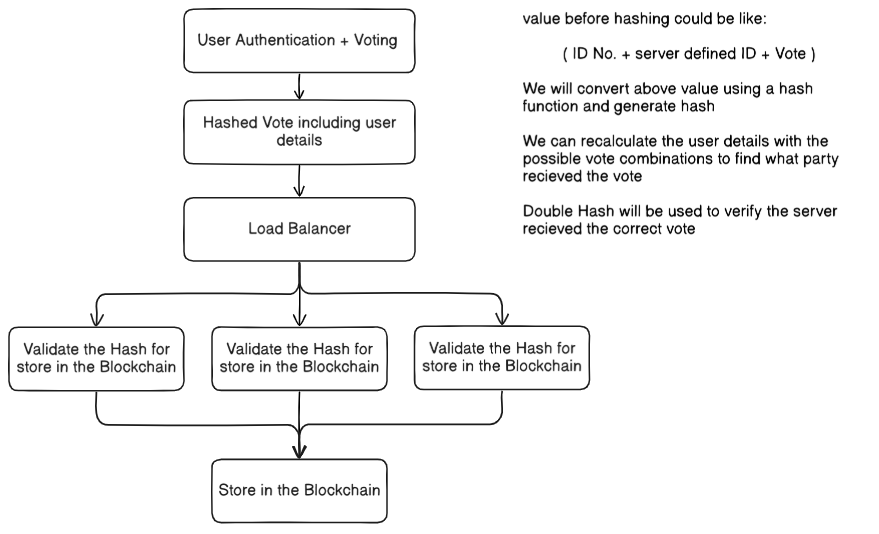
\includegraphics[width=\textwidth]{Top_Level_Architecture.png}
    \caption{High-level system architecture showing the interaction between the ZK application layer, the blockchain layer, and the cryptographic proof system}
    \label{fig:top_level_arch}
\end{figure}

\subsection{Development Methodology}

The system was developed using an iterative methodology, progressing through clearly defined implementation phases. Each phase built upon the previous one, with verification at each stage before proceeding. This approach allowed early identification and resolution of issues, ensuring a stable foundation for subsequent development.

\begin{figure}[H]
    \centering
    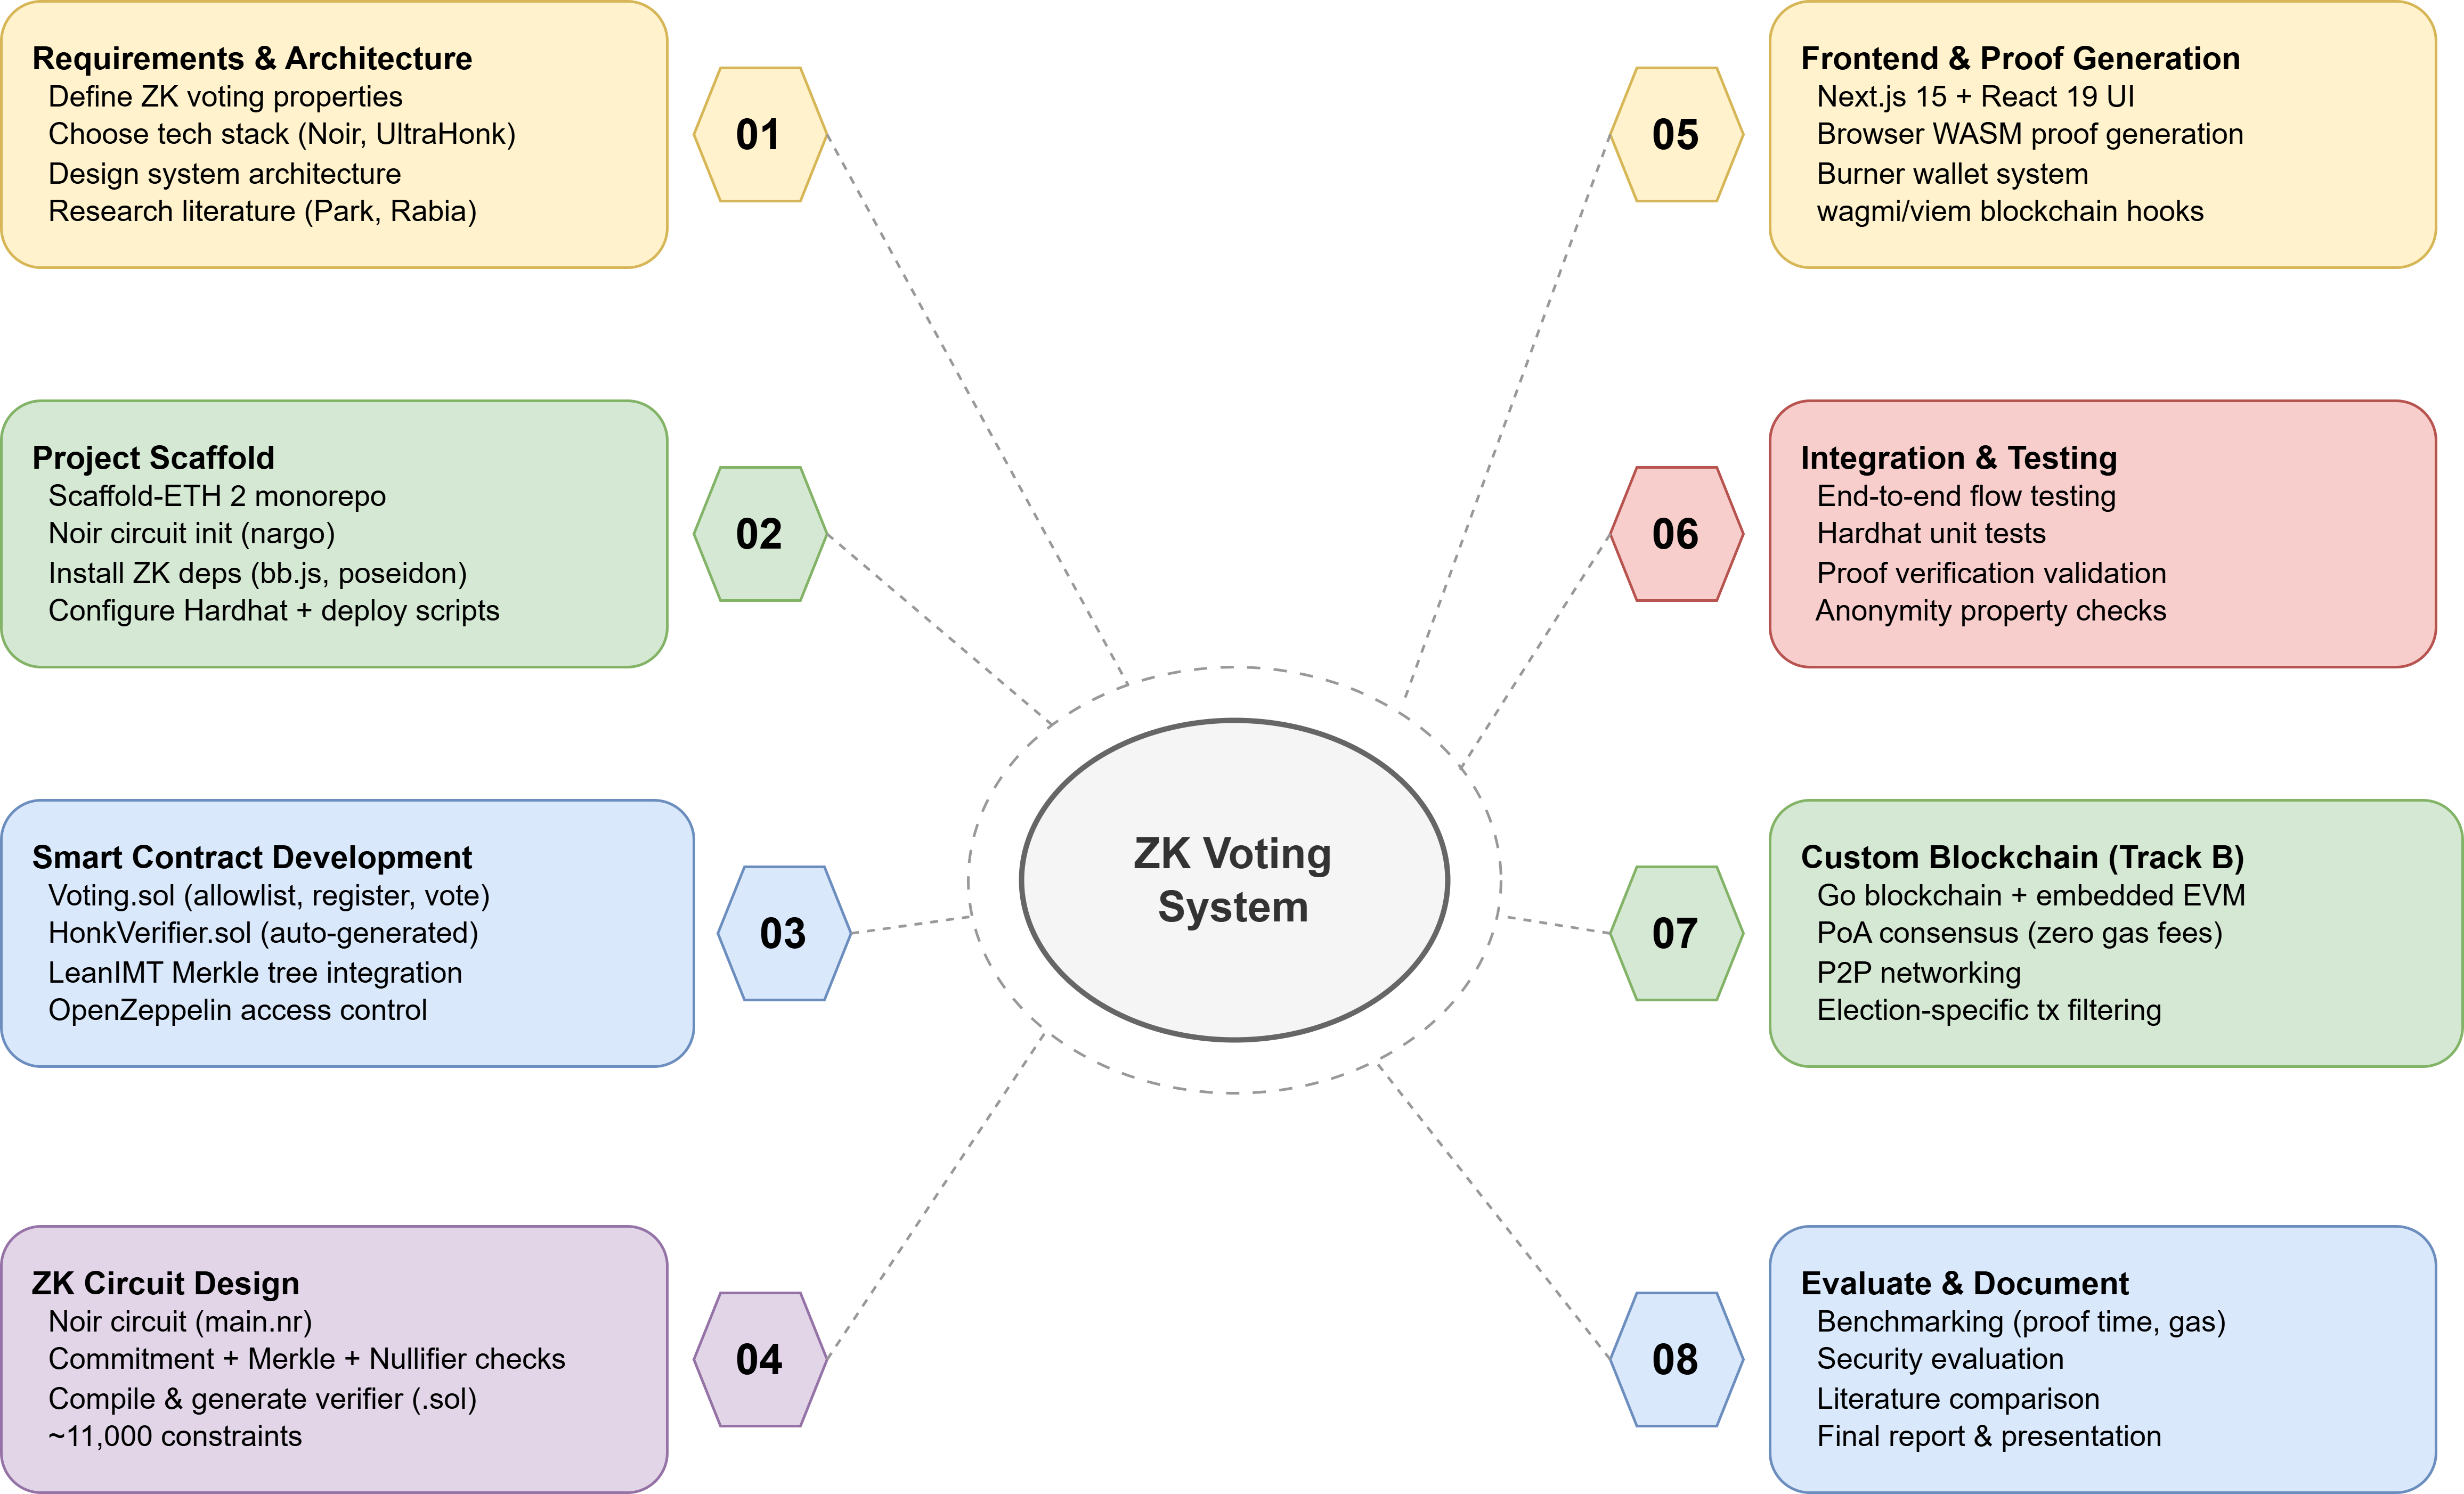
\includegraphics[width=\textwidth]{workflow.png}
    \caption{Development workflow overview showing the iterative methodology}
    \label{fig:workflow}
\end{figure}

\newpage
\section{Cryptographic Design}

This section formally defines the cryptographic building blocks of the system.

\subsection{Commitment Scheme}

A \textit{commitment scheme} allows a party to commit to a value while keeping it hidden, with the ability to reveal it later. Our scheme uses Poseidon hashing:

\begin{equation}
\boxed{C = \text{Poseidon}_2(\text{nullifier}, \text{secret})}
\label{eq:commitment}
\end{equation}

Where:
\begin{itemize}
    \item $\text{nullifier} \xleftarrow{\$} \mathbb{F}_p$ - a cryptographically random field element (256 bits of entropy)
    \item $\text{secret} \xleftarrow{\$} \mathbb{F}_p$ - an independent random field element
    \item $C \in \mathbb{F}_p$ - the commitment (publicly stored on-chain)
\end{itemize}

\textbf{Security Properties:}
\begin{itemize}
    \item \textbf{Binding:} Given $C$, it is computationally infeasible to find $(n', s') \neq (n, s)$ such that $\text{Poseidon}_2(n', s') = C$ (collision resistance of Poseidon)
    \item \textbf{Hiding:} Given $C$, it reveals no information about $n$ or $s$ (preimage resistance of Poseidon)
\end{itemize}

\textbf{Numerical Example:}

Let us trace through with concrete (simplified) values to illustrate the scheme:
\begin{align}
\text{nullifier} &= 0x1a2b3c\ldots \quad \text{(random 254-bit field element)} \\
\text{secret} &= 0x4d5e6f\ldots \quad \text{(independent random element)} \\
C &= \text{Poseidon}_2(0x1a2b3c\ldots, 0x4d5e6f\ldots) = 0x7f8a9b\ldots
\end{align}

The commitment $C$ is stored on-chain. The voter retains $(n, s)$ privately in their browser's localStorage.

\subsection{Nullifier Scheme}

To prevent double-voting without revealing which commitment is voting:

\begin{equation}
\boxed{N_h = \text{Poseidon}_1(\text{nullifier})}
\label{eq:nullifier}
\end{equation}

\textbf{Why this works:}
\begin{itemize}
    \item Each voter has exactly one nullifier (generated during registration)
    \item Each nullifier produces exactly one nullifier hash $N_h$ (deterministic)
    \item When voting, $N_h$ is revealed publicly and stored on-chain
    \item If the same voter tries to vote again, the contract detects the duplicate $N_h$
    \item Given only $N_h$, finding the original nullifier requires breaking Poseidon's preimage resistance
    \item The commitment $C = \text{Poseidon}_2(n, s)$ and the nullifier hash $N_h = \text{Poseidon}_1(n)$ are \textit{unlinkable} without knowledge of $n$
\end{itemize}

\begin{figure}[H]
\centering
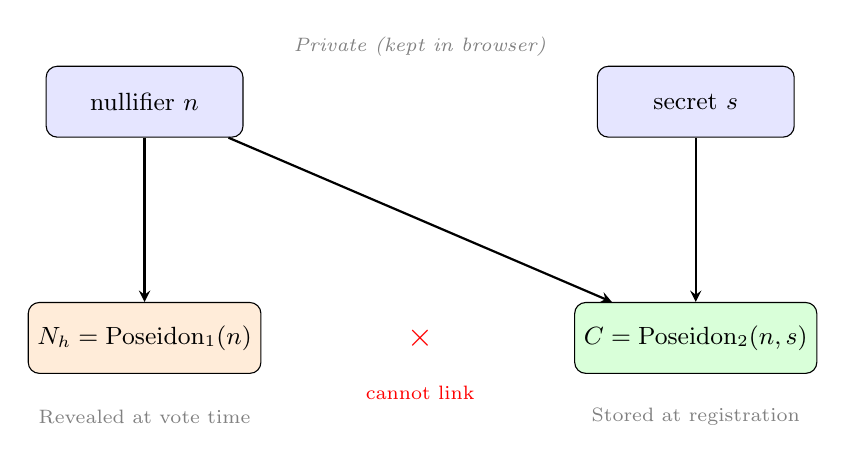
\begin{tikzpicture}[
    box/.style={rectangle, draw, rounded corners, minimum width=2.5cm, minimum height=0.9cm, font=\small, align=center},
    arrow/.style={->, thick, >=stealth}
]
    % Private inputs at top, widely spaced
    \node[box, fill=blue!10] (null) at (0,0) {nullifier $n$};
    \node[box, fill=blue!10] (sec) at (7,0) {secret $s$};
    
    % Label
    \node[font=\scriptsize, text=gray] at (3.5,0.7) {\textit{Private (kept in browser)}};
    
    % Outputs well below, widely spaced
    \node[box, fill=orange!15] (nhash) at (0,-3) {$N_h = \text{Poseidon}_1(n)$};
    \node[box, fill=green!15] (commit) at (7,-3) {$C = \text{Poseidon}_2(n, s)$};
    
    % Simple straight arrows down
    \draw[arrow] (null) -- (nhash);
    \draw[arrow] (null) -- (commit);
    \draw[arrow] (sec) -- (commit);
    
    % Red X between the two outputs
    \node[font=\large, text=red] at (3.5,-3) {\textbf{$\times$}};
    \node[font=\scriptsize, text=red] at (3.5,-3.7) {cannot link};
    
    % Labels below outputs
    \node[font=\scriptsize, text=gray] at (0,-4) {Revealed at vote time};
    \node[font=\scriptsize, text=gray] at (7,-4) {Stored at registration};
\end{tikzpicture}
\caption{Nullifier scheme: the voter's private nullifier $n$ produces two public values-$N_h$ (for double-vote prevention) and $C$ (for membership registration). Without knowing $n$, an observer cannot link them.}
\label{fig:nullifier_scheme}
\end{figure}

\subsection{Merkle Tree Membership Proof}

All voter commitments are stored in a Lean Incremental Merkle Tree using Poseidon as the internal hash:

\begin{equation}
\text{parent} = \text{Poseidon}_2(\text{left\_child}, \text{right\_child})
\label{eq:merkle_parent}
\end{equation}

The tree supports up to $2^{16} = 65{,}536$ leaves (voters). To prove membership, the voter provides:
\begin{itemize}
    \item Their commitment (recomputed from nullifier + secret inside the circuit)
    \item Their leaf index $j$ (private-keeps the voter's position hidden)
    \item The sibling hashes $[s_0, s_1, \ldots, s_{15}]$ along the path from leaf to root (private)
\end{itemize}

The circuit recomputes the root using Equation~\ref{eq:merkle_verify} and asserts it matches the public on-chain root.

\subsection{Combined ZK Statement}

The complete statement proven by our ZK circuit can be expressed as:

\begin{equation}
\boxed{
\begin{aligned}
&\text{Given public inputs } (N_h, R, v, d): \\
&\exists \, (n, s, j, \vec{S}) \text{ such that:} \\
&\quad (1) \; N_h = \text{Poseidon}_1(n) \\
&\quad (2) \; C = \text{Poseidon}_2(n, s) \\
&\quad (3) \; \text{MerkleVerify}(C, j, \vec{S}, d) = R \\
&\quad (4) \; v \in \{0, 1\}
\end{aligned}
}
\label{eq:zk_statement}
\end{equation}

Where:
\begin{itemize}
    \item $N_h$ - nullifier hash (public, prevents double-voting)
    \item $R$ - Merkle root (public, ensures proof is for the current tree state)
    \item $v$ - vote choice (public, bound to the proof so it cannot be changed)
    \item $d$ - tree depth (public)
    \item $n$ - nullifier (private)
    \item $s$ - secret (private)
    \item $j$ - leaf index (private, protects voter position)
    \item $\vec{S}$ - sibling array (private, Merkle authentication path)
\end{itemize}

\subsection{Security Properties}

\begin{table}[H]
\centering
\caption{Security properties achieved by the cryptographic design}
\label{tab:security_properties}
\begin{tabular}{|l|p{9cm}|}
\hline
\textbf{Property} & \textbf{How It Is Achieved} \\ \hline
Voter Anonymity & ZK proof reveals nothing about which leaf (voter) is proving membership; identity separation breaks address linkage \\ \hline
Double-Vote Prevention & Nullifier hash is deterministic per voter-submitting twice produces the same $N_h$, which the contract rejects \\ \hline
Vote Integrity & Vote choice is a public input bound to the ZK proof; changing the vote invalidates the proof \\ \hline
Eligibility & Only commitments in the Merkle tree can produce valid proofs; tree insertion is restricted to authorized voters \\ \hline
Non-Repudiation & Once a valid proof is accepted on-chain, the vote is permanently recorded in the immutable ledger \\ \hline
Coercion Resistance & Voter cannot prove to a coercer how they voted (proof is consumed by anonymous submission; no receipt links identity to vote) \\ \hline
\end{tabular}
\end{table}

\subsection{Formal Threat Model}

We define the adversary model and security assumptions under which our system provides its guarantees.

\subsubsection{Adversary Capabilities}

We consider a computationally bounded adversary $\mathcal{A}$ (probabilistic polynomial-time) with the following capabilities:

\begin{enumerate}
    \item \textbf{Network observation:} $\mathcal{A}$ can observe all on-chain transactions, including proof data, nullifier hashes, vote values, and transaction metadata (sender address, timestamp, gas price).
    
    \item \textbf{Partial system control:} $\mathcal{A}$ may control some voter accounts (Sybil attack) but cannot control the contract owner account or the blockchain consensus mechanism.
    
    \item \textbf{Proof manipulation:} $\mathcal{A}$ may attempt to forge proofs, replay valid proofs with altered public inputs, or extract private witness data from observed proofs.
    
    \item \textbf{Smart contract interaction:} $\mathcal{A}$ can call any public function on the deployed contracts and analyze the contract bytecode.
\end{enumerate}

\subsubsection{Security Assumptions}

\begin{enumerate}
    \item \textbf{Poseidon hash security:} The Poseidon hash function over BN254 provides at least 128 bits of security against preimage, second preimage, and collision attacks \cite{grassi2021poseidon}.
    
    \item \textbf{Discrete logarithm hardness:} The elliptic curve discrete logarithm problem on BN254 is computationally intractable for PPT adversaries. This underpins the soundness of the UltraHonk proof system.
    
    \item \textbf{Random oracle model:} The Fiat-Shamir heuristic (used to make proofs non-interactive) is modeled as a random oracle. The zero-knowledge property holds information-theoretically in this model.
    
    \item \textbf{Client-side integrity:} The voter's browser and local environment are not compromised by malware during proof generation. This is a standard assumption shared by all client-side cryptographic systems.
    
    \item \textbf{Blockchain liveness:} The underlying blockchain (Hardhat local / custom Go chain) processes transactions in a timely manner and does not censor valid transactions.
\end{enumerate}

\subsubsection{Security Guarantees Under the Threat Model}

Given the above adversary and assumptions, our system provides:

\begin{table}[H]
\centering
\caption{Security guarantees mapped to cryptographic mechanisms}
\label{tab:threat_guarantees}
\begin{tabular}{|p{3.5cm}|p{4cm}|p{5cm}|}
\hline
\textbf{Guarantee} & \textbf{Mechanism} & \textbf{Reduction} \\ \hline
Ballot secrecy & Zero-knowledge property of UltraHonk & Reduces to random oracle indistinguishability \\ \hline
Eligibility enforcement & Merkle membership proof & Reduces to collision resistance of Poseidon \\ \hline
Double-vote prevention & Deterministic nullifier hash & Reduces to preimage resistance of Poseidon \\ \hline
Vote integrity & Public input binding in proof & Reduces to soundness of UltraHonk \\ \hline
Result correctness & On-chain deterministic counting & Reduces to blockchain integrity \\ \hline
\end{tabular}
\end{table}

\subsubsection{Attacks Outside the Threat Model}

The following attacks are acknowledged but outside our current security scope:

\begin{itemize}
    \item \textbf{Quantum adversary:} BN254 is not post-quantum secure. A quantum computer running Shor's algorithm could break the discrete logarithm assumption. Migration to lattice-based or hash-based proof systems would be required.
    
    \item \textbf{Client-side malware:} If the voter's browser is compromised, the malware could alter the vote before proof generation or exfiltrate private keys. This is a fundamental limitation of any client-side system \cite{ivoting-ccs2014, halderman2015ivote}.
    
    \item \textbf{Coercion with physical presence:} If a coercer physically observes the voter's screen during voting, the ZK proof cannot prevent observation of the vote choice.
    
    \item \textbf{Side-channel attacks:} Timing or power analysis of the proof generation process is not considered (mitigated by constant-time WASM execution in practice).
\end{itemize}

\newpage
\section{Track A: ZK Voting Application Layer}

\subsection{Technology Stack}

\begin{table}[H]
\centering
\caption{Technology stack with justification}
\label{tab:tech_stack}
\begin{tabular}{|l|l|p{5.5cm}|}
\hline
\textbf{Component} & \textbf{Technology} & \textbf{Justification} \\ \hline
ZK Language & Noir v1.0.0-beta.3 & Domain-specific language for ZK circuits; Rust-like syntax; built-in Poseidon support \\ \hline
Proving Backend & Barretenberg (bb) v0.82.2 & UltraHonk scheme; WASM support; generates Solidity verifiers \\ \hline
Smart Contracts & Solidity $\geq$0.8.0 & Industry standard for EVM; mature auditing ecosystem \\ \hline
Dev Framework & Hardhat + Scaffold-ETH 2 & Local blockchain, testing, deployment, auto TypeScript ABIs \\ \hline
Merkle Tree & @zk-kit/lean-imt.sol & Gas-efficient on-chain IMT; Poseidon-based; TypeScript mirror available \\ \hline
Hash Function & Poseidon (BN254) & ZK-friendly; 40x fewer constraints than SHA-256 \\ \hline
Frontend & Next.js 15 + React 19 & SSR, API routes, modern React patterns \\ \hline
State Mgmt & Zustand & Lightweight cross-component state \\ \hline
Chain Interaction & wagmi + viem & Type-safe Ethereum interactions \\ \hline
Browser ZK & @aztec/bb.js + noir\_js & WASM proof generation in browser \\ \hline
Access Control & OpenZeppelin Ownable & Audited owner-only protection \\ \hline
\end{tabular}
\end{table}

\subsubsection{Why Noir Over Circom}

We selected Noir over the more widely-used Circom language:

\begin{table}[H]
\centering
\caption{Noir vs Circom comparison}
\label{tab:noir_vs_circom}
\begin{tabular}{|l|l|l|}
\hline
\textbf{Criterion} & \textbf{Noir} & \textbf{Circom} \\ \hline
Syntax & Rust-like, high-level & Signal-based DSL \\ \hline
Control flow & Native loops, if/else & Template instantiation \\ \hline
Proving system & UltraHonk (no trusted setup) & Groth16 (trusted setup required) \\ \hline
Built-in Poseidon & Yes (std library) & Requires external circomlib \\ \hline
WASM support & Native (@aztec/bb.js) & Via snarkjs (larger bundle) \\ \hline
Proof size & $\sim$14 KB & $\sim$128 bytes (but needs setup) \\ \hline
Verification gas & $\sim$400K gas & $\sim$250K gas \\ \hline
\end{tabular}
\end{table}

The elimination of trusted setup is the decisive advantage-in Groth16, a compromised ceremony allows creation of forged proofs that would pass verification, completely breaking election integrity.

\subsection{Monorepo Structure}

\begin{table}[H]
\centering
\caption{Project package structure}
\label{tab:packages}
\begin{tabular}{|l|l|p{6.5cm}|}
\hline
\textbf{Package} & \textbf{Path} & \textbf{Purpose} \\ \hline
Circuits & \texttt{packages/circuits/} & Noir ZK circuit (membership proof) \\ \hline
Hardhat & \texttt{packages/hardhat/} & Solidity contracts, tests, deployment \\ \hline
Next.js & \texttt{packages/nextjs/} & React frontend (register, prove, vote) \\ \hline
Blockchain & \texttt{packages/blockchain/} & Custom Go blockchain (Track B) \\ \hline
\end{tabular}
\end{table}

\newpage
\subsection{ZK Circuit Implementation}

The ZK circuit is the cryptographic core of the system. It is written in Noir and simultaneously proves all four constraints from Equation~\ref{eq:zk_statement}:

\begin{lstlisting}[style=noir, caption={Complete ZK circuit implementation in Noir}, label={lst:circuit}]
use std::hash::poseidon::bn254::hash_1;
use std::hash::poseidon::bn254::hash_2;
use binary_merkle_root::binary_merkle_root;

fn main(
    // Public inputs (visible on-chain, verified by contract)
    nullifier_hash: pub Field,
    root: pub Field,
    vote: pub bool,
    depth: pub u32,
    // Private inputs (known only to the voter, never leave browser)
    nullifier: Field,
    secret: Field,
    index: Field,
    siblings: [Field; 16],  // supports up to 65,536 voters
) {
    // Constraint 1: Verify nullifier hash matches
    let computed_nullifier_hash = hash_1([nullifier]);
    assert(computed_nullifier_hash == nullifier_hash);

    // Constraint 2: Compute commitment (leaf value)
    let commitment = hash_2([nullifier, secret]);

    // Constraint 3: Verify Merkle tree membership
    let mut siblings_num = 0;
    for i in 0..siblings.len() {
        if siblings[i] != 0 { siblings_num += 1; }
    }
    assert(depth <= siblings.len());
    let index_bits: [u1; 16] = index.to_le_bits();
    let computed_root = binary_merkle_root(
        hash_2, commitment, siblings_num, index_bits, siblings
    );
    assert(computed_root == root);

    // Constraint 4: Bind vote to proof (prevents reuse)
    let vote_field = vote as Field;
    assert((vote_field * vote_field) == vote_field);
}
\end{lstlisting}

\subsubsection{Circuit Parameters}

\begin{table}[H]
\centering
\caption{ZK circuit input/output specification}
\label{tab:circuit_params}
\begin{tabular}{|l|l|l|p{5.5cm}|}
\hline
\textbf{Parameter} & \textbf{Type} & \textbf{Visibility} & \textbf{Purpose} \\ \hline
\texttt{nullifier\_hash} & Field & Public & Anti-double-vote; stored on-chain \\ \hline
\texttt{root} & Field & Public & Tree root to verify against \\ \hline
\texttt{vote} & bool & Public & Voter's choice (bound to proof) \\ \hline
\texttt{depth} & u32 & Public & Current tree depth \\ \hline
\texttt{nullifier} & Field & Private & Hashed to produce $N_h$ \\ \hline
\texttt{secret} & Field & Private & Combined with nullifier for $C$ \\ \hline
\texttt{index} & Field & Private & Leaf position (hidden for privacy) \\ \hline
\texttt{siblings} & [Field; 16] & Private & Merkle path (max 65,536 voters) \\ \hline
\end{tabular}
\end{table}

\subsubsection{Why Each Input's Visibility Matters}

\begin{itemize}
    \item \textbf{nullifier\_hash is public:} The contract stores it to detect repeat votes. Making it public does not compromise privacy because deriving the original nullifier from its Poseidon hash requires $O(2^{254})$ operations.
    
    \item \textbf{root is public:} The contract compares it against the current on-chain root to ensure the proof corresponds to the latest voter registry state.
    
    \item \textbf{vote is public:} The contract reads this to increment the correct counter. Binding it as a public input inside the proof prevents an attacker from reusing a proof with a different vote value.
    
    \item \textbf{index is private:} If the index were public, an observer could determine which leaf (which registration) is voting-breaking anonymity entirely.
    
    \item \textbf{siblings are private:} The Merkle path uniquely identifies the voter's position in the tree.
\end{itemize}

\subsection{Circuit Compilation Pipeline}

\begin{figure}[H]
\centering
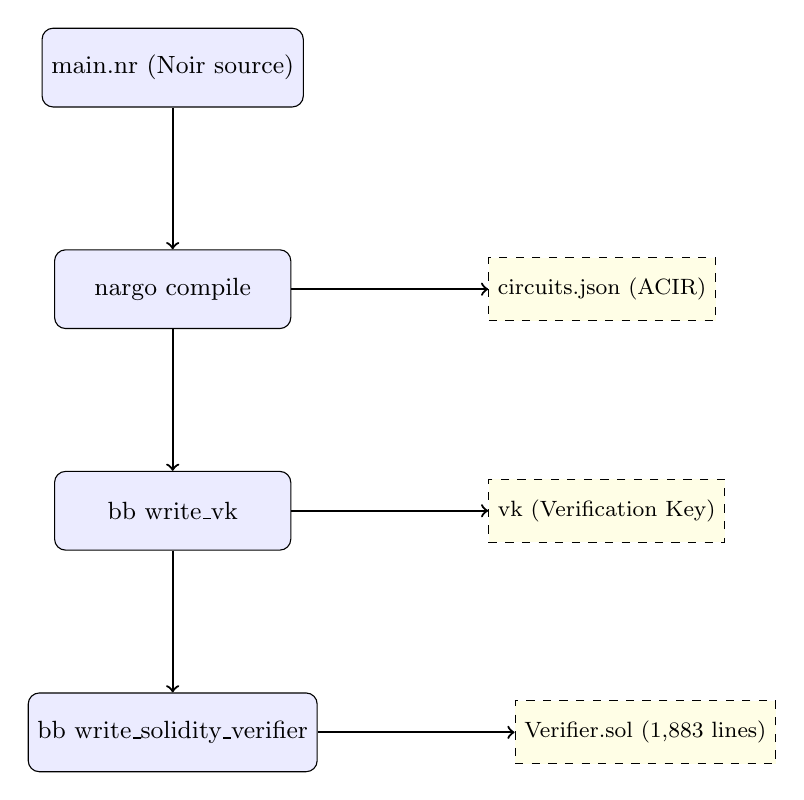
\begin{tikzpicture}[
    node distance=1.8cm,
    box/.style={rectangle, draw, rounded corners, minimum width=3cm, minimum height=1cm, text centered, font=\small, fill=blue!8},
    arrow/.style={->, thick},
    output/.style={rectangle, draw, dashed, minimum width=2.5cm, minimum height=0.8cm, text centered, font=\footnotesize, fill=yellow!10}
]
    \node[box] (source) {main.nr (Noir source)};
    \node[box, below=of source] (compile) {nargo compile};
    \node[output, right=2.5cm of compile] (json) {circuits.json (ACIR)};
    \node[box, below=of compile] (writevk) {bb write\_vk};
    \node[output, right=2.5cm of writevk] (vk) {vk (Verification Key)};
    \node[box, below=of writevk] (writesol) {bb write\_solidity\_verifier};
    \node[output, right=2.5cm of writesol] (sol) {Verifier.sol (1,883 lines)};
    
    \draw[arrow] (source) -- (compile);
    \draw[arrow] (compile) -- (json);
    \draw[arrow] (compile) -- (writevk);
    \draw[arrow] (writevk) -- (vk);
    \draw[arrow] (writevk) -- (writesol);
    \draw[arrow] (writesol) -- (sol);
\end{tikzpicture}
\caption{Circuit compilation pipeline from Noir source to on-chain Solidity verifier}
\label{fig:compile_pipeline}
\end{figure}

The compilation commands (executed in WSL Ubuntu):
\begin{lstlisting}[basicstyle=\ttfamily\footnotesize, frame=single, backgroundcolor=\color{gray!5}]
# Step 1: Compile Noir circuit to ACIR bytecode
nargo compile

# Step 2: Generate verification key from bytecode
bb write_vk --oracle_hash keccak -b ./target/circuits.json -o ./target/

# Step 3: Generate Solidity verifier from verification key
bb write_solidity_verifier -k ./target/vk -o ./target/Verifier.sol
\end{lstlisting}

\textbf{Key point:} The \texttt{--oracle\_hash keccak} flag ensures compatibility with Ethereum's native hash function, making the generated verifier directly deployable to any EVM chain.

\newpage
\subsection{Smart Contract Architecture}

\begin{figure}[H]
\centering
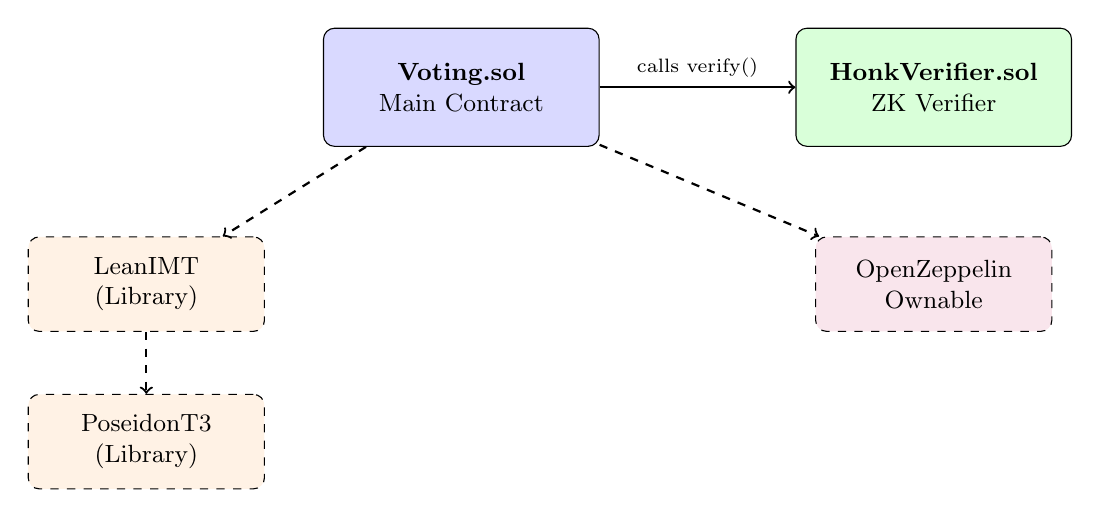
\begin{tikzpicture}[
    box/.style={rectangle, draw, rounded corners, minimum width=3.5cm, minimum height=1.5cm, text centered, font=\small, align=center},
    lib/.style={rectangle, draw, dashed, rounded corners, minimum width=3cm, minimum height=1.2cm, text centered, font=\small, align=center},
    arrow/.style={->, thick}
]
    \node[box, fill=blue!15] (voting) at (0,0) {\textbf{Voting.sol}\\Main Contract};
    \node[box, fill=green!15] (verifier) at (6,0) {\textbf{HonkVerifier.sol}\\ZK Verifier};
    \node[lib, fill=orange!10] (leanimt) at (-4,-2.5) {LeanIMT\\(Library)};
    \node[lib, fill=orange!10] (poseidon) at (-4,-4.5) {PoseidonT3\\(Library)};
    \node[lib, fill=purple!10] (ownable) at (6,-2.5) {OpenZeppelin\\Ownable};
    
    \draw[arrow] (voting) -- node[above]{\scriptsize calls verify()} (verifier);
    \draw[arrow, dashed] (voting) -- (leanimt);
    \draw[arrow, dashed] (leanimt) -- (poseidon);
    \draw[arrow, dashed] (voting) -- (ownable);
\end{tikzpicture}
\caption{Smart contract architecture showing dependencies between contracts and libraries}
\label{fig:contract_arch}
\end{figure}

\subsubsection{Voting.sol - Main Contract}

The main contract manages the entire voting lifecycle. Its state variables:

\begin{lstlisting}[style=solidity, caption={Voting contract core state}, label={lst:voting_state}]
contract Voting is Ownable {
    using LeanIMT for LeanIMTData;
    
    string private s_question;           // Election question
    IVerifier public immutable i_verifier; // ZK verifier address
    mapping(address => bool) private s_voters;        // Allowlist
    mapping(address => bool) private s_hasRegistered; // Registration flag
    mapping(uint256 => bool) private s_commitments;   // Used commitments
    mapping(bytes32 => bool) private s_nullifierHashes; // Spent nullifiers
    LeanIMTData private s_tree;          // Merkle tree (frontier-based)
    uint256 private s_yesVotes;          // Yes vote counter
    uint256 private s_noVotes;           // No vote counter
}
\end{lstlisting}

\subsubsection{Registration Function}

The \texttt{register()} function implements three security gates:

\begin{lstlisting}[style=solidity, caption={Registration logic with security checks}, label={lst:register}]
function register(uint256 _commitment) public {
    // Gate 1: Caller must be in voter allowlist
    if (!s_voters[msg.sender]) revert Voting__NotAVoter();
    
    // Gate 2: Caller must not have already registered
    if (s_hasRegistered[msg.sender]) revert Voting__AlreadyRegistered();
    
    // Gate 3: Commitment must be unique (prevent replay)
    if (s_commitments[_commitment]) 
        revert Voting__CommitmentAlreadyUsed(_commitment);
    
    // Insert commitment into Merkle tree
    s_tree.insert(PoseidonT3.hash([_commitment, _commitment]));
    s_hasRegistered[msg.sender] = true;
    s_commitments[_commitment] = true;
    
    emit NewLeaf(s_tree.size - 1, _commitment);
}
\end{lstlisting}

\subsubsection{Vote Function with ZK Verification}

The vote function is the most critical-it verifies the ZK proof and counts the vote:

\begin{lstlisting}[style=solidity, caption={Vote function with on-chain ZK proof verification}, label={lst:vote_function}]
function vote(
    bytes memory _proof, 
    bytes32 _nullifierHash,
    bytes32 _root, 
    bytes32 _vote, 
    bytes32 _depth
) public {
    // Validate tree is not empty
    if (_root == bytes32(0)) revert Voting__EmptyTree();
    
    // Validate root matches current on-chain tree state
    if (_root != bytes32(s_tree.root())) 
        revert Voting__InvalidRoot();
    
    // Assemble public inputs array for verifier
    bytes32[] memory publicInputs = new bytes32[](4);
    publicInputs[0] = _nullifierHash;
    publicInputs[1] = _root;
    publicInputs[2] = _vote;
    publicInputs[3] = _depth;
    
    // Verify ZK proof on-chain (most expensive operation)
    if (!i_verifier.verify(_proof, publicInputs)) 
        revert Voting__InvalidProof();
    
    // Check nullifier hasn't been used (anti-double-vote)
    if (s_nullifierHashes[_nullifierHash]) 
        revert Voting__NullifierHashAlreadyUsed(_nullifierHash);
    s_nullifierHashes[_nullifierHash] = true;
    
    // Count the vote
    if (_vote == bytes32(uint256(1))) s_yesVotes++;
    else s_noVotes++;
    
    emit VoteCast(_nullifierHash, msg.sender);
}
\end{lstlisting}

\subsubsection{Generated ZK Verifier Properties}

\begin{table}[H]
\centering
\caption{HonkVerifier.sol properties (auto-generated from circuit)}
\label{tab:verifier_properties}
\begin{tabular}{|l|l|}
\hline
\textbf{Property} & \textbf{Value} \\ \hline
Circuit size (gates) & 19,278 \\ \hline
Public inputs & 4 (nullifier\_hash, root, vote, depth) \\ \hline
Proving scheme & UltraHonk \\ \hline
Contract size & 1,883 lines of Solidity \\ \hline
Deployment gas & $\sim$4,727,047 \\ \hline
Interface & \texttt{verify(bytes proof, bytes32[] inputs) $\rightarrow$ bool} \\ \hline
\end{tabular}
\end{table}

\newpage
\subsection{Frontend: Browser-Side Proof Generation}

The entire proof generation pipeline executes in the voter's browser-no server ever sees the private inputs:

\begin{figure}[H]
\centering
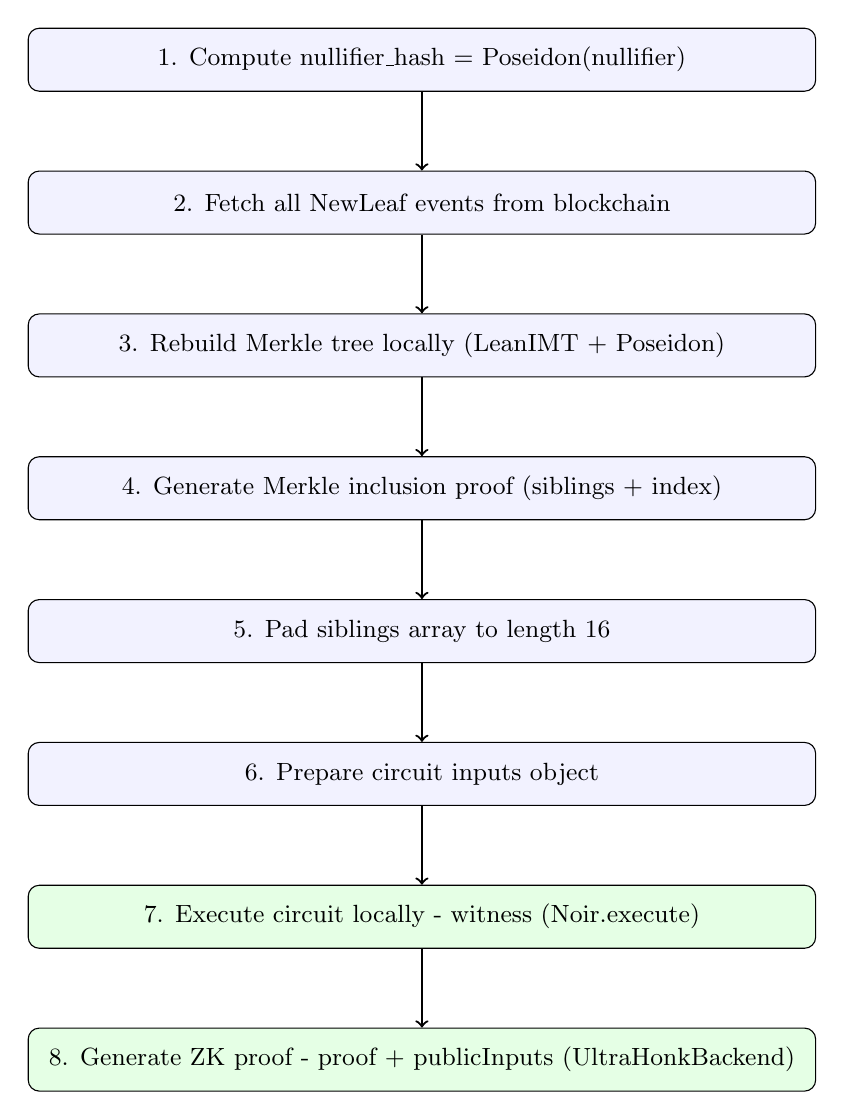
\begin{tikzpicture}[
    node distance=1cm,
    mystep/.style={rectangle, draw, rounded corners, minimum width=10cm, minimum height=0.8cm, text centered, font=\small, fill=blue!5},
    arrow/.style={->, thick}
]
    \node[mystep] (s1) {1. Compute nullifier\_hash = Poseidon(nullifier)};
    \node[mystep, below=of s1] (s2) {2. Fetch all NewLeaf events from blockchain};
    \node[mystep, below=of s2] (s3) {3. Rebuild Merkle tree locally (LeanIMT + Poseidon)};
    \node[mystep, below=of s3] (s4) {4. Generate Merkle inclusion proof (siblings + index)};
    \node[mystep, below=of s4] (s5) {5. Pad siblings array to length 16};
    \node[mystep, below=of s5] (s6) {6. Prepare circuit inputs object};
    \node[mystep, below=of s6, fill=green!10] (s7) {7. Execute circuit locally - witness (Noir.execute)};
    \node[mystep, below=of s7, fill=green!10] (s8) {8. Generate ZK proof - proof + publicInputs (UltraHonkBackend)};
    
    \draw[arrow] (s1) -- (s2);
    \draw[arrow] (s2) -- (s3);
    \draw[arrow] (s3) -- (s4);
    \draw[arrow] (s4) -- (s5);
    \draw[arrow] (s5) -- (s6);
    \draw[arrow] (s6) -- (s7);
    \draw[arrow] (s7) -- (s8);
\end{tikzpicture}
\caption{Eight-step browser-side proof generation pipeline. Steps 7--8 (green) use WebAssembly for cryptographic computation.}
\label{fig:proof_pipeline}
\end{figure}

\textbf{Why rebuild the Merkle tree in the browser?}

The smart contract stores the Merkle tree in a frontier format (only the rightmost node at each level). There is no efficient on-chain function to retrieve arbitrary Merkle proofs. Therefore, the frontend:
\begin{enumerate}
    \item Fetches all \texttt{NewLeaf} events (containing leaf values and indices)
    \item Reconstructs the complete tree using the same Poseidon hash function
    \item Generates the inclusion proof locally
\end{enumerate}

The \texttt{@zk-kit/lean-imt} TypeScript library produces identical tree structures to its Solidity counterpart, ensuring the locally-computed root always matches the on-chain root.

\newpage
\subsection{Anonymous Vote Submission}

\subsubsection{The Linkability Problem}

If the voter submits the proof from the same blockchain address they registered with, an on-chain observer could trivially link the registration transaction to the vote transaction-breaking anonymity despite the ZK proof.

\subsubsection{Solution: Identity Separation via Burner Wallets}

\begin{enumerate}
    \item \textbf{Generate fresh wallet:} \texttt{generatePrivateKey()} creates a cryptographically random Ethereum private key (no prior transaction history)
    \item \textbf{Fund the wallet:} On local Hardhat, \texttt{setBalance} provides gas. On production, a relay/paymaster would be used.
    \item \textbf{Submit vote:} The fresh wallet calls \texttt{Voting.vote(proof, publicInputs)}
    \item \textbf{Discard:} The wallet is no longer needed after voting
\end{enumerate}

On the custom blockchain (Track B), this problem is eliminated entirely-there are no wallets or gas fees; the ZK proof itself serves as authentication.

\subsubsection{Privacy Analysis}

\begin{table}[H]
\centering
\caption{Information visible vs.\ hidden to on-chain observers}
\label{tab:privacy_analysis}
\begin{tabular}{|p{6cm}|p{6cm}|}
\hline
\textbf{Visible On-Chain} & \textbf{Hidden (Private)} \\ \hline
Anonymous address called \texttt{vote()} & Who controls that address \\ \hline
Vote choice (Yes/No) & Which registered voter cast it \\ \hline
Nullifier hash (unique per voter) & The nullifier preimage \\ \hline
ZK proof blob ($\sim$14KB) & The voter's leaf index \\ \hline
Merkle root + tree depth & The sibling path \\ \hline
Timestamp of vote TX & When the voter registered \\ \hline
\end{tabular}
\end{table}

\subsection{Complete Data Flow}

\begin{figure}[H]
    \centering
    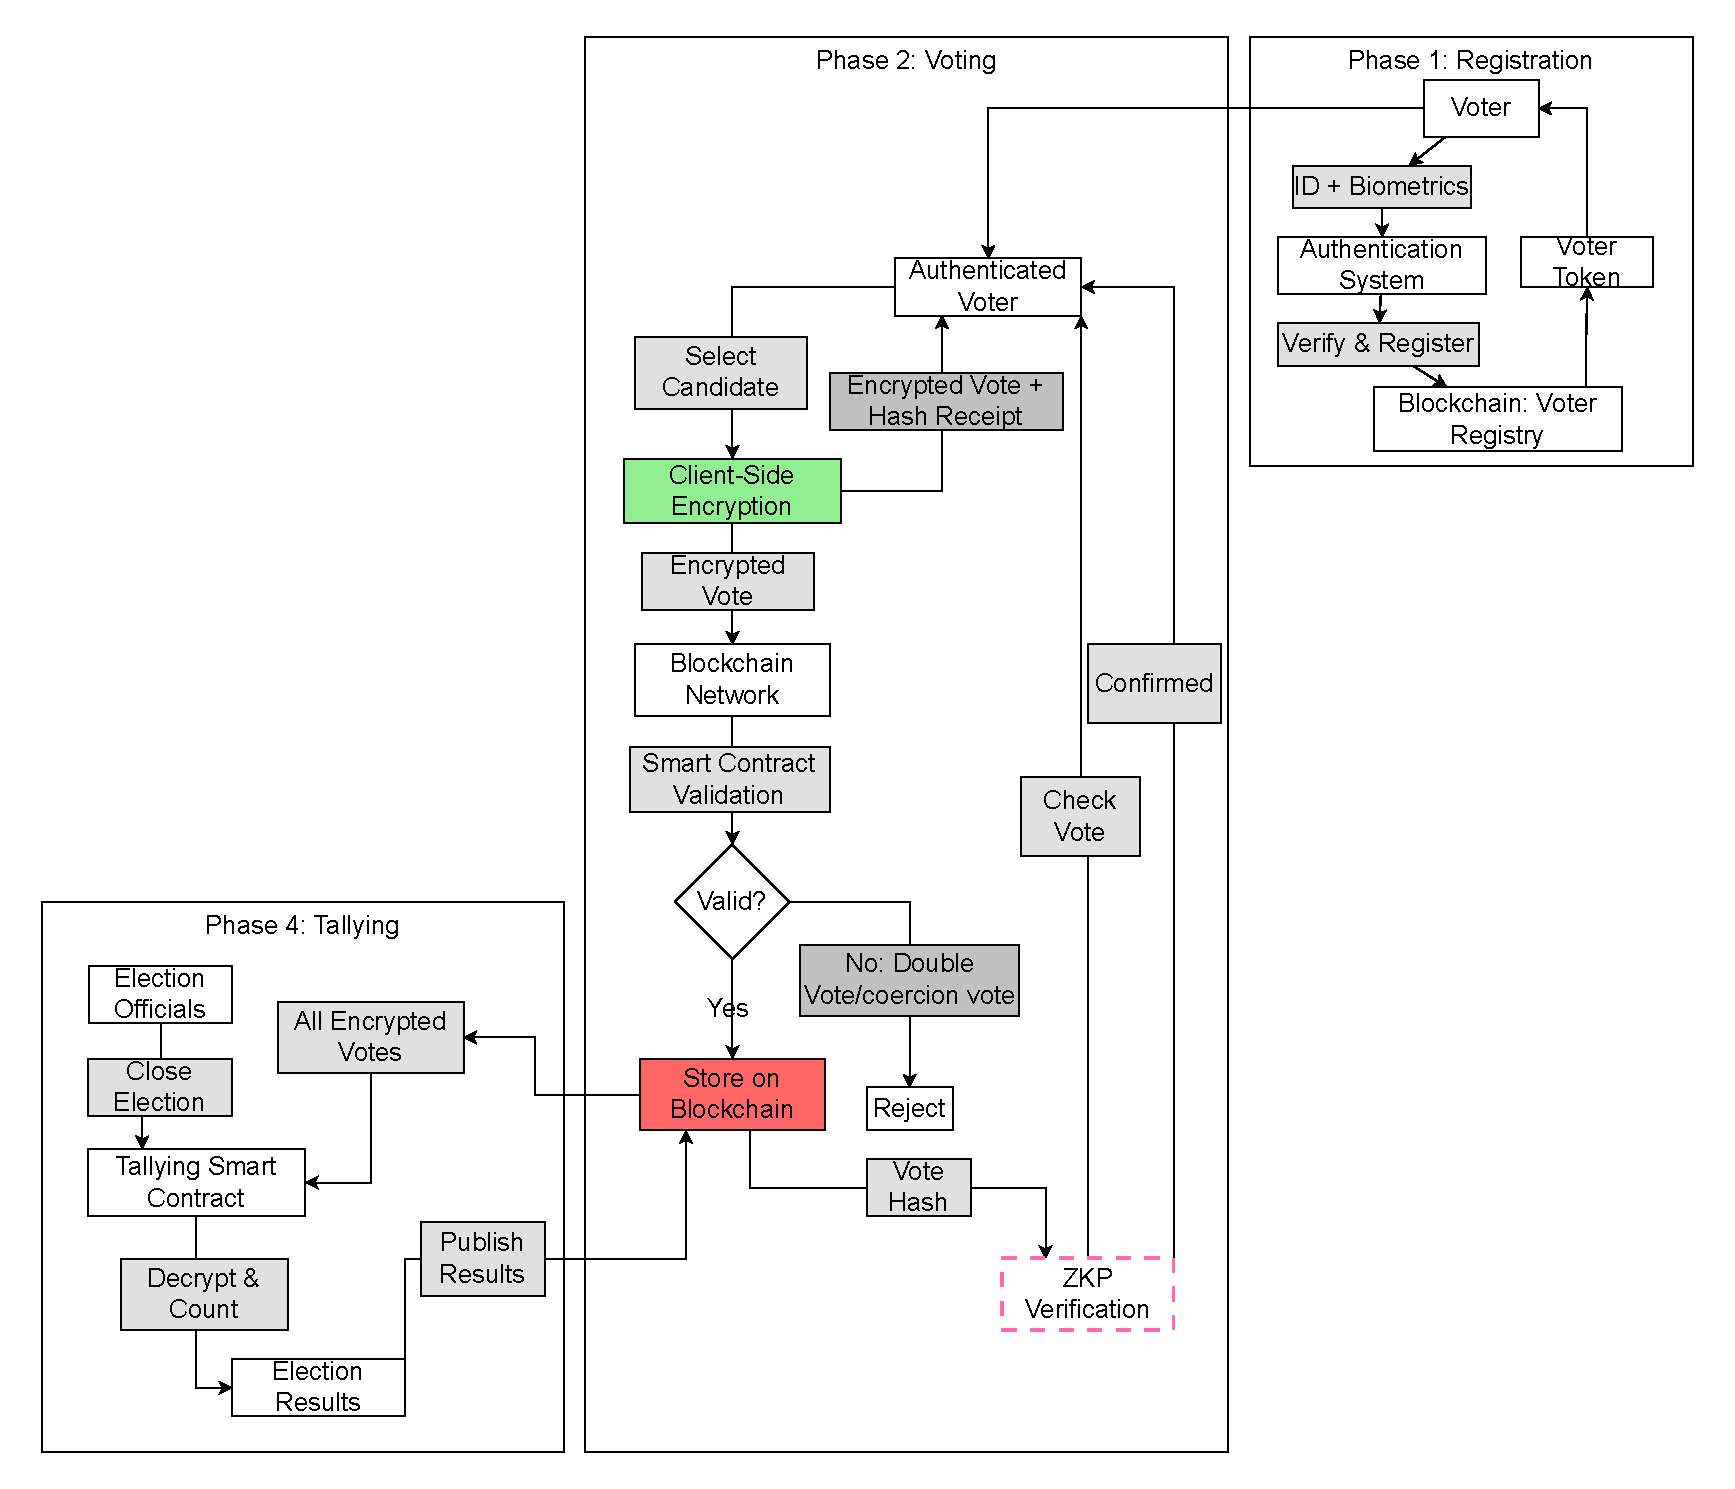
\includegraphics[width=\textwidth]{data flow.pdf}
    \caption{Complete data flow from voter registration through anonymous vote casting}
    \label{fig:data_flow}
\end{figure}

\subsection{Frontend Component Architecture}

\begin{table}[H]
\centering
\caption{Frontend component responsibilities}
\label{tab:components}
\begin{tabular}{|l|p{8cm}|}
\hline
\textbf{Component} & \textbf{Responsibility} \\ \hline
\texttt{VotingStats.tsx} & Reads on-chain state and displays live vote statistics \\ \hline
\texttt{CreateCommitment.tsx} & Generates nullifier + secret, computes commitment, registers on-chain \\ \hline
\texttt{VoteChoice.tsx} & Yes/No vote selector; stores choice in Zustand \\ \hline
\texttt{GenerateProof.tsx} & Fetches circuit, rebuilds tree, generates ZK proof \\ \hline
\texttt{VoteWithBurnerHardhat.tsx} & Creates burner wallet, funds it, submits proof \\ \hline
\texttt{AddVotersModal.tsx} & Owner-only batch voter allowlisting \\ \hline
\end{tabular}
\end{table}

\subsection{State Management and Persistence}

Cross-component state is managed by a Zustand store:

\begin{lstlisting}[style=typescript, caption={Zustand state store structure}, label={lst:store}]
type VotingState = {
  commitmentData: { 
    commitment: string; nullifier: string; 
    secret: string; index: number 
  } | null;
  proofData: { proof: Uint8Array; publicInputs: string[] } | null;
  voteChoice: boolean | null;
};
\end{lstlisting}

Commitment data, proof data, and wallet details are also persisted in localStorage (keyed by contract address and user address) to survive page reloads.

\subsection{Gas Cost Analysis}

\begin{table}[H]
\centering
\caption{Gas costs for key operations on Ethereum-compatible chain}
\label{tab:gas_costs}
\begin{tabular}{|l|r|l|}
\hline
\textbf{Operation} & \textbf{Gas Used} & \textbf{Notes} \\ \hline
Deploy PoseidonT3 & $\sim$3,700,000 & One-time library \\ \hline
Deploy LeanIMT & $\sim$1,000,000 & One-time library \\ \hline
Deploy HonkVerifier & $\sim$4,727,047 & One-time verifier \\ \hline
Deploy Voting & $\sim$672,000 & One-time contract \\ \hline
\texttt{addVoters()} (1 voter) & $\sim$72,412 & Admin operation \\ \hline
\texttt{register()} (first leaf) & $\sim$142,660 & Merkle tree insert \\ \hline
\texttt{register()} (second leaf) & $\sim$181,833 & Grows slightly \\ \hline
\texttt{vote()} with ZK verification & $\sim$300K--500K & Proof verification \\ \hline
\end{tabular}
\end{table}

\textbf{Note:} These gas costs are one of the primary motivations for Track B (custom blockchain), which eliminates gas entirely.

\subsection{Testing Methodology}

The smart contracts are tested using Hardhat's testing framework with Chai assertions:

\begin{table}[H]
\centering
\caption{Test coverage summary}
\label{tab:tests}
\begin{tabular}{|l|c|p{5.5cm}|}
\hline
\textbf{Category} & \textbf{Tests} & \textbf{What Is Verified} \\ \hline
Registration (success) & 5 & Commitment insertion, events, tree updates \\ \hline
Registration (reverts) & 3 & Non-allowlisted, double reg, duplicate commitment \\ \hline
Voter management & 2 & Batch add, view functions \\ \hline
View functions & 1 & getVotingData returns correct structure \\ \hline
\textbf{Total} & \textbf{11} & \textbf{All passing (741ms)} \\ \hline
\end{tabular}
\end{table}

\newpage
\section{Track B: Custom Purpose-Built Blockchain}

\subsection{Motivation for a Purpose-Built Blockchain}

The first Zero-Knowledge (ZK) voting app (Track A) is able to create privacy-preserving elections on an Ethereum-compatible infrastructure, but with a lot of friction involved when it comes to specific use cases. For this reason, general purpose chains such as Ethereum offer the ability to run arbitrary Turing complete smart contracts in an open environment, where no party has permission \cite{buterin2014ethereum}.

Formal elections, however, are processes which are structured, constrained, and authority administered. The native requirement of any cryptocurrency to prevent spam of network, the complex client-side wallet management (e.g., MetaMask) and the computational cost of the Ethereum Virtual Machine (EVM) are some of the dependencies that rely on Ethereum introduces. The system will remove these architectural redundancies by moving to the custom designed blockchain. Completely independent of any cryptocurrency, the custom chain also requires no browser extensions or burner wallets and relies exclusively on the ZK proof as the only authentication process, which ensures a seamless voter experience. Table \ref{tab:eth_overhead} shows the unnecessary complication comes with the general purpose blockchains that will eleminated with a custom blockchain.

\begin{table}[H]
\centering
\caption{Ethereum generalized features vs.\ specific election requirements}
\label{tab:eth_overhead}
\begin{tabular}{|l|c|p{8cm}|}
\hline
\textbf{Ethereum Feature} & \textbf{Required?} & \textbf{Architectural Rationale} \\ \hline
Mining / Proof of Stake & No & Elections are administered by a trusted authority; decentralized consensus is unnecessary. \\ \hline
Gas fees / ETH currency & No & Voters must not be burdened with acquiring cryptocurrency to participate. \\ \hline
MetaMask / Web3 Wallets & No & Adds significant UX friction and requires third-party browser extensions. \\ \hline
EVM execution engine & No & Election state transitions are highly deterministic; a Turing-complete VM is architectural overkill. \\ \hline
Burner wallets & No & The custom API is inherently identity-free; the ZK proof serves as the authorization token. \\ \hline
\end{tabular}
\end{table}

\subsection{System Architecture}

The custom blockchain is designed as a lightweight, modular application which is developed in Go. The architecture separates the verification of the cryptographic elements from the management of the state, and from the persistence of the ledger, which makes it easy to be high-performing, testable, and maintainable.

\begin{table}[H]
\centering
\caption{Custom blockchain modular architecture}
\label{tab:blockchain_modules}
\begin{tabular}{|l|l|p{7cm}|}
\hline
\textbf{Module} & \textbf{Internal Path} & \textbf{Core Responsibilities} \\ \hline
Core Engine & \texttt{internal/core/} & Defines transaction structures, SHA-256 block hashing, chain validation, and genesis block instantiation. \\ \hline
Persistence & \texttt{internal/persistence/} & Handles local JSON file-based storage, ensuring the ledger can be saved and loaded deterministically. \\ \hline
State Machine & \texttt{internal/state/} & Manages the voting state logic (mirroring the original \texttt{Voting.sol} contract) and reconstructs state from chain replay. \\ \hline
Cryptography & \texttt{internal/crypto/} & Implements the Lean Incremental Merkle Tree (LeanIMT) and Go-based Poseidon hashing over the BN254 curve. \\ \hline
REST API & \texttt{internal/api/} & Exposes HTTP endpoints with CORS support, bridging the Next.js frontend with the blockchain node. \\ \hline
\end{tabular}
\end{table}

\subsection{Data Structures and Transaction Model}

The custom blockchain does use an extremely specialized type of ledger to maintain the integrity and simplicity of the system. The design ensures that valid election operations are added to the chain from a high-level operational point of view, as well as a low-level technical perspective.

\subsubsection*{Non-Technical Overview}
The custom blockchain concept is the same as a digital logbook, but it is not allowed to be modified after it has been created, and it is used exclusively for the election process. The system is designed to be limited, unlike other blockchains, which are used for more complex financial operations. It only supports three types of actions: authorizing an allowed voter, committing a masked identity (registration) and lastly casting a private vote. It is very secure, streamlined and light, as it refuses any operation that goes beyond the 3 boundaries.

\subsubsection*{Technical Implementation}
Technically, the blockchain is a list of blocks, each of which is linked to the one before it by a cryptographic hash. The blocks have a SHA-256 hash of the previous block (\texttt{prev\_hash}), which means that if the history of the blocks is changed, the hash of the following blocks is changed to render the whole chain of blocks invalid. 

The system only allows a state transition for one of the following three kinds of transactions:
\begin{itemize}
    \item \textbf{\texttt{ADD\_VOTER}}: Executed exclusively by the administrative authority to populate the system's cryptographic allowlist.
    \item \textbf{\texttt{REGISTER}}: Submits a voter's anonymous commitment (a Poseidon hash of their secret and nullifier) to be inserted into the Incremental Merkle Tree.
    \item \textbf{\texttt{VOTE}}: Casts the final boolean vote alongside the generated ZK proof and nullifier, ensuring absolute privacy while cryptographically preventing double-voting.
\end{itemize}

To illustrate the underlying data structure, Listing \ref{lst:block_json} demonstrates the JSON representation of a block as it is persisted on disk. This specific block encapsulates a single \texttt{VOTE} transaction.

\begin{lstlisting}[style=golang, caption={Custom blockchain transaction types}, label={lst:block_json}]
{
  "index": 7,
  "timestamp": 1777442324969,
  "transactions": [
    {
      "id": "0254193b51ec082e",
      "type": "VOTE",
      "timestamp": 1777442324969,
      "payload": {
        "proof": "0xproof_aaa111",
        "nullifier_hash": "0xnull_hash_1",
        "root": "0xmerkle_root",
        "vote": true,
        "depth": 16
      },
      "hash": "0254193b51ec082e3656ecc9751e418945ecf4bde5fdce34714b5b8b973540d9"
    }
  ],
  "prev_hash": "6fda0d10f116aeb00287b24a07f832abe395d83774b31189e12f2585d3d3b6
  63",
  "hash": "faa79d7550f41b1620291898668f7fe44a8d698799bc97b33cfac435765d6
  96d"
}
\end{lstlisting}

The data on the blockchain does not include any personally identifiable data as can be seen in this \texttt{payload} of the \texttt{VOTE} transaction. Rather than that it uses only cryptographic artifacts: the \texttt{proof} which proves the voter's mathematical eligibility, the \texttt{nullifier\_hash} which is a serial number to ensure that no duplicate votes will be cast, the \texttt{root} which states the state of the Merkle tree when the \texttt{vote} was created, and the actual \texttt{vote} payload.

\subsection{Cryptographic Interoperability}

An important aspect of the design of the custom blockchain is the ability to share the cryptographic artifacts between the frontend client and the Go backend. The custom ledger natively uses the Poseidon hashing algorithm (which is implemented in \texttt{go-iden3-crypto}) and uses the same Noir circuit artifacts used in the Ethereum deployment.

\begin{itemize}
    \item \textbf{Circuit Definition (\texttt{main.nr}):} Remains completely unchanged.
    \item \textbf{Compiled Bytecode (\texttt{circuits.json}):} Served directly to the browser for client-side proof generation.
    \item \textbf{Verification Key (\texttt{vk}):} Utilized by the backend \texttt{bb verify} command-line interface to validate incoming proofs.
    \item \textbf{Hash Parameters:} The Go implementation is rigorously tested to ensure identical Poseidon hash outputs to the JavaScript/Noir environments.
\end{itemize}

The logic for generating the proof is done on the client browser. The change from Ethereum RPC to the custom REST API is completely hidden from the voter, offers the same guarantees of security on the client side and significantly reduces the complexity of the backend.

\subsection{Security and Privacy Guarantees}

The custom blockchain is based on an append-only ledger and zero knowledge cryptography which allows for end-to-end verifiability (E2EV) without a decentralized consensus such as Proof of Work. The system's main layer of authentication is the cryptographic proofs. The API does not need any identifier to send a vote, so there is no network-layer identity.

During the election period, the election authority maintains the persistence of the ledger, keeping the data available and in a way that resists censorship. In practice, however, the authority is still mathematically unable to create ZK proofs, decrypt a single vote or deanonymize Merkle tree commitments. This is a good way to meet the essential features of an electronic vote which is both secure and anonymous.

\subsection{Comparative Advantages Over Ethereum Deployment}

Following Table \ref{tab:custom_advantages} showcase the advantages gained by implementing a custom blockchain instead of ethereum blockchain.

\begin{table}[H]
\centering
\caption{Custom blockchain advantages for the election use case}
\label{tab:custom_advantages}
\begin{tabular}{|l|p{5cm}|p{6.5cm}|}
\hline
\textbf{Aspect} & \textbf{Ethereum Deployment} & \textbf{Custom Blockchain} \\ \hline
\textbf{Voter Cost} & Requires Gas fees per transaction & Completely free (cryptocurrency eliminated) \\ \hline
\textbf{Voter Setup} & Requires MetaMask and ETH funding & Zero setup (standard web browser only) \\ \hline
\textbf{Admin Control} & Smart contract ownership \& proxy patterns & Direct authority-based control over the ledger \\ \hline
\textbf{Throughput} & Constrained by global network ($\sim$15 TPS) & High throughput; limited only by proof verification latency ($\sim$200-500ms per proof) \\ \hline
\textbf{Storage Costs} & Exorbitantly expensive (per storage slot) & Negligible (local JSON files or traditional databases) \\ \hline
\textbf{Anonymity} & Necessitated complex ``burner wallet'' generation & The ZK proof acts directly as the network authentication \\ \hline
\end{tabular}
\end{table}


%%%%%%%%%%%%%%%%%%%%%%%%%%%%%%%%%%%%%
% CHAPTER 4: RESULTS
%%%%%%%%%%%%%%%%%%%%%%%%%%%%%%%%%%%%%
\chapter{Results}

\section{Functional Demonstration}

The Zero-Knowledge (ZK) electronic voting application, part of Track A, was successfully demonstrated, with a full end-to-end operational cycle. The deployment of the contract, client identity commitment, local proof generation and on-chain vote verification were part of the validation process.

\subsection{Contract Deployment}

All smart contracts were deployed to a local Hardhat execution environment to set up the decentralized backend infrastructure. The deployment process separates the cryptographic primitives, storage structures and verification logic into separate operational modules.

\begin{table}[H]
\centering
\caption{Contract deployment results}
\label{tab:deployment_results}
\begin{tabular}{|l|l|r|}
\hline
\textbf{Contract} & \textbf{Address} & \textbf{Gas Used} \\ \hline
PoseidonT3 & 0x5FbDB2...  & 3,700,000 \\ \hline
LeanIMT & (linked library) & 1,000,000 \\ \hline
HonkVerifier & 0x9fE46...  & 4,727,047 \\ \hline
Voting & 0xCf7Ed3...  & 672,000 \\ \hline
\textbf{Total} & & \textbf{$\sim$10,100,000} \\ \hline
\end{tabular}
\end{table}

\subsubsection*{Deployment Analysis}
Running the system architecture takes a total of about 10.1 million gas. This distribution is the result of the inherent computational complexity of zero-knowledge operations on the Ethereum Virtual Machine (EVM):
\begin{itemize}
    \item \textbf{\texttt{PoseidonT3}:} As an advanced cryptographic hash function operating natively over the BN254 elliptic curve scalar field, implementing its internal round constants and MDS matrix multiplications requires substantial on-chain bytecode, resulting in a high deployment footprint ($\sim$3.7M gas).
    \item \textbf{\texttt{HonkVerifier}:} Automatically generated by the Barretenberg proving backend, this contract embeds complex polynomial evaluation logic and hardcoded elliptic curve points from the verification key. Consequently, it commands the largest individual bytecode size ($\sim$4.7M gas).
    \item \textbf{\texttt{Voting}:} Serving as the central orchestration contract, the core voting logic is exceptionally optimized at $\sim$672,000 gas. Decoupling the heavy cryptographic verification into external libraries ensures that the core state machine remains lightweight, modular, and highly auditable.
\end{itemize}

\subsection{ZK Pipeline Verification}

The key part of the privacy preserving logic is the successful completion of the zero-knowledge compilation and proving pipeline. The entire circuit lifecycle was performed and checked with Noir compilation framework and Barretenberg CLI.

\begin{table}[H]
\centering
\caption{ZK pipeline execution results}
\label{tab:zk_results}
\begin{tabular}{|l|l|l|}
\hline
\textbf{Step} & \textbf{Command} & \textbf{Result} \\ \hline
Compile circuit & \texttt{nargo compile} & 19,278 gates \\ \hline
Generate witness & \texttt{nargo execute} & Witness solved \\ \hline
Generate proof & \texttt{bb prove} & $\sim$14KB UltraHonk proof \\ \hline
Verify off-chain & \texttt{bb verify} & ``Proof verified successfully'' \\ \hline
Verify on-chain & \texttt{HonkVerifier.verify()} & Returns \texttt{true} \\ \hline
\end{tabular}
\end{table}

\subsubsection*{Pipeline Analysis}
The result of compiling \texttt{main.nr} is an arithmetic backend circuit size of 19,278 gates. The footprint is very efficient for an application that runs in parallel 2 Poseidon hashes and dynamic Merkle tree path validation up to 16 levels deep

If the voter's private inputs (secret, nullifier, leaf index) satisfy all the mathematical constraints without arithmetic contradiction then the witness is solved and the voter has successfully solved the problem. The native backend proving engine proof payload is ~14KB, which is an UltraHonk proof payload. This proof provides a full mathematical guarantee of voter eligibility, and is successfully verified by local terminal tools and on-chain Solidity verifier.

\subsection{Security Verification}

Testing scripts were used to simulate several attack scenarios against the deployed \texttt{Voting.sol} contract, with a focus on the application's key security commitments. 

\begin{table}[H]
\centering
\caption{Security property verification results}
\label{tab:security_results}
\begin{tabular}{|l|l|l|}
\hline
\textbf{Attack Scenario} & \textbf{Expected Behavior} & \textbf{Result} \\ \hline
First valid vote & Accept, count vote & Pass \\ \hline
Same nullifier (double vote) & Revert: NullifierHashAlreadyUsed & Pass \\ \hline
Invalid ZK proof & Revert: InvalidProof & Pass \\ \hline
Wrong Merkle root & Revert: InvalidRoot & Pass \\ \hline
Non-registered voter & Cannot generate valid proof & Pass \\ \hline
Tampered vote value & Proof verification fails & Pass \\ \hline
\end{tabular}
\end{table}

\subsubsection*{Security Enforcement Rationale}
These security features are guaranteed by the underlying architecture, not by the software-level access control:
\begin{itemize}
    \item \textbf{Sybil Resistance \& Double Voting:} Because a voter's \texttt{nullifier\_hash} is deterministically derived from their secret key, submitting a second proof utilizing the same base identity inevitably generates an identical nullifier hash. The contract checks its internal \texttt{s\_nullifierHashes} mapping, instantly rejecting duplicate submissions to protect election integrity.
    \item \textbf{State Integrity (Wrong Merkle Root):} An attacker cannot validate a proof against an arbitrary, outdated, or simulated voter allowlist. The contract dynamically asserts that the public input root matches the current active state of the on-chain LeanIMT tree (\texttt{s\_tree.root()}).
    \item \textbf{Tamper-Evident Payload Binding:} Because the plaintext boolean vote choice is mathematically integrated as a public input during proof generation, any attempt by a malicious relay node to flip the vote bit in transit breaks the algebraic structure of the proof, causing on-chain verification to fail immediately.
\end{itemize}

\subsection{Automated Test Results}

The Voting.sol smart contract underwent a comprehensive testing suite of automated tests for deterministic state transitions, with dynamic runtime execution.

\begin{table}[H]
\centering
\caption{Complete automated test suite results}
\label{tab:test_results}
\begin{tabular}{|l|c|r|}
\hline
\textbf{Test Case} & \textbf{Status} & \textbf{Gas} \\ \hline
Allowlisted voter can register & Pass & 142,660 \\ \hline
Registration updates voter status & Pass & - \\ \hline
Tree root updates after registration & Pass & - \\ \hline
Multiple registrations increment depth & Pass & 181,833 \\ \hline
Sequential leaf indices emitted correctly & Pass & - \\ \hline
Non-allowlisted voter cannot register & Pass (reverts) & - \\ \hline
Double registration rejected & Pass (reverts) & - \\ \hline
Duplicate commitment rejected & Pass (reverts) & - \\ \hline
Batch voter addition works & Pass & 72,412 \\ \hline
View functions return correctly & Pass & - \\ \hline
getVotingData returns all fields & Pass & - \\ \hline
\textbf{Total: 11/11 passing} & \textbf{All Pass} & \textbf{741ms} \\ \hline
\end{tabular}
\end{table}

\subsubsection*{Execution and Scalability Analysis}
The execution of the automated test suite confirms absolute structural soundness, completing all 11 complex validation scenarios in 741 milliseconds within the local Hardhat environment. 

One important point is the gas spending of candidates while registering voters. The first insertion of leaf uses 142,660 gas. Subsequent registrations show a small gain of 181,833 gas as the LeanIMT structure grows in depth, because of the dynamic reallocation and hashing of internal nodes that are necessary. This empirical data proves that tree insertion algorithm works in logarithmic time $O(\log N)$ so that the operational costs would be predictable even if the number of voters increases. Moreover, the administrative operation is well optimised, and batch adding voters only uses 72,412 gas per execution block, spreading out the base EVM transaction cost.

\subsection{Performance Metrics}

End-to-end timing measurements evaluated the real-world operational viability of the electronic voting platform across both development environments and client hardware.

\begin{table}[H]
\centering
\caption{System performance measurements}
\label{tab:performance}
\begin{tabular}{|l|l|l|}
\hline
\textbf{Operation} & \textbf{Time} & \textbf{Environment} \\ \hline
Circuit compilation & $\sim$3 seconds & WSL Ubuntu \\ \hline
Verification key generation & $\sim$2 seconds & WSL Ubuntu \\ \hline
Browser proof generation & 5--8 seconds & Chrome/Firefox, desktop \\ \hline
On-chain vote verification & $<$1 second & Hardhat local node \\ \hline
Frontend page load & $<$2 seconds & Next.js dev server \\ \hline
Full voting cycle (user view) & $\sim$30 seconds & Including wallet interactions \\ \hline
\end{tabular}
\end{table}

\subsubsection*{Performance Evaluation}
The timing measures shows a very even workload distribution, over the client and the infrastructure in the back. Generating proof natively, directly in standard web browsers, using WebAssembly, takes only 5-8 seconds. This 10-second margin, with all the math involved in calculating multiple scalar multiplications and polynomial commitments, is pretty good User Experience (UX) for any high-security application.

On the other hand, on-chain verification takes less than a second. This verification is almost instantaneous, ensuring that backend nodes do not suffer from computational bottlenecks when verifying incoming ZK proofs, therefor it support a high number of transactions throughput during concurrent voting window.

\subsection{Proof Size Analysis}

Choosing the right zero-knowledge proving backend requires balancing between the size of the proof, the time it takes to verify and the level of security assumptions required to set it up.

\begin{figure}[H]
\centering
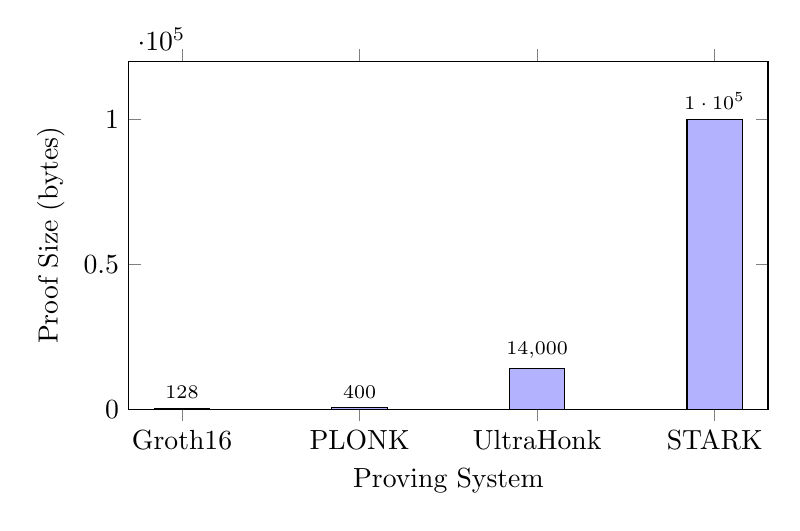
\begin{tikzpicture}
\begin{axis}[
    ybar,
    bar width=20pt,
    xlabel={Proving System},
    ylabel={Proof Size (bytes)},
    symbolic x coords={Groth16, PLONK, UltraHonk, STARK},
    xtick=data,
    nodes near coords,
    ymin=0,
    ymax=120000,
    width=0.8\textwidth,
    height=6cm,
    every node near coord/.append style={font=\scriptsize}
]
\addplot[fill=blue!30] coordinates {(Groth16, 128) (PLONK, 400) (UltraHonk, 14000) (STARK, 100000)};
\end{axis}
\end{tikzpicture}
\caption{Proof size comparison across proving systems. UltraHonk (our choice) trades larger proofs for elimination of trusted setup - a worthwhile tradeoff for election integrity.}
\label{fig:proof_size}
\end{figure}

\subsubsection*{Proving System Comparative Rationale}
As illustrated in Figure \ref{fig:proof_size} comparison, legacy proof systems such as Groth16 give very small proof sizes ($\sim$128 bytes) and a very small gas overhead required to verify the proof. But the basic security of Groth16 is based on an extremely sensitive, circuit-specific Trusted Setup ceremony. If the generated ``toxic waste'' parameters are lost or attacked, the attacker would have the opportunity to submit mathematically valid proofs to secretly influence an election.

On the other hand, STARKs are completely untethered of trusted setups, but generate very large proofs payloads ($\sim$100KB), which is cost prohibitive to store and verify directly on an EVM based layer.

This project wisely uses the ``UltraHonk'' proving system and records the optimum technical intersection. The resulting proof payload size is about 14KB, which is standard client bandwidth and EVM calldata size. Most importantly, UltraHonk is based on a universal Structured Reference String (SRS), completely removing the possibility of circuit-specific backdoors. To ensure absolute trustlessness, it is exactly the kind of integrity that is vital for public electronic elections.

\subsection{Custom Blockchain Results (Track B)}

The core foundation of the development of the purpose-built Go blockchain that will replace the Ethereum backend has been achieved.

Stage 1 implementation achieved full functional verification across the following components:
\begin{itemize}
    \item \textbf{Core Data Structures:} Engineered native Go structs for \texttt{Block} and \texttt{Transaction} models utilizing deterministic SHA-256 cryptographic linkage.
    \item \textbf{Genesis State Instantiation:} Verified the deterministic generation of the unlinked genesis block embedded with the specific election proposal question.
    \item \textbf{Tamper-Evident Engine:} Validated internal validation loops that successfully detect arbitrary state mutations or broken historical hashes across block sequences.
    \item \textbf{Persistent Storage Layer:} Successfully operationalized robust JSON file serialization and deserialization, enabling seamless state survival and deterministic reloading across node restarts.
    \item \textbf{Strict Operation Boundaries:} Successfully constrained API state models to accept only \texttt{ADD\_VOTER}, \texttt{REGISTER}, and \texttt{VOTE} transaction types, guaranteeing a minimized attack surface.
\end{itemize}


\newpage
\section{User Interface Screenshots}
Figure \ref{fig:UI-voting} illustrates the primary user interface of the Next.js frontend application. The design abstracts the underlying cryptographic complexity by guiding the voter through a sequential, structured pipeline. The interface dynamically verifies the user's eligibility via their connected wallet before unlocking the \textit{Register} function, which inserts their anonymous commitment into the Merkle tree. Following registration, the user privately selects their vote and triggers the client-side ZK proof generation. Finally, the proof is submitted to the blockchain using an automated local burner wallet, guaranteeing that the voter's primary Ethereum address is entirely decoupled from the final vote transaction.

\begin{figure}[H]
    \centering
    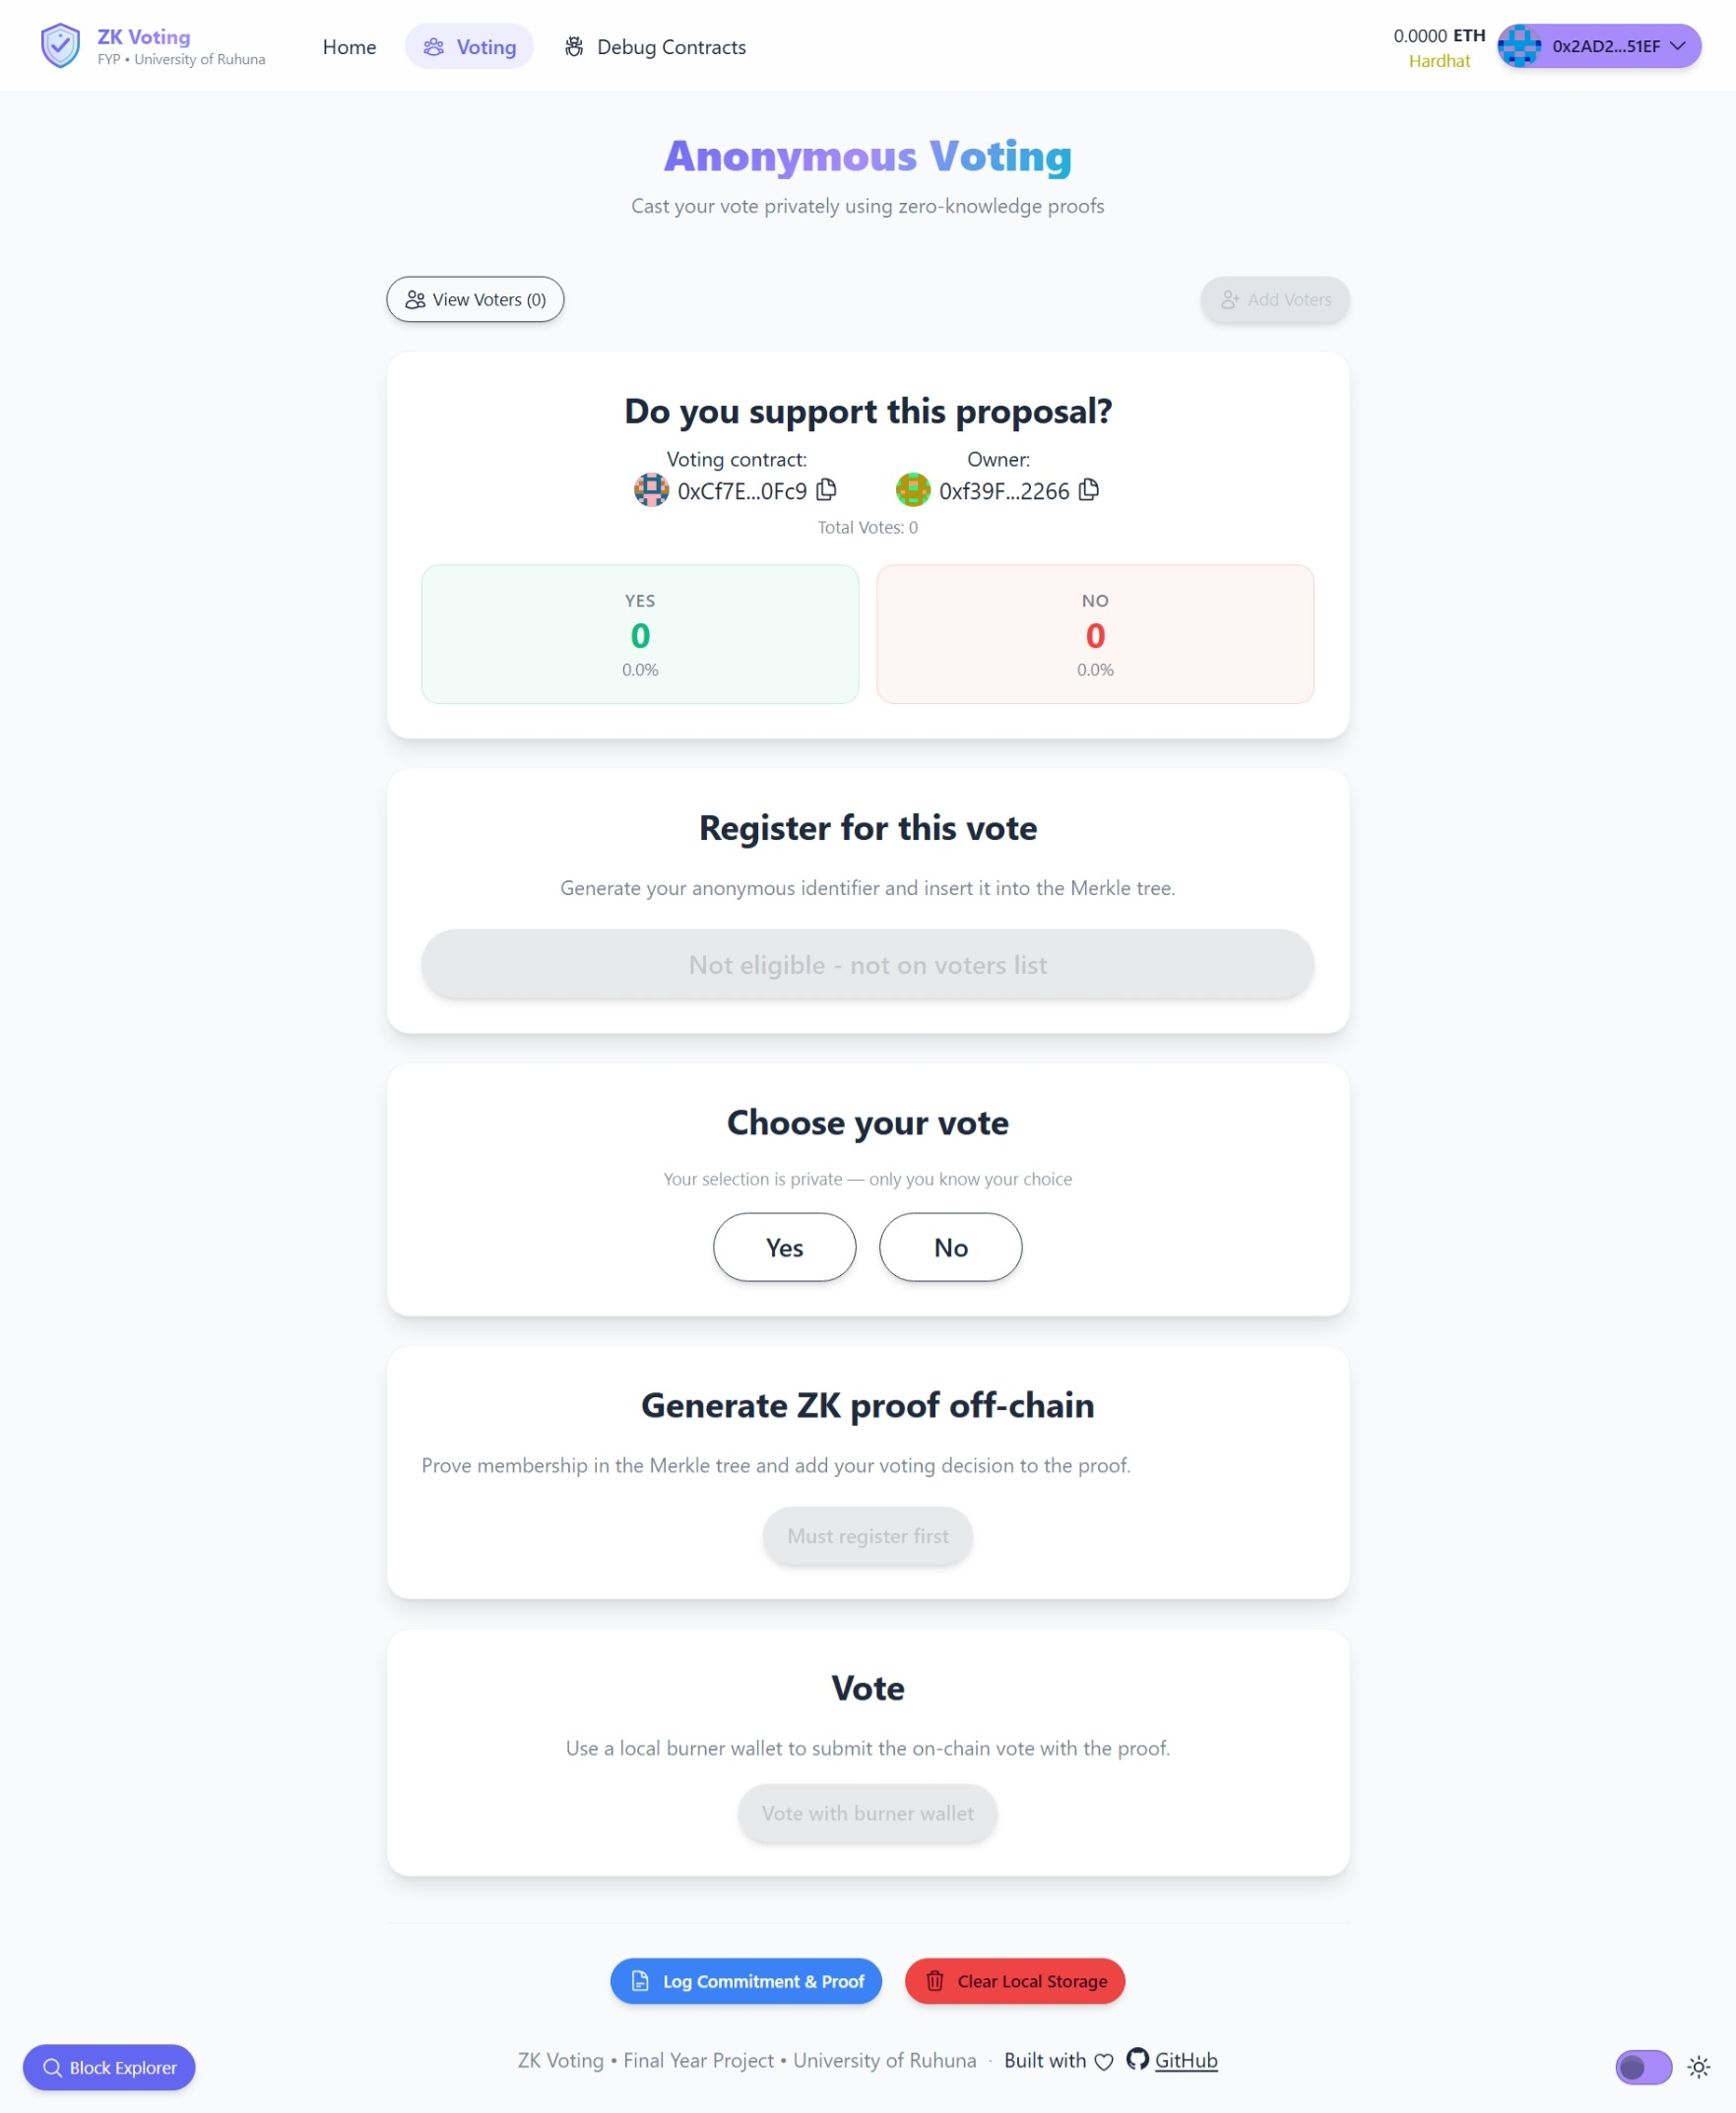
\includegraphics[width=\textwidth]{UI-voting.jpeg}
    \caption{Complete voting page interface with all workflow steps}
    \label{fig:UI-voting}
\end{figure}


\vspace{1em}
Figure \ref{fig:UI-proof generated} provides primary evidence of the client-side cryptographic execution. The browser console output confirms that the entire zero-knowledge proof generation process occurs locally within the user's browser environment via WebAssembly (WASM), ensuring that private keys and voting choices are never transmitted to a central server. The logs explicitly detail the successful generation of the witness (satisfying the Noir circuit constraints) followed by the creation of the UltraHonk proof. Notably, the output confirms the proof payload size is precisely 14,080 bytes ($\sim$14KB), validating the theoretical performance expectations of the Barretenberg backend. The final string is the ABI-encoded hex payload prepared for submission to the Solidity smart contract.

\begin{figure}[H]
    \centering
    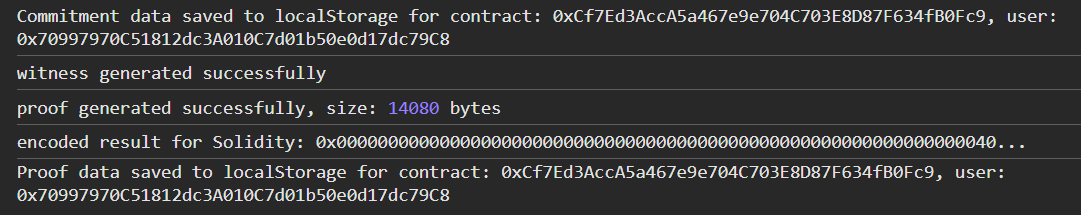
\includegraphics[width=\textwidth]{UI-proof generated.png}
    \caption{Browser console during ZK proof generation showing WASM execution}
    \label{fig:UI-proof generated}
\end{figure}


\vspace{1em}
Figure \ref{fig:vote_success} demonstrates the state of the application immediately following a successful vote submission. Once the \texttt{HonkVerifier} smart contract mathematically validates the incoming ZK proof, the blockchain state is mutated to increment the global tallies. The top panel reflects the real-time aggregate results (e.g., 2 total votes, 100\% YES) while perfectly preserving the anonymity of individual voters. The bottom panel features an integrated block explorer table that displays an immutable, auditable history of smart contract interactions. This table maps the sequential lifecycle of the election, capturing the precise block numbers and timestamps for administrative actions (\texttt{addVoters}), identity commitments (\texttt{register}), and anonymous proof submissions (\texttt{vote}).

\begin{figure}[H]
    \centering
    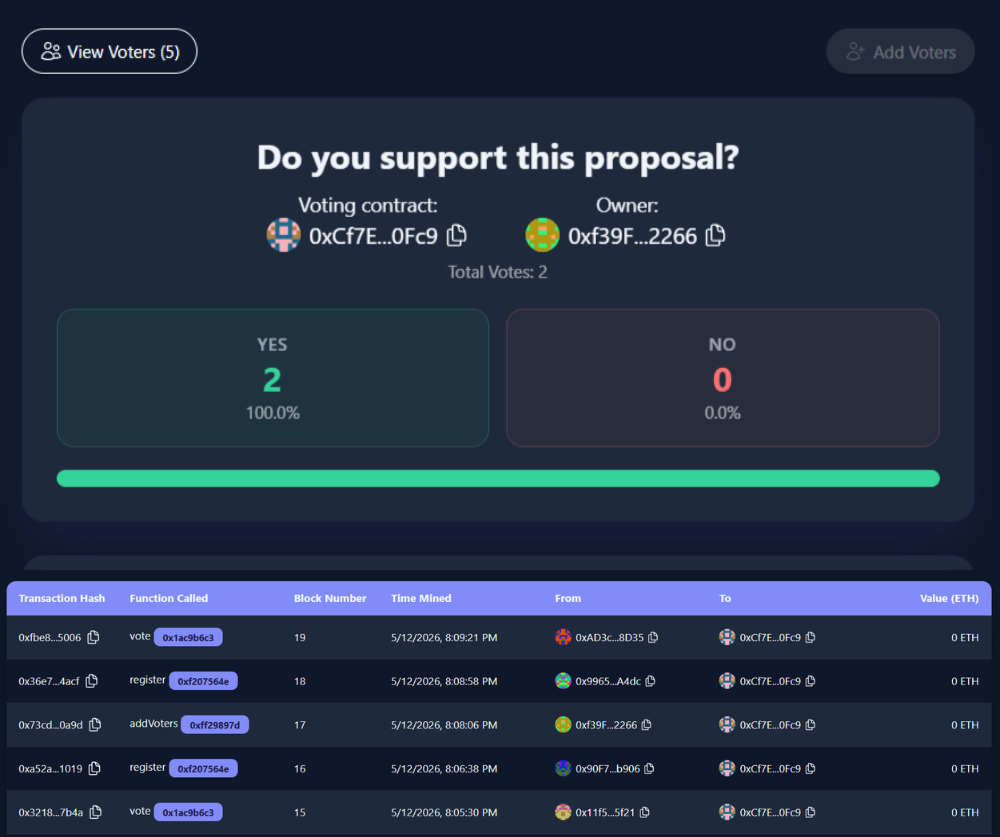
\includegraphics[width=\textwidth]{UI-Vote_Count.png}
    \caption{Successful anonymous vote submission with updated tallies}
    \label{fig:vote_success}
\end{figure}



%%%%%%%%%%%%%%%%%%%%%%%%%%%%%%%%%%%%%
% CHAPTER 5: DISCUSSION
%%%%%%%%%%%%%%%%%%%%%%%%%%%%%%%%%%%%%
\chapter{Discussion}

\section{Achievements Against Objectives}

\begin{table}[H]
\centering
\caption{Objective achievement assessment}
\label{tab:objectives_mapping}
\begin{tabular}{|c|p{4.5cm}|p{4.5cm}|c|}
\hline
\textbf{Obj.} & \textbf{Objective} & \textbf{Implementation} & \textbf{Status} \\ \hline
1 & Blockchain infrastructure & EVM contracts (functional) + Custom Go blockchain (Stage 1 complete) & Partial \\ \hline
2 & One-person-one-vote & Poseidon commitment + Merkle tree + allowlist + duplicate prevention & Achieved \\ \hline
3 & ZK proof-based privacy & UltraHonk proofs + nullifier scheme + burner wallets & Achieved \\ \hline
4 & End-to-end verifiability & On-chain proof verification + public counters + deterministic tally & Achieved \\ \hline
5 & User-friendly interfaces & Next.js web UI + 11 automated tests + full E2E demo & Achieved \\ \hline
\end{tabular}
\end{table}

\newpage
\section{Analysis of Privacy Guarantees}

Our system offers a zero-knowledge privacy instead of computational privacy, which is a critical difference with important implications for election integrity:

\begin{itemize}
	\item \textbf{Encryption-based systems} (e.g., Estonia \cite{madise2005evoting}): These systems allow the private key holder to essentially decrypt any vote. So, voter privacy is completely dependent on trust in the key holder not to look at it. From a technical point of view, if $E$ is an IND-CPA secure encryption method, privacy can be protected from outside attackers.
	
	\item \textbf{Mix-net systems} (e.g., Switzerland \cite{federalchancellery_evoting}): In this case, privacy is achieved by having a group of servers route the votes. So long as one mix server plays by the rules and remains honest, the votes remain secret. But if every $k$ servers decide to conspire secretly with one another then they can determine exactly who voted for whom.
	
	\item \textbf{Homomorphic tallying} (e.g., Helios \cite{adida2008helios}): Rather than trying to decrypt the ballots, the system mathematically totals the encrypted ballots. Here, privacy is related to a "threshold committee": a set of authorities which share portions of the main key and only allows the results of the main key to be revealed upon the joining of the members of the committee.
	
	\item \textbf{Our ZK-based system}:  It is very difficult to associate a voter with his/her ballot with our approach. The Zero-Knowledge (ZK) proof verifies the validity of a vote without revealing anything about the vote. Roughly speaking, if a distinguisher $\mathcal{D}$ is a Probabilistic Polynomial-Time (PPT) distinguisher, then its advantage in distinguishing a real proof from a simulated proof is negligible:
\end{itemize}

\begin{equation}
|\Pr[\mathcal{D}(\pi, x) = 1] - \Pr[\mathcal{D}(S(x), x) = 1]| \leq \text{negl}(\lambda)
\end{equation}

where $\pi$ is the actual proof and $S(x)$ is the generated proof (without knowledge of the witness). This is a proof with no information about the voter's identity.

\subsection{Comparison of Privacy Models}

\begin{table}[H]
\centering
\caption{Comparison of the privacy provided by various e-voting architectures}
\label{tab:privacy_models}
\begin{tabular}{|p{2.5cm}|p{2.5cm}|p{2.5cm}|p{2.5cm}|p{2.5cm}|}
\hline
\textbf{Property} & \textbf{Encryption} & \textbf{Mix-net} & \textbf{Homomorphic} & \textbf{ZK (Ours)} \\ \hline
Trust assumption & Key custodian honest & $\geq$1 mixer honest & Threshold committee & None \\ \hline
Decryption possible & Yes & Yes (if collusion) & Individual: No & No \\ \hline
Post-quantum secure & No (RSA/ECC) & Depends on cipher & No (typically) & No (BN254) \\ \hline
Voter can prove vote & Yes (receipt) & No & Depends & No (receipt-free) \\ \hline
Privacy type & Computational & Threshold & Computational & Information-theoretic* \\ \hline
\end{tabular}
\end{table}

\textit{*The property of zero-knowledge is information-theoretic in the random oracle model.}

\begin{figure}[H]
    \centering
    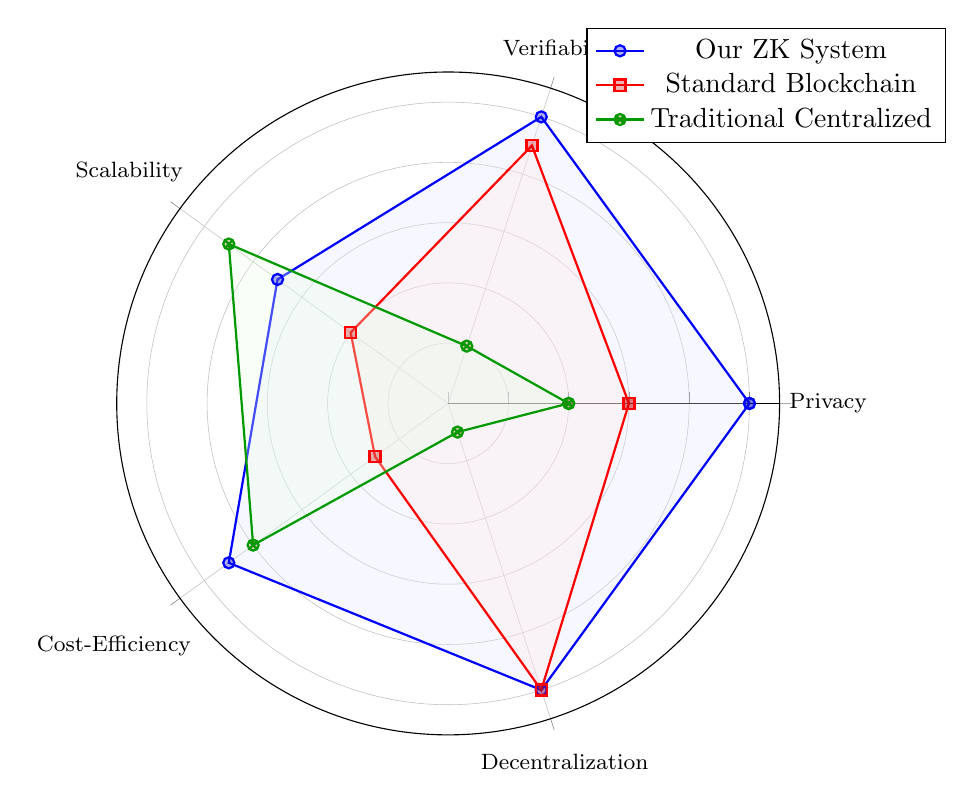
\begin{tikzpicture}
        \begin{polaraxis}[
            width=10cm,
            height=10cm,
            at={(0,0)},
            anchor=center,
            minimal/.style={mark=none, fill=none, line width=0pt},
            ticklabel style={font=\footnotesize},
            xtick={0,72,144,216,288},
            xticklabels={Privacy, Verifiability, Scalability, Cost-Efficiency, Decentralization},
            ytick={0,2,4,6,8,10},
            yticklabels={},
            limitsize/.style={min=0, max=10},
            grid=both,
            major grid style={line width=.2pt,draw=gray!50},
            minor grid style={line width=.1pt,draw=gray!20},
        ]
            % Our System (ZK-based)
            \addplot+[thick, color=blue, fill=blue!10, fill opacity=0.3] coordinates {
                (0,10) (72,10) (144,7) (216,9) (288,10) (0,10)
            };
            \addlegendentry{Our ZK System}

            % Standard Blockchain (e.g. Ethereum Voting)
            \addplot+[thick, color=red, fill=red!10, fill opacity=0.3] coordinates {
                (0,6) (72,9) (144,4) (216,3) (288,10) (0,6)
            };
            \addlegendentry{Standard Blockchain}

            % Traditional Centralized
            \addplot+[thick, color=green!60!black, fill=green!10, fill opacity=0.3] coordinates {
                (0,4) (72,2) (144,9) (216,8) (288,1) (0,4)
            };
            \addlegendentry{Traditional Centralized}
        \end{polaraxis}
    \end{tikzpicture}
    \caption{A comparative analysis of system architectures based on key performance indicators}
    \label{fig:radar_comparison}
\end{figure}

The comparative analysis in Figure~\ref{fig:radar_comparison} shows the performance of the system implemented using ZK against the traditional centralized and standard blockchain systems. In the areas of \textbf{privacy} and \textbf{verifiability} our system performs well, and the result is a resolution of the central paradox of electronic voting. The classical centralized systems have excellent \textbf{Scalability} characteristics because of their low latency database operations, but have significant shortcomings in \textbf{Decentralization} and \textbf{Verifiability}. On the other hand, traditional blockchain networks (Track A) are characterized by high decentralization but have some issues in terms of \textbf{Cost-Efficiency} (because of gas fees) and \textbf{Scalability} (due to limited scalability). In fact, the ZK-based approach on a custom blockchain (Track B) is the best of both worlds offering high integrity and privacy while also being far more cost-efficient than general purpose blockchain deployments.

\newpage
\section{Formal Correctness Analysis}

We check the correctness of our protocol with respect to the formal voting requirements laid out in Chapter 1.

\subsection{Eligibility Correctness}

\textbf{Claim:} Valid proofs can only be created by voters whose commitments are in the merkle tree.

\textbf{Argument:} Assume that an adversary $\mathcal{A}$ can construct a proof $\pi$ that would be accepted when verified for a commitment $C^*$ that is not in the tree. Then $\mathcal{A}$ has found values $(n^*, s^*, j^*, \vec{S}^*)$ such that $\text{MerkleVerify}(C^*, j^*, \vec{S}^*, d) = R$ where $R$ is the current root. However, the Merkle tree is collision resistant (Poseidon's collision resistance): If a commitment is not a member of the set, then the chance of it having a valid path to the root is limited to the collision resistance of Poseidon, $\leq 2^{-128}$.

\subsection{Uniqueness Correctness}

\textbf{Claim:} Each voter can vote only once.

\textbf{Argument:} The nullifier $n$ is set at time of registration. $N_h = \text{Poseidon}_1(n)$ is deterministic. The first vote: $N_h$ is recorded on-chain. The second time the contract tries, it checks $\texttt{s\_nullifierHashes}[N_h]$ and reverts. To vote twice $\mathcal{A}$ would have to find $n' \neq n$ such that $\text{Poseidon}_1(n') = N_h$ (second preimage) or find a commitment in the tree that is associated with a different nullifier (which would requires to register a second commitment, but this is prevented by the \texttt{s\_hasRegistered} check).

\subsection{Vote Binding Correctness}

\textbf{Claim:} The vote value can't change after proof generation.

\textbf{Argument:} The vote $v$ is a public input to the ZK circuit. The proof $\pi$ commits to the specific value of $v$ through the Fiat-Shamir transcript. If an adversary modifies $v$ to $v'$ after proof generation, the verifier recomputes the challenge using the altered public inputs, and the proof verification fails. This follows directly from the soundness property of UltraHonk: $\Pr[\text{Verify}(vk, x', \pi) = 1 \wedge x' \neq x] \leq \text{negl}(\lambda)$.

\newpage
\section{Scalability Analysis}

For any voting system to be deployed in the real world, ensuring it is scalable is crucial. We study the asymptotic complexity of each component of the system:

\begin{table}[H]
\centering
\caption{Asymptotic complexity analysis for $n$ registered voters}
\label{tab:complexity}
\begin{tabular}{|l|c|c|p{4.5cm}|}
\hline
\textbf{Operation} & \textbf{Time} & \textbf{Space} & \textbf{Notes} \\ \hline
Voter registration & $O(\log n)$ & $O(\log n)$ & Merkle tree insert (frontier update) \\ \hline
Tree reconstruction (browser) & $O(n)$ & $O(n)$ & Rebuild from events for proof generation \\ \hline
Merkle proof generation & $O(\log n)$ & $O(\log n)$ & Path extraction from local tree \\ \hline
ZK proof generation (browser) & $O(|C|)$ & $O(|C|)$ & $|C|$ = circuit size (19,278 gates), independent of $n$ \\ \hline
On-chain verification & $O(1)$ & $O(1)$ & Proof size and verifier computation are constant \\ \hline
Nullifier check & $O(1)$ & $O(n)$ & Mapping lookup; storage grows linearly \\ \hline
\end{tabular}
\end{table}

\textbf{Bottleneck analysis:} The main scalability constraint is the reconstruction of the tree in the browser, which requires downloading all $n$ \texttt{NewLeaf} events. For $n = 65{,}536$ voters, this involves $n - 1 = 65{,}535$ Poseidon hash calculations. Given an estimate of 1,500 hashes/second on WASM, this reconstruction alone takes approximately 44 seconds. When combined with the ZK proof generation time, the total process takes nearly 50 seconds, representing a significant performance bottleneck for the client-side experience.

\begin{figure}[H]
	\centering
	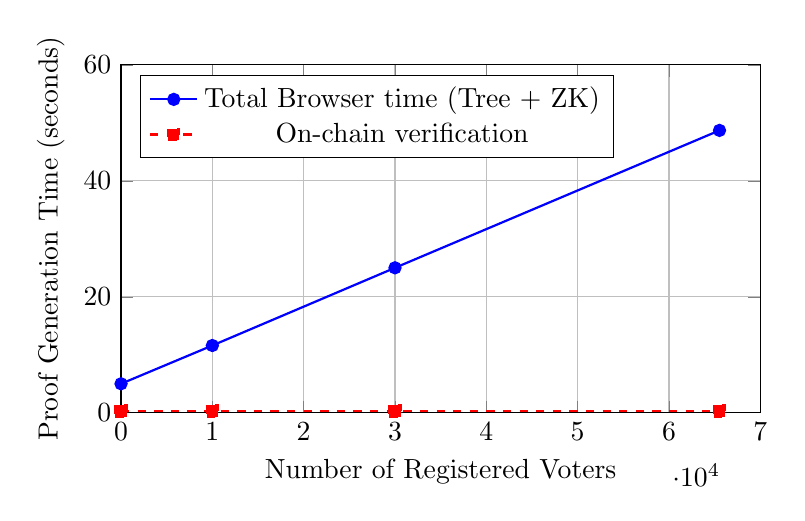
\begin{tikzpicture}
		\begin{axis}[
			xlabel={Number of Registered Voters},
			ylabel={Proof Generation Time (seconds)},
			xmin=0, xmax=70000,
			ymin=0, ymax=60,
			legend pos=north west,
			grid=major,
			width=0.8\textwidth,
			height=6cm
			]
			\addplot[color=blue, mark=*, thick] coordinates {
				(1, 5) (10000, 11.6) (30000, 25) (65536, 48.7)
			};
			\addlegendentry{Total Browser time (Tree + ZK)}
			
			\addplot[color=red, dashed, mark=square*, thick] coordinates {
				(1, 0.3) (10000, 0.3) (30000, 0.3) (65536, 0.3)
			};
			\addlegendentry{On-chain verification}
		\end{axis}
	\end{tikzpicture}
	\caption{Scalability Analysis}
	\label{fig:scalability}
\end{figure}

As shown in Figure \ref{fig:scalability}, the total client-side time scales linearly with the number of voters due to the $O(n)$ tree reconstruction cost. While the ZK proof computation and on-chain verification remain constant or logarithmic, the linear growth of the reconstruction phase becomes the dominant factor for large voter sets.


The key insight: The on-chain verification cost is constant $O(1)$ irrespective of the number of voters registered. The ZK proof is a proof that is a small enough size to contain all membership evidence. The browser side proof generation only increases marginally, $O(n)$ for the tree construction, $O(\log n)$ for the proof computation steps, whereas the proof verification and user side proof computation are unchanged.

\newpage
\section{Limitations, Challenges, and Future Work}

\subsection{Current Limitations}

\begin{enumerate}
    \item \textbf{Gas Costs (will resolve by Track B):} On-chain ZK verification gas costs 300K--500K gas per vote (will resolve by Track B). With the gas price on Ethereum mainnet around 20--50 gwei, the cost of a vote would be as high as 20--50 USD USD. The custom blockchain does not require any gas.
    
    \item \textbf{Multi-Candidate Support:} Currently, only Yes/No is supported, but in order to support multiple candidates, the circuit needs to be modified to allow for votes to be cast as integers in the range of candidates, $v \in \{0, 1, \ldots, k-1\}$, for $k$ candidates. This introduces about $\lceil \log_2 k \rceil$ extra constraints to the circuit.
    
    \item \textbf{Voter Authentication:} Manual voter addition is necessary for the allowlist-based system: Voter Authentication. Future work: Integration with decentralized identity (Worldcoin, government eID). This is a deployment challenge not a cryptographic challenge.
    
    \item \textbf{Coercion Resistance:} Receipt-free (the voter is unable to provide evidence to a third party of his/her vote), but does not support re-voting for greater coercion resistance. If re-voting was allowed, the nullifier scheme would need to be changed to allow multiple nullifier hashes per voter, but only count the last vote.
    
    \item \textbf{Root Freshness:} If there are new voters registered between the proof generation and the voting, then the root will change and the proof will be invalid. This can be solved with a root history mechanism, which requires $O(k)$ extra storage, and keeps the last $k$ valid roots.
    
    \item \textbf{Custom Blockchain Completion:}  Track B Stages 2-7 is currently being developed by the team members.
    
    \item \textbf{Post-Quantum Security:} UltraHonk is based on elliptic curve BN254 which is vulnerable to Shor's algorithm. For future quantum security, more compact proofs would need to be migrated to lattice-based or hash-based proof systems, such as STARKs.
\end{enumerate}

\subsection{Technical Challenges Encountered}

While implementing, some major technical issues were found and addressed:

\begin{enumerate}
    \item \textbf{Hash Function Compatibility:} The hash functions in Poseidon must return the same results in three different environments: Noir circuits (field arithmetic), Solidity smart contracts (uint256), and TypeScript frontend (BigInt). If there are any differences with round constants, field modulus, or endianness, proof verification fails. We addressed this by employing the \texttt{@zk-kit} library family, which offers cross-platform implementations of Poseidon that are verified.
    
    \item \textbf{WASM Memory Constraints:}  It takes about 256 MB of memory to generate proofs with the Barretenberg WASM module. This is not possible in some mobile browsers and older devices, restricting access. We detect support for WASM and memory availability before trying to generate a proof to mitigate this.
    
    \item \textbf{Circuit Compilation Toolchain:}  The Noir/Barretenberg toolchain does need WSL (Windows Subsystem for Linux) on Windows machines, which adds to the development complexity. The flag \texttt{--oracle\_hash keccak} for the generation of verifiers for Ethereum compatible chains was not mentioned in the main Noir documentation, and had to be studied from the Barretenberg source code.
    
    \item \textbf{Merkle Tree Frontier Format:} The on-chain LeanIMT only contains frontier nodes (rightmost path), not the whole tree. This design reduces gas expenses, but requires the frontend to rebuild the tree from the events logs, an architectural requirement that was identified during integration testing.
\end{enumerate}

\subsection{Future Research Directions}

\begin{enumerate}
    \item \textbf{Formal Verification:}  Using formal methods (such as model checking, theorem proving) to verify the correctness of the ZK circuit and smart contract logic. Machine checked proofs of contract invariants could be given by tools like Certora or K Framework.
    
    \item \textbf{Differential Privacy for Tallies:}  Individual votes are private, but the aggregate information is revealed in the final tally, which is an example of Differential Privacy for Tallies. Introducing differential privacy noise to intermediate tallies may give privacy to the aggregate, but at the cost of sacrificing accuracy.
    
    \item \textbf{Recursive Proofs for Scalability:} Batch verification of $k$ votes in one on-chain transaction, amortizing the verification cost over $k$ votes, using recursive proof composition (proof-of-proofs).
    
    \item \textbf{Decentralized Identity Integration:} Replace the allowlist mechanism with privacy-preserving voter registration verification (e.g., ZK credentials from government-issued documents) to achieve truly self-sovereign voter registration.
    
    \item \textbf{Cross-Chain Deployment:} Testing deployment on Layer 2 networks (Arbitrum, Optimism, zkSync) with gas fees 10–100 times cheaper than the Ethereum mainnet, as an alternative to the custom blockchain for organizations that want to use existing infrastructure.
\end{enumerate}


%%%%%%%%%%%%%%%%%%%%%%%%%%%%%%%%%%%%%
% CHAPTER 6: TIMELINE
%%%%%%%%%%%%%%%%%%%%%%%%%%%%%%%%%%%%%
\chapter{Timeline and Resources}

\section{Project Timeline}

The project is conducted across two academic semesters (32 weeks).

\begin{landscape}
\begin{figure}[p]
    \centering
    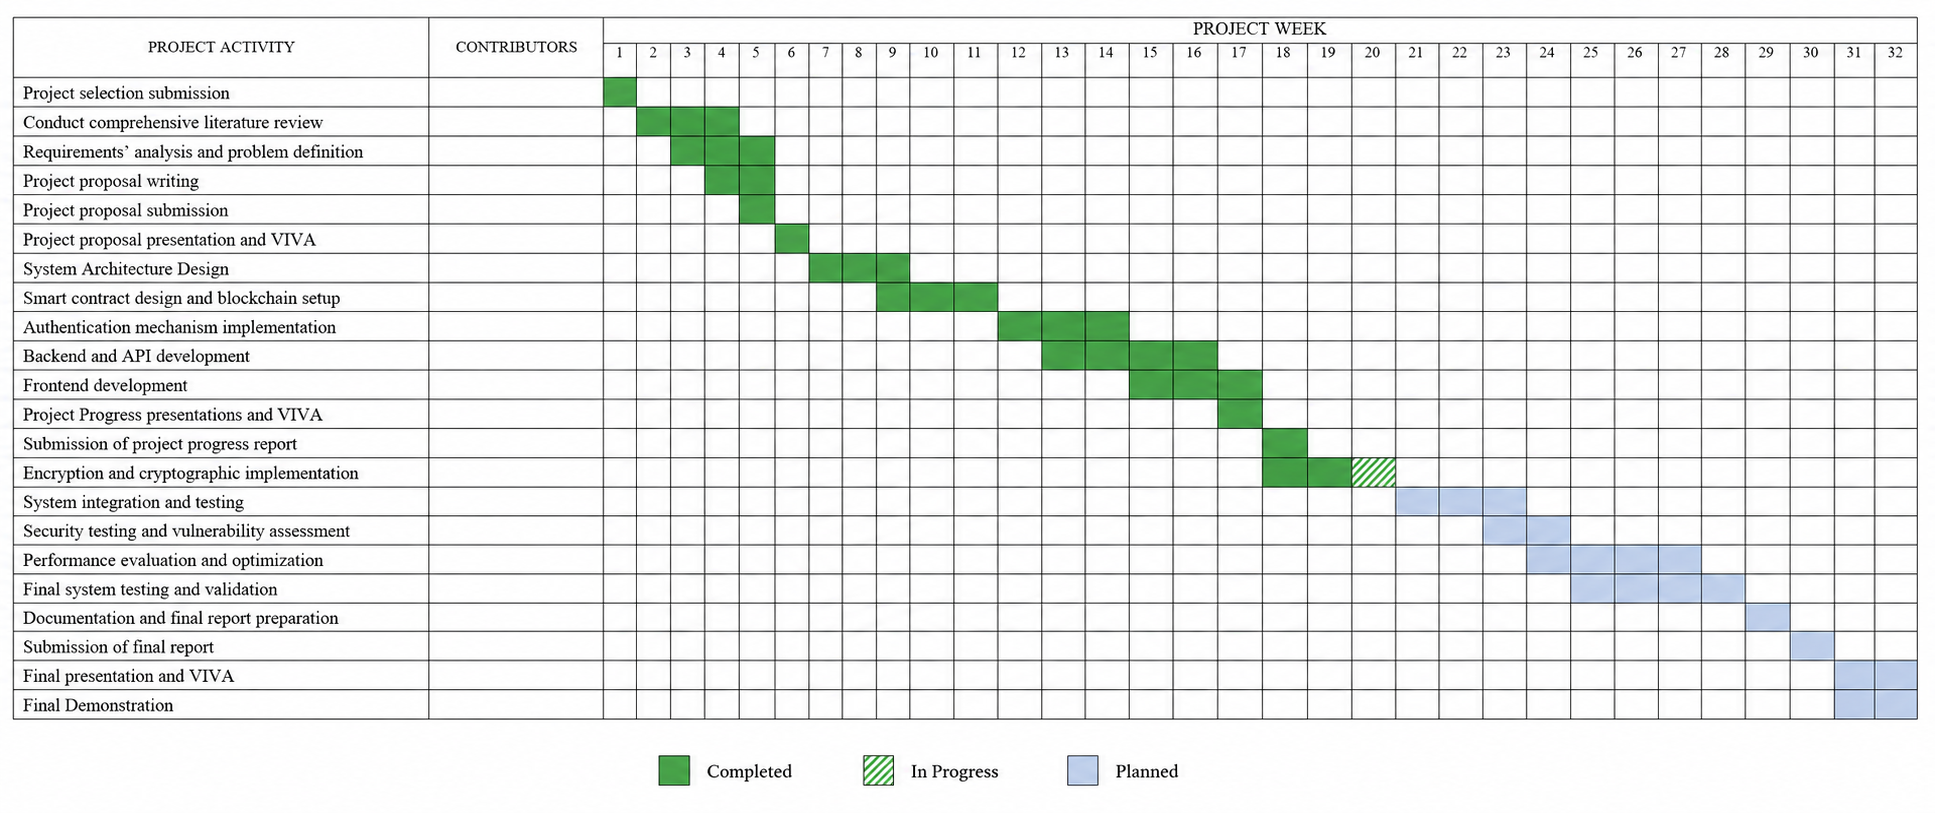
\includegraphics[width=1.7\textwidth,height=0.8\textheight]{timeline.png}
    \caption{Project timeline over two academic semesters (32 weeks)}
    \label{fig:timeline}
\end{figure}
\end{landscape}

\section{Implementation Phases}

\begin{table}[H]
\centering
\caption{Implementation phases and completion status}
\label{tab:phases}
\begin{tabular}{|c|l|c|l|}
\hline
\textbf{Phase} & \textbf{Description} & \textbf{Track} & \textbf{Status} \\ \hline
0 & Project Scaffold (Scaffold-ETH 2 + Noir) & A & Completed \\ \hline
1 & Voting Contract Structure & A & Completed \\ \hline
2 & Voter Registration with LeanIMT & A & Completed \\ \hline
3 & ZK Circuit - Commitment Scheme & A & Completed \\ \hline
4 & ZK Circuit - Merkle Root Verification & A & Completed \\ \hline
5 & Solidity Verifier Generation & A & Completed \\ \hline
6 & vote() + E2E Proof Verification & A & Completed \\ \hline
7 & Frontend UI \& Commitment Registration & A & Completed \\ \hline
8 & Browser-Side ZK Proof Generation & A & Completed \\ \hline
9 & Anonymous Vote Casting (Burner Wallet) & A & Completed \\ \hline
\hline
B1 & Blockchain Foundation (Go) & B & Completed \\ \hline
B2 & Cryptography Layer (Poseidon in Go) & B & In Progress \\ \hline
B3 & Voting State Machine & B & Planned \\ \hline
B4 & ZK Proof Verification (bb verify) & B & Planned \\ \hline
B5 & REST API Server & B & Planned \\ \hline
B6 & Integration Testing & B & Planned \\ \hline
B7 & Frontend Connection & B & Planned \\ \hline
\end{tabular}
\end{table}

\section{Resources}

\subsection{Hardware}
\begin{itemize}
    \item Personal computers (4 team members) with Windows 11 + WSL Ubuntu
    \item Minimum 8GB RAM required for browser proof generation (WASM)
\end{itemize}

\subsection{Software (All Open Source)}
\begin{itemize}
    \item Noir compiler (nargo) v1.0.0-beta.3, Barretenberg (bb) v0.82.2
    \item Go 1.22+ (custom blockchain)
    \item Node.js v20.18.3, Yarn v4.13.0
    \item Hardhat, Next.js 15, React 19, TypeScript
    \item Visual Studio Code, Git + GitHub
\end{itemize}

\subsection{Cost}
Total development cost: \textbf{\$0} - open-source tools on local infrastructure.


%%%%%%%%%%%%%%%%%%%%%%%%%%%%%%%%%%%%%
% CHAPTER 7: CONCLUSION
%%%%%%%%%%%%%%%%%%%%%%%%%%%%%%%%%%%%%
\chapter{Conclusion}

This project introduces a design, implementation and analysis of an end-to-end verifiable electronic voting system that mitigates the fundamental conflict between ballot secrecy and election integrity while preserving privacy. The system achieves the following in a novel combination of zero-knowledge proofs, on-chain verification, and cryptographic identity separation:

\begin{enumerate}
    \item \textbf{Complete voter anonymity} - no entity, not even system administrators, can know who voted for which vote by the use of zero-knowledge proofs and identity separation. This is a mathematical guarantee, not a policy guarantee. The privacy is information-theoretic in the random oracle model, that is, it cannot be broken by any computational improvement.
    
    \item \textbf{Double-vote prevention} - Each voter can cast a single vote, using deterministic nullifier hashing. If someone tries to vote again, they will find the same nullifier hash, which will be rejected. The preimage resistance of the Poseidon hash function ensures the determinism.
    
    \item \textbf{Public verifiability} - All proof verifications and vote counts are public on-chain. The election result can be independently checked by anyone by replaying the transaction history and verifying that all accepted proofs satisfy the HonkVerifier contract.
    
    \item \textbf{Client-side privacy} - proof generation is done in the voter's browser using WebAssembly. No one, including the voter, the server or the administrator, knows the voter's private inputs. This removes the need for trusted intermediaries which are characteristic of encryption-based systems \cite{madise2005evoting, federalchancellery_evoting}.
    
    \item \textbf{No trusted setup} - the UltraHonk proving system \cite{aztec2024ultrahonk} eliminates trusted setup ceremonies, which is a major attack vector in Groth16-based systems \cite{groth2016size}. The system parameters are based on publicly verifiable randomness.
    
    \item \textbf{No trusted authority for privacy} - Unlike encryption-based systems (where a key holder can decrypt) or mix-net systems (where colluding mixers can deanonymize), our ZK-based approach doesn't require any trust assumption on third parties for privacy.
\end{enumerate}

The system was developed in 10 iterative phases (Track A) and all phases were successfully completed and demonstrated. Moreover, a purpose-built blockchain (Track B) is being developed in parallel, which will remove the need for general purpose Ethereum infrastructure (including gas fees, wallet needs, EVM complexity, etc.) while maintaining all cryptographic guarantees.

\textbf{Research Contributions.} This project makes the following contributions to the field of cryptographic voting systems:
\begin{enumerate}
    \item A full and working implementation of proof generation for voting using a browser, showing that proof generation is feasible on the client side with today's hardware and WASM technology.
    \item Formal study of the security properties that can be obtained from a combination of Poseidon-based commitment schemes and UltraHonk proofs and on-chain verification.
    \item A comparative assessment with the other e-voting systems (Estonia, iVote, Swiss Post, FASTEN) and the specific privacy and trust benefits of the ZK-based approach.
    \item A dual-track design which allows for the independent development and testing of Track A (cryptographic correctness) and Track B (deployment infrastructure).
    \item Empirical metrics on proof generation time, proof size, gas cost and scalability properties that guide the real-world applicability of ZK voting.
\end{enumerate}

The project shows that modern zero-knowledge proof systems, in particular the Noir language \cite{noir2024docs} and the UltraHonk proving backend, have come of age to make practical, usable, privacy-preserving voting possible using open-source tools and standard web browsers. These formal properties of secure electronic voting (eligibility, uniqueness, privacy, verifiability) may be achieved by careful design of the cryptographic protocols without the need for trusted third parties.

Future work will involve finishing the custom blockchain integration (Stages 2--7), implementing multi-candidate support using range-checked circuit inputs, formal verification of the smart contract invariants, and exploring post-quantum alternatives to the UltraHonk's BN254 curve.

% References
\renewcommand{\bibname}{References}
\bibliographystyle{ieeetr}
\addcontentsline{toc}{chapter}{References}
\bibliography{bibliography}

\end{document}
